%%%%% Global Options

\def\showcomments{}
\def\showinlinecomments{}



\documentclass[11.5pt, a4paper]{report}

\usepackage[utf8]{inputenc}
\usepackage[english]{babel}
\usepackage[T1]{fontenc}

\usepackage{amsmath, amssymb, amscd, amsthm, amsfonts, mathtools}
\usepackage[a4paper,bindingoffset=0cm,left=2.0cm,right=2.0cm,top=2.5cm,bottom=2.5cm,footskip=1.0cm,headheight=15pt]{geometry}

\usepackage{fancyhdr}
\pagestyle{fancy}
\renewcommand{\headrulewidth}{0.8pt}
\renewcommand{\footrulewidth}{0.8pt}
\fancyhead{}
\fancyhead[C]{\leftmark}

\usepackage{graphicx}
\usepackage{xcolor}
\definecolor{darkblue}{rgb}{0.0, 0.0, 0.55}
\definecolor{darkred}{rgb}{0.55, 0.0, 0.0}
\usepackage{natbib} %%% https://www.overleaf.com/learn/latex/Bibliography_management_with_natbib
\setcitestyle{square,compress,numbers,comma}
\usepackage[final]{hyperref}
\hypersetup{
           breaklinks=true,   % splits links across lines
           colorlinks=true,   % displays links as colored text instead of blocks
           citecolor=blue,
           linkcolor=darkred,
           urlcolor=darkblue,
        }
\usepackage{physics}
\usepackage{tikz}
\usepackage{url}
\usepackage{tabularx}

\usepackage{braket}
\usepackage{thmtools}
\usepackage{float}
\usepackage{doi}
\usepackage{lipsum}
\usepackage[center]{caption}
\usepackage{subcaption}
\usepackage{listings}

% \theoremstyle{definition}
\newtheorem{theorem}{Theorem} %[section]
\newtheorem{definition}[theorem]{Definition}
\newtheorem{lemma}[theorem]{Lemma}
\newtheorem{conjecture}[theorem]{Conjecture}
\newtheorem{corollary}[theorem]{Corollary}
\newtheorem{proposition}[theorem]{Proposition}
\newtheorem*{remark}{Remark}

\numberwithin{theorem}{section}
\numberwithin{definition}{section}
\numberwithin{lemma}{section}
\numberwithin{conjecture}{section}
\numberwithin{corollary}{section}
\numberwithin{proposition}{section}
\numberwithin{equation}{section}

%% Unique hyperref anchors (avoid duplicate destinations from \numberwithin)
\renewcommand{\theHequation}{\thechapter.\thesection.\arabic{equation}}
\renewcommand{\theHtheorem}{\thechapter.\thesection.\arabic{theorem}}
\renewcommand{\theHdefinition}{\thechapter.\thesection.\arabic{definition}}
\renewcommand{\theHlemma}{\thechapter.\thesection.\arabic{lemma}}
\renewcommand{\theHconjecture}{\thechapter.\thesection.\arabic{conjecture}}
\renewcommand{\theHproposition}{\thechapter.\thesection.\arabic{proposition}}
\renewcommand{\theHcorollary}{\thechapter.\thesection.\arabic{corollary}}


\allowdisplaybreaks
\renewcommand{\thefootnote}{\roman{footnote}}

%% Autoref prefixes
\renewcommand{\sectionautorefname}{Section}
\renewcommand{\subsectionautorefname}{Section}
\renewcommand{\subsubsectionautorefname}{Section}
\def\theoremautorefname{Theorem}
\def\lemmaautorefname{Lemma}
\def\definitionautorefname{Definition}
\def\conjectureautorefname{Conjecture}
\def\corollaryautorefname{Corollary}
\def\propositionautorefname{Proposition}
\def\proofautorefname{Proof}

\definecolor{leanbg}{RGB}{246,248,250}
\definecolor{leanframe}{RGB}{214,220,230}
\definecolor{leankeyword}{RGB}{0,64,160}
\definecolor{leancomment}{RGB}{0,110,0}
\definecolor{leanstring}{RGB}{163,21,21}

\lstdefinelanguage{Lean}{
  morekeywords={
    import,namespace,end,open,variable,variables,def,abbrev,theorem,lemma,axiom,
    structure,inductive,class,instance,where,let,in,by,have,show,from,if,then,else,
    match,with,fun,forall,exists,noncomputable,deriving,set_option,attribute
  },
  sensitive=true,
  morecomment=[l]{--},
  morecomment=[s]{/-}{-/},
  morestring=[b]"
}

\lstdefinestyle{leanstyle}{
  language=Lean,
  basicstyle=\ttfamily\small,
  keywordstyle=\color{leankeyword}\bfseries,
  commentstyle=\color{leancomment},
  stringstyle=\color{leanstring},
  backgroundcolor=\color{leanbg},
  frame=single,
  rulecolor=\color{leanframe},
  framerule=0.6pt,
  xleftmargin=8pt,
  xrightmargin=8pt,
  keepspaces=true,
  columns=fullflexible,
  breaklines=true,
  showstringspaces=false,
  tabsize=2
}


% \usepackage[8-9]{pagesel} % Compile selected pages


%% Writing algorithms

\usepackage{algorithm} % captioning
\usepackage{algpseudocode}

% \def\NoNumber#1{{\def\alglinenumber##1{}\State #1}\addtocounter{ALG@line}{-1}}

\graphicspath{ {images/} }


\begin{document}

\pagenumbering{roman}

\thispagestyle{empty}
\begin{center}
\vspace*{1.5cm}
{\Large \bf Unstructured Adiabatic Quantum Optimization}

\vspace*{3.75cm}
{\large Thesis submitted in partial fulfillment\\}
{\large  of the requirements for the degree of \\}

\vspace*{1cm}
{\it {\large Master of Science in Computer Science and Engineering by Research}}

\vspace*{1cm}
{\large by}

\vspace*{5mm}
{\large Alapan Chaudhuri\\}
{\large 2019111023\\
{\small \tt alapan.chaudhuri@research.iiit.ac.in}}


\vspace*{4.0cm}
% {\psfig{figure=images/iiit.eps,width=14mm}\\}
\begin{center}
\includegraphics[width=45mm]{images/iiit-logo.png}
\end{center}
{\large Centre for Quantum Science and Technology (CQST) \\}
{\large International Institute of Information Technology (IIIT) \\}
{\large Hyderabad - 500032, India\\}
{\large February 2026\\}
\end{center}


%% COPYRIGHT PAGE
\newpage
\thispagestyle{empty}
\vspace*{\fill}
\begin{center}
    \large Public Domain\\
    Alapan Chaudhuri, 2026\\
    \large No Rights Reserved\\
\end{center}
\vspace*{\fill}


\input{frontmatter/certificate.tex}

%% DEDICATION PAGE
\newpage
\thispagestyle{empty}
\vspace*{\fill}
\begin{center}
    \large [Dedication]\\
\end{center}
\vspace*{\fill}



%% QUOTE PAGE
\newpage
\thispagestyle{empty}
\vspace*{\fill}
\begin{center}
    ``Computers are more forgiving than bare-bone nature or mathematics\\
    --- both of which are infinitely more forgiving than academia."
\end{center}
\vspace*{\fill}


\chapter*{Abstract}
\input{frontmatter/abstract.tex}

\chapter*{Acknowledgement}
\input{frontmatter/acknowledgement.tex}

\tableofcontents
\begingroup\hfuzz=3pt\listoftheorems\endgroup
\listofalgorithms
\listoffigures


\chapter{Introduction}

\pagenumbering{arabic}

% Chapter 1: Introduction (~15 pages)
% Motivation, quantum promise, central paradox, thesis contributions, roadmap



\chapter{Physics and Computation}
% Chapter 2: Physics and Computation


\chapter{Quantum Computation}
% Chapter 3 content goes here



\chapter{Adiabatic Quantum Computation}
Chapter 3 closed one model cleanly. In the circuit-query setting, unstructured
optimization is characterized by a sharp frontier,
$\Theta(\sqrt{N/d_0})$. The next question is not whether quantum mechanics helps
in principle. The next question is what happens when the same objective is
implemented by continuous Hamiltonian evolution instead of discrete oracle calls.

Adiabatic quantum computation answers that question in a physically direct way.
Prepare a ground state that is easy to initialize, deform the Hamiltonian, and
try to stay in the instantaneous ground space until the final Hamiltonian encodes
the solution. This sounds conceptually simple, and that simplicity is exactly why
it is so attractive. The technical reality is sharper. ``Slowly'' is not a vague
instruction. It is the runtime law, and the spectral gap along the interpolation
path is the central resource.

This chapter builds that framework from first principles and then narrows to the
AQO regime used in Chapters 5--8. The story has four steps. Define the model.
State the quantitative adiabatic control law. Understand avoided crossings and the
Roland-Cerf benchmark. Then confront the central tension: universality of model
power does not remove information bottlenecks in schedule design.

\section{Model}
\label{sec:ch4-aqc-model}

An adiabatic algorithm is specified by a Hamiltonian path and a monotone schedule.
The standard interpolation is
\begin{equation}
\label{eq:ch4-interpolation}
H(s) = (1-s)H_0 + sH_P, \qquad s \in [0,1],
\end{equation}
where physical time $t\in[0,T]$ is mapped to $s$ by increasing function $s(t)$
\cite{farhi2000adiabatic, farhi2001adiabatic}. In normalized time,
\begin{equation}
\label{eq:ch4-schrodinger-s}
\frac{i}{T}\frac{d}{ds}\ket{\psi(s)} = H(s)\ket{\psi(s)}.
\end{equation}
The algorithm starts in a ground state of $H_0$ and attempts to end with large
overlap on the ground space of $H_P$.

Adiabatic quantum optimization is the special case where $H_P$ is a classical
cost Hamiltonian diagonal in the computational basis:
\begin{equation}
\label{eq:ch4-aqo-path}
H(s) = (1-s)H_0 + sH_z.
\end{equation}
This is the regime analyzed in Chapters 5 through 9.

The word ``unstructured'' must be pinned down before proceeding. In the circuit
model, unstructured search means black-box oracle access with no exploitable
regularity promised in labels. In this thesis, ``unstructured adiabatic'' refers
to a Grover-type driver design: a uniform initial state, rank-one driver, and no
instance-specific structure injected into $H_0$
\cite{roland2004quantum, farhi2008fail, braida2024unstructured}. It does not
mean that the problem Hamiltonian $H_z$ itself lacks combinatorial structure.

The concrete family used later is
\begin{equation}
\label{eq:ch4-rank-one-driver}
H_0 = -\ket{\psi_0}\bra{\psi_0}, \qquad
\ket{\psi_0}=\ket{+}^{\otimes n}=
\frac{1}{\sqrt{N}}\sum_{z\in\{0,1\}^n}\ket{z}.
\end{equation}
This choice is mathematically consequential. With diagonal $H_z$, rank-one
$H_0$ creates a single dominant low-energy avoided crossing that can be analyzed
explicitly \cite{braida2024unstructured}. By contrast, transverse-field drivers
can produce many narrow crossings and localization effects that obstruct generic
runtime control \cite{altshuler2010anderson, albash2018adiabatic}.

\section{Gap and Schedules}
\label{sec:ch4-adiabatic-theorem}

The adiabatic theorem began with Born and Fock and was formalized in modern
operator form by Kato \cite{BornFock1928, Kato1950}. For algorithms, qualitative
statements are insufficient. One needs explicit error scaling with runtime and
gap profile.

The finite-dimensional quantitative form used in the paper follows Jansen,
Ruskai, and Seiler \cite{jansen2007bounds}. Let $P(s)$ project onto the followed
eigenspace of dimension $d$, let $g(s)$ be the spectral gap from that eigenspace
to the rest of the spectrum, and assume $H$ is twice differentiable. Then
\begin{equation}
\label{eq:ch4-jrs}
\left|1-\bra{\psi(s)}P(s)\ket{\psi(s)}\right| \leq \nu^2(s),
\end{equation}
with
\begin{equation}
\label{eq:ch4-jrs-structure}
\nu(s)=
C\left\{
\frac{1}{T}\frac{d\|H'(0)\|}{g(0)^2}
\;+
\frac{1}{T}\frac{d\|H'(s)\|}{g(s)^2}
\;+
\frac{1}{T}\int_0^s
\left(
\frac{d\|H''(s')\|}{g(s')^2}
\;+
\frac{d^{3/2}\|H'(s')\|}{g(s')^3}
\right)ds'
\right\},
\end{equation}
where $C$ is an $s$-independent constant fixed by theorem conventions.

The constants are less important here than the structure. Small gaps amplify
adiabatic error. Therefore, for fixed target accuracy, runtime must be concentrated
near small-gap regions. This is the first place where spectral gap becomes a
computational resource rather than a descriptive statistic.

Schedule design makes that resource explicit:
\begin{equation}
\label{eq:ch4-runtime-integral}
T = \int_0^1 \frac{ds}{ds/dt}.
\end{equation}
A linear schedule spends equal time per unit $s$, regardless of gap profile.
Local schedules spend time where it is needed. In a two-level reduction, the
standard local control law is
\begin{equation}
\label{eq:ch4-local-rate}
\left|\frac{ds}{dt}\right|
\lesssim
\frac{\varepsilon\,g(s)^2}{\chi(s)},
\qquad
\chi(s)=\left|\bra{e_1(s)}\frac{dH}{ds}\ket{e_0(s)}\right|,
\end{equation}
so the evolution slows near bottlenecks and accelerates where the path is safe
\cite{vandam2001powerful, roland2004quantum}.

This local-gap logic now has broader scheduling theory behind it. Guo and An
analyze power-law families $u'(s)\propto g(u(s))^p$ with $p\in(1,2)$ and show,
under a measure condition on small-gap regions, improvement from inverse-square
to inverse-linear gap dependence \cite{GuoAn2025}. Their framework is
complementary to ours. It explains structurally why nonlinear schedules help.
Our later chapters instead exploit explicit spectral formulas for a specific
rank-one AQO family.

One warning belongs here. Gap-aware schedules require gap information. In general
local-Hamiltonian settings, low-energy estimation is QMA-hard
\cite{kempe2006complexity}. Schedule design and spectral inference are therefore
not separate subproblems in general.

\section{Avoided Crossings and Roland-Cerf}
\label{sec:ch4-roland-cerf}

For AQO, runtime is usually controlled by an avoided crossing between the lowest
two levels. Near that region, dynamics is effectively two-level. Landau-Zener
analysis gives the right physical picture. For a linear sweep through an
anticrossing,
\begin{equation}
\label{eq:ch4-landau-zener}
P_{\mathrm{dia}}
\approx
\exp\!\left(-\frac{\pi g_{\min}^2}{2v}\right),
\end{equation}
where $v$ is effective sweep rate and $g_{\min}$ is minimum gap
\cite{Landau1932, Zener1932}. Passing too fast through the pinch creates
leakage.

Roland and Cerf converted this physical intuition into the first adiabatic
search construction matching Grover scaling \cite{roland2004quantum}. For one
marked state $\ket{w}$ among $N=2^n$ basis states,
\begin{equation}
\label{eq:ch4-rc-hamiltonian}
H_{\mathrm{RC}}(s)
=
-(1-s)\ket{\psi_0}\bra{\psi_0}
+
s\left(I-\ket{w}\bra{w}\right),
\qquad
\ket{\psi_0}=
\frac{1}{\sqrt{N}}\sum_x \ket{x}.
\end{equation}
The evolution lives in a two-dimensional invariant subspace, mirroring the
geometric simplification behind Grover in Chapter 3.

The spectral gap is
\begin{equation}
\label{eq:ch4-rc-gap}
g(s)=\sqrt{(2s-1)^2+\frac{4s(1-s)}{N}},
\end{equation}
so $g_{\min}=1/\sqrt{N}$ near $s=1/2$. With local schedule
$\dot{s}=\varepsilon g(s)^2$,
\begin{equation}
\label{eq:ch4-rc-runtime}
T
=
\frac{1}{\varepsilon}\int_0^1 \frac{ds}{g(s)^2}
=
\frac{N}{\varepsilon\sqrt{N-1}}\arctan\!\sqrt{N-1}
=
\Theta\!\left(\frac{\sqrt{N}}{\varepsilon}\right).
\end{equation}
So adiabatic evolution can match the quadratic circuit speedup in this
one-marked-item setting.

The qualifier is crucial. The success relies on explicit knowledge of where the
gap pinches and how sharply. In the same rank-one unstructured setting, Farhi
et al. showed no adiabatic schedule can asymptotically beat this scaling
\cite{farhi2008fail}. So the Roland-Cerf runtime is optimal within that model.

This benchmark also reveals the generalization challenge. In Grover, crossing
location and width are fixed by $N$. In general diagonal $H_z$, both depend on
the full spectral profile.

\section{Universality, Restrictions, and Information Cost}
\label{sec:ch4-tension}

AQC is polynomially equivalent to the circuit model \cite{aharonov2007adiabatic}.
This resolves a model-power question. It says each model can simulate the other
with polynomial overhead. It does not resolve the algorithm-design question
relevant here: for a fixed interpolation family, can one realize the target
speedup with feasible spectral information?

That distinction is visible across the literature. One line of work uses
adiabatic evolution for tasks beyond optimization, including state generation,
Markov-chain speedups, and ranking
\cite{aharonov2003stategeneration, krovi2010adiabatic, somma2012quantum,
garnerone2012pagerank}. A second line shows how adiabatic reasoning interfaces
with gate-model primitives through Hamiltonian simulation and discretization
\cite{subacsi2019qlsadiabatic, an2022qlstimeoptimal, berry2020timedependent}.

The same literature also shows why universality is not a runtime guarantee.
Filtering and endpoint strategies can outperform strictly gap-limited adiabatic
paths in some settings \cite{ge2019faster, lin2020nearoptimalground,
dalzell2023mind}. Hard instances can exhibit localization and path obstructions
that destroy naive adiabatic optimism \cite{hastings2013obstructions,
altshuler2010anderson}. Practical annealing studies point to the same
conclusion: path design and spectral structure dominate performance
\cite{johnson2011quantum, reichardt2004adiabatic, choi2011different,
callison2019finding, Hastings2021powerofadiabatic, gilyen2021subexponential}.

Our AQO family is deliberately narrower:
\begin{equation}
H(s)=-(1-s)\ket{\psi_0}\bra{\psi_0}+sH_z,
\qquad
H_z\ \text{diagonal in the computational basis}.
\end{equation}
This restriction is natural for classical cost functions and analytically sharp
enough for explicit runtime and hardness theorems
\cite{braida2024unstructured}. It is narrower than general AQC, and this
tradeoff is intentional.

For the rank-one diagonal AQO family satisfying the spectral regularity
condition used in \cite{braida2024unstructured},
\[
\frac{1}{\Delta}\sqrt{\frac{d_0}{A_2N}}<c
\]
for sufficiently small constant $c$, write distinct eigenvalues of $H_z$ as
$E_0<E_1<\cdots<E_{M-1}$ with degeneracies $d_k$, let $N=2^n$, and define
\begin{equation}
A_p=\frac{1}{N}\sum_{k=1}^{M-1}\frac{d_k}{(E_k-E_0)^p},
\qquad p\in\mathbb{N}.
\end{equation}
Then $d_0$ is ground-state degeneracy, and the crossing geometry is governed by
\cite{braida2024unstructured}
\begin{equation}
\label{eq:ch4-sstar}
s^*=\frac{A_1}{A_1+1},
\end{equation}
\begin{equation}
\label{eq:ch4-deltas}
\delta_s=\frac{2}{(A_1+1)^2}\sqrt{\frac{d_0A_2}{N}},
\end{equation}
\begin{equation}
\label{eq:ch4-gmin}
g_{\min}=\frac{2A_1}{A_1+1}\sqrt{\frac{d_0}{A_2N}}.
\end{equation}
These are crossing location, crossing width scale, and minimum-gap scale.
Increasing $d_0$ widens the crossing region and increases $g_{\min}$. Increasing
$A_2$ narrows the gap as $1/\sqrt{A_2}$. Increasing $A_1$ pushes $s^*$ toward $1$
and narrows $\delta_s$ through $(A_1+1)^{-2}$.

The runtime consequence is immediate. An optimal local schedule must target the
crossing window, so $s^*$ must be known to additive precision $O(\delta_s)$. For
$d_0=O(1)$ with polynomial spectral prefactors, this is roughly $2^{-n/2}$
precision up to polynomial factors \cite{braida2024unstructured}. The
information demand is the bottleneck.

This is where Chapters 5--8 connect tightly. Chapter 5 builds the AQO problem
formalism around this rank-one path. Chapter 6 derives global gap bounds outside
and near the crossing window. Chapter 7 constructs the optimal local schedule and
runtime in this regime. Chapter 8 shows the computational price of the required
spectral information: approximating $A_1$ to additive precision
$\varepsilon<1/(72(n-1))$ is NP-hard, while near-exact estimation at
$\varepsilon=2^{-\mathrm{poly}(n)}$ is \#P-hard
\cite{braida2024unstructured}. Combined with the
unstructured adiabatic lower bound \cite{farhi2008fail}, this gives the central
tension of the thesis. The Grover-like scaling is achievable, but the
instance-specific information needed to realize it can itself be hard to compute.

That is the exact handoff to Chapter 5. In the circuit model, unstructured
minimum finding is already characterized. In AQO, matching the same asymptotic
law requires controlling crossing geometry and schedule design under nontrivial
information constraints.


\chapter{Adiabatic Quantum Optimization}
% Chapter 5: Adiabatic Quantum Optimization
% ASSUMES: Chapter 3 defines Hilbert space, qubit, Hamiltonian, eigenvalue,
%   eigenvector, spectral gap, spectral decomposition, unitary, measurement,
%   BQP, Grover's algorithm and its optimality.
% ASSUMES: Chapter 4 defines AQC, adiabatic theorem, spectral gap as
%   computational resource, avoided crossings, local/adaptive schedules,
%   Roland-Cerf construction.

In the circuit model, unstructured optimization is a solved problem. Given a black-box cost function on $N = 2^n$ bit-strings, Grover's algorithm and its generalizations find a minimizer in $O(\sqrt{N/d_0})$ queries, where $d_0$ is the number of optima \cite{Grover1996, BBHT1998}. The algorithm works without any prior knowledge of the cost function's structure: amplitude amplification gathers the needed information adaptively, one oracle query at a time. No spectral parameter must be computed in advance, no schedule must be tuned to a gap profile, and no pre-computation threatens to match the cost of the search itself.

Adiabatic quantum computation is polynomially equivalent to the circuit model \cite{aharonov2007adiabatic}, so a matching speedup is achievable in principle. But the adiabatic approach operates under a different constraint: the evolution Hamiltonian $H(s)$ interpolates continuously between an initial Hamiltonian $H_0$ and the problem Hamiltonian $H_z$, and the runtime is controlled by the spectral gap of $H(s)$ along the entire path. The gap structure of the interpolated Hamiltonian --- where the avoided crossing occurs, how narrow it is, how fast the gap reopens --- introduces obstacles that the circuit model avoids entirely. Matching the Grover speedup in this setting requires understanding and controlling these spectral features, which depend on the cost function through the full degeneracy structure of $H_z$.

The adiabatic version of Grover's algorithm, due to Roland and Cerf \cite{roland2004quantum}, finds a single marked item among $N = 2^n$ by slowly interpolating between a uniform superposition and a problem Hamiltonian that penalizes all unmarked items. The crossing between the two lowest energy levels occurs at $s = 1/2$, its position independent of the Hamiltonian's spectrum. The minimum spectral gap scales as $1/\sqrt{N}$, and a schedule that slows near the crossing achieves the optimal $O(\sqrt{N})$ runtime.

Consider a cost function encoded in an $n$-qubit Hamiltonian diagonal in the computational basis, with $M$ distinct energy levels, arbitrary degeneracies, and a spectral gap that may vary with the number of qubits. The ground states encode solutions to a combinatorial optimization problem. Can the adiabatic approach still match the $\Theta(\sqrt{N})$ lower bound for unstructured search \cite{farhi2008fail}?

The bound applies directly to our setup: Farhi et al.\ proved that when $H_0$ is a rank-one projector onto the uniform superposition, no schedule can find the ground state in time $o(\sqrt{N/d_0})$, regardless of the cost function. Their proof constructs $N$ equivalent Hamiltonians related by Fourier shifts and applies a continuous-time analogue of the BBBV argument \cite{bennett1997strengths}. Partial answers exist: \v{Z}nidari\v{c} and Horvat \cite{horvat2006exponential} showed via analytical and heuristic arguments that the minimum gap scales as $\sqrt{d_0/2^n}$ for 3-SAT instances and identified the crossing position, but did not rigorously bound the runtime. Hen \cite{hen2014continuous} proved a quadratic speedup for a random Hamiltonian whose energy distribution ensures a crossing position independent of the spectrum, avoiding the central difficulty.

The answer in full generality is yes. The spectrum of the interpolated Hamiltonian is far richer: instead of a two-level system plus a degenerate bulk, there are $M$ interacting energy levels in a symmetric subspace, with avoided crossings between higher excited states that obscure the gap between the two lowest. The position of the ground-state avoided crossing depends nontrivially on the degeneracy structure of the problem Hamiltonian. And the minimum gap, while still scaling as $\Theta(1/\sqrt{N})$ up to spectral factors, occurs at a position that must be known to exponential precision for the schedule to be correct.

With a general diagonal problem Hamiltonian, $H(s)$ has a single avoided crossing at position $s^* = A_1/(A_1 + 1)$, where $A_1$ is a spectral parameter determined by the degeneracy structure. The minimum spectral gap at the crossing scales as $\Theta(\sqrt{d_0/(N A_2)})$, and the gap grows linearly on both sides. Chapter 6 establishes the gap bounds outside the crossing window. The optimal runtime follows in Chapter 7. That computing $s^*$ is itself NP-hard --- the subject of Chapter 8 --- is what gives the result its edge.

\section{The Problem}
\label{sec:aqo-problem}

Consider an $n$-qubit Hamiltonian $H_z$ that is diagonal in the computational basis:
\begin{equation}
\label{eq:Hz-def}
H_z = \sum_{z \in \{0,1\}^n} E_z \ket{z}\bra{z},
\end{equation}
where $E_z$ is the energy assigned to bit-string $z$. Since $H_z$ acts diagonally, it encodes a classical cost function: the energy $E_z$ is the cost of configuration $z$, and the ground states are the optimal solutions. Without loss of generality, we rescale and shift so that all eigenvalues lie in $[0, 1]$.

Suppose $H_z$ has $M$ distinct energy levels with eigenvalues
\begin{equation}
\label{eq:eigenvalues-ordered}
0 \leq E_0 < E_1 < \cdots < E_{M-1} \leq 1.
\end{equation}
For each level $k$, the set of bit-strings at that energy is
\begin{equation}
\label{eq:Omega-k-def}
\Omega_k = \left\{ z \in \{0,1\}^n : H_z \ket{z} = E_k \ket{z} \right\},
\end{equation}
with degeneracy $d_k = |\Omega_k|$. The degeneracies partition the full Hilbert space: $\sum_{k=0}^{M-1} d_k = 2^n = N$. The spectral gap of the problem Hamiltonian is $\Delta = E_1 - E_0$, the energy difference between the ground state and the first excited level.

NP-hard optimization problems --- MaxCut, QUBO --- encode directly as ground states of the 2-local Ising Hamiltonian \cite{barahona1982computational, lucas2014ising}:
\begin{equation}
\label{eq:Ising-Ham}
H_\sigma = \sum_{\langle i,j \rangle} J_{ij} \sigma_z^i \sigma_z^j + \sum_{j=1}^{n} h_j \sigma_z^j,
\end{equation}
where $J_{ij}, h_j \in \{-m, -m+1, \ldots, m\}$ for some constant positive integer $m$. Since each eigenvalue is an integer linear combination of at most $\binom{n}{2} + n$ couplings bounded by $m$, the eigenvalues lie in $\{-L, -L+1, \ldots, L\}$ for $L = O(mn^2)$, giving at most $2L + 1 \in \mathrm{poly}(n)$ distinct energy levels. After normalization to unit operator norm, consecutive eigenvalues differ by at least $1/(2L) \geq 1/\mathrm{poly}(n)$, so the spectral gap satisfies $\Delta \geq 1/\mathrm{poly}(n)$.

Unstructured search fits this framework: $M = 2$ energy levels, a single ground state ($d_0 = 1$) with energy $E_0 = 0$, and $N - 1$ excited states ($d_1 = N - 1$) at energy $E_1 = 1$. The ground state is the ``marked item.'' Classical search requires $\Theta(N)$ queries; Grover's circuit algorithm requires $\Theta(\sqrt{N})$ \cite{Grover1996, bennett1997strengths}.

The adiabatic Hamiltonian interpolates between a rank-one projector and $H_z$. The initial Hamiltonian is
\begin{equation}
\label{eq:H0-def}
H_0 = -\ket{\psi_0}\bra{\psi_0}, \qquad \ket{\psi_0} = \ket{+}^{\otimes n} = \frac{1}{\sqrt{N}} \sum_{z \in \{0,1\}^n} \ket{z}.
\end{equation}
Every computational basis state receives equal amplitude, so $\ket{\psi_0}$ introduces no bias toward any particular solution.

The adiabatic Hamiltonian is the linear interpolation
\begin{equation}
\label{eq:H(s)-def}
H(s) = -(1 - s)\ket{\psi_0}\bra{\psi_0} + s H_z, \qquad s \in [0, 1].
\end{equation}
At $s = 0$, the ground state is $\ket{\psi_0}$ with energy $-1$, and all other states have energy $0$. At $s = 1$, the Hamiltonian is $H_z$ itself, and its ground states encode the solutions. The adiabatic theorem guarantees that if the schedule $s(t)$ traverses $[0, 1]$ slowly enough, the evolved state remains close to the instantaneous ground state throughout, arriving at the end in a state with high overlap with the ground space of $H_z$.

A rank-one $H_0$ produces exactly one avoided crossing between the two lowest energy levels. That single crossing is the structural reason the spectral analysis in Chapters 5--7 is possible at all. At $s = 0$, the spectrum has a non-degenerate ground state at $-1$ and an $(N-1)$-fold degenerate level at $0$. As $s$ increases, the degeneracy splits according to $H_z$. But because $H_0 = -\ket{\psi_0}\bra{\psi_0}$ has rank one, all coupling between eigenstates of $sH_z$ factors through $\ket{\psi_0}$: the matrix element $\bra{k}H_0\ket{j} = -\sqrt{d_k d_j}/N$ is nonzero for all pairs, yet the perturbation has only one degree of freedom, so eigenvalues repel through a single channel. Generic AQC Hamiltonians may exhibit multiple crossings requiring qualitatively different techniques \cite{albash2018adiabatic, arthurthesis}. Here, there is one.

The standard alternative to the rank-one projector is the transverse-field driver $H_0 = -\sum_{j=1}^n \sigma_x^j$, which is the default in quantum annealing hardware and in much of the AQC literature \cite{albash2018adiabatic}. It couples every pair of computational basis states that differ in a single qubit, producing a dense web of avoided crossings throughout the interpolation. For random instances of NP-complete problems, Altshuler, Krovi, and Roland~\cite{altshuler2010anderson} showed that the resulting spectrum exhibits Anderson localization: exponentially many avoided crossings with exponentially small gaps, a regime where no known analytical technique yields tight gap bounds. The rank-one projector avoids this entirely. Because $\ket{\psi_0}\bra{\psi_0}$ has a single non-zero eigenvalue, all coupling between eigenstates of $sH_z$ flows through one channel, producing one crossing that can be analyzed exactly. The tractability of Chapters 5--7 is a direct consequence of this choice. Whether comparable results can be obtained for the transverse-field driver remains open; the Discussion of \cite{braida2024unstructured} identifies this as a central challenge.

In the unstructured case, $H(s) = -(1-s)\ket{\psi_0}\bra{\psi_0} + s(I - \ket{w}\bra{w})$, where $\ket{w}$ is the marked item. Up to a global energy shift of $s$, this is the Roland-Cerf Hamiltonian \cite{roland2004quantum}. The spectrum has $N - 2$ states at energy $s$ (degenerate, orthogonal to both $\ket{\psi_0}$ and $\ket{w}$) and two states whose energies depend on $s$ and undergo an avoided crossing near $s = 1/2$.


\section{Spectral Parameters}
\label{sec:spectral-parameters}

In the Roland-Cerf setting, the crossing position ($s^* = 1/2$), its width, and the minimum gap are all determined by a single quantity: $N$. For a general problem Hamiltonian $H_z$ with $M$ energy levels and arbitrary degeneracies, no single number suffices. The crossing position depends on the full eigenvalue structure of $H_z$ --- not just $E_0$ and $E_1$, but all $M$ levels and their degeneracies. We need quantities that distill this $M$-dimensional information into numbers that directly control the algorithm's behavior: where the crossing occurs, how sharp the gap minimum is, and how fast the gap reopens. The relevant information is captured by a family of spectral parameters that aggregate the degeneracy structure weighted by inverse energy gaps.

\begin{definition}[Spectral parameters]
\label{def:spectral-parameters}
For the problem Hamiltonian $H_z$ with eigenvalues $E_0 < E_1 < \cdots < E_{M-1}$ and degeneracies $d_k$, define
\begin{equation}
\label{eq:Ap-def}
A_p = \frac{1}{N} \sum_{k=1}^{M-1} \frac{d_k}{(E_k - E_0)^p}, \qquad p \in \mathbb{N}.
\end{equation}
\end{definition}

Each excited level contributes its degeneracy $d_k$ weighted by the inverse $p$-th power of its distance to the ground energy. Higher values of $p$ emphasize levels closer to the ground state: $A_1$ weights each level by $1/(E_k - E_0)$, giving most influence to levels just above the ground energy, while $A_2$ weights by $1/(E_k - E_0)^2$, amplifying this emphasis so that a level at energy $E_0 + \varepsilon$ contributes $O(1/\varepsilon^2)$ to $A_2$ but only $O(1/\varepsilon)$ to $A_1$. $A_1$ controls where the crossing occurs; $A_2$ controls how sharp the crossing is. The normalization by $N = 2^n$ makes $A_p$ an average over the full Hilbert space.

When $M = 2$, $d_0 = 1$, $d_1 = N-1$, $E_0 = 0$, $E_1 = 1$:
\begin{equation}
\label{eq:Ap-grover}
A_p = \frac{N - 1}{N} \approx 1 \quad \text{for all } p,
\end{equation}
since $E_1 - E_0 = 1$. The spectral parameters are trivial in this case, which is precisely why the Roland-Cerf analysis is simple.

For a general Ising Hamiltonian with $\Delta \geq 1/\text{poly}(n)$ and $M \in \text{poly}(n)$, the bound $A_1 \leq (1-d_0/N)/\Delta$ gives $A_1 = O(\text{poly}(n))$, while $A_2 \geq 1 - d_0/N$ ensures $A_2 = \Theta(1)$ at minimum.

$A_1$ determines the crossing position: $s^* = A_1/(A_1 + 1)$. The parameter $A_2$ enters the minimum spectral gap: $g_{\min} = \Theta(\sqrt{d_0/(N A_2)})$. The gap scales as $\sqrt{d_0/N}$: more ground states strengthen the coupling and widen the crossing. Both parameters appear in the runtime: $T = O((\sqrt{A_2}/(A_1(A_1+1) \Delta^2)) \sqrt{N/d_0})$.

Since every eigenvalue gap satisfies $E_k - E_0 \leq 1$ and the total excited degeneracy is $\sum_{k \geq 1} d_k = N - d_0$, we have
\begin{equation}
\label{eq:A2-lower-bound}
A_2 \geq \frac{1}{N} \sum_{k=1}^{M-1} d_k = 1 - \frac{d_0}{N}.
\end{equation}
For $d_0 \ll N$ (few solutions), $A_2 \geq 1 - 1/N$ is close to $1$. Also, $A_1 \leq (1 - d_0/N)/\Delta$, since $(E_k - E_0)^{-1} \leq \Delta^{-1}$ for all $k \geq 1$. Since $E_k - E_0 \geq \Delta$ for all $k \geq 1$, termwise comparison gives $A_1 \geq A_2 \Delta$. Since $E_k - E_0 \leq 1$, we also have $A_1 \leq A_2$. Together: $A_2 \Delta \leq A_1 \leq A_2$.

The two-level approximation near the crossing is accurate only when the crossing window $\delta_s = O(\sqrt{d_0 A_2/N})$ is narrow compared to $[0,1]$. Since $\delta_s/s^* = O((1/\Delta)\sqrt{d_0/(A_2 N)})$, this requires the spectral parameters to be polynomially bounded relative to $N$.

\begin{definition}[Spectral condition]
\label{def:spectral-condition}
The problem Hamiltonian $H_z$ satisfies the spectral condition if there exists a constant $c \ll 1$ such that
\begin{equation}
\label{eq:spectral-condition}
\frac{1}{\Delta} \sqrt{\frac{d_0}{A_2 N}} < c.
\end{equation}
\end{definition}

The quantity on the left is the ratio of the crossing width parameter to the spectral gap, up to constant factors. When it is small, the two-level approximation near the crossing is accurate (the higher levels do not interfere), and the crossing window occupies a negligible fraction of $[0, 1]$. The appendix of \cite{braida2024unstructured} shows that $c \approx 0.02$ suffices. When the condition fails, the crossing window is no longer narrow, higher energy levels interfere with the two-level dynamics, and the gap bounds of this chapter no longer apply. The failure reflects a change in spectral structure: the eigenvalue equation still holds, but the truncation to a quadratic in $\delta$ (Eq.~\eqref{eq:delta-pm-formula}) requires $|\delta| \ll s\Delta$, which fails when many excited levels crowd near the ground energy. The multi-crossing regime discussed above --- exemplified by the transverse-field driver on random NP-complete instances \cite{altshuler2010anderson} --- is precisely the setting where the spectral condition breaks down. The condition therefore marks a boundary between the single-crossing regime, where the framework of Chapters 5--7 applies and the Grover speedup is achievable, and the multi-crossing regime, where the spectral landscape is currently intractable \cite{arthurthesis}.

For any $H_z$ with $\Delta > (1/c)\sqrt{d_0/N}$, the condition holds, using $A_2 \geq 1 - d_0/N$. For the Ising Hamiltonian with $\Delta \geq 1/\text{poly}(n)$ and $d_0$ not scaling with $N$, the left side is exponentially small in $n$, so the condition is easily satisfied. With $\Delta = 1$ and $d_0 = 1$ (unstructured search), the left side is $1/\sqrt{N}$, well below any constant $c$ for $N \geq 2$.


\section{Symmetry Reduction}
\label{sec:symmetry-reduction}

The Hilbert space of $H(s)$ has dimension $N = 2^n$, exponentially large in the number of qubits. Direct spectral analysis is intractable. But the problem Hamiltonian $H_z$ has only $M$ distinct energy levels, and the initial state $\ket{\psi_0}$ treats all bit-strings at the same energy identically. This permutation symmetry within each degenerate subspace reduces the eigenvalue problem from $N$ dimensions to $M$.

For each energy level $k$, define the symmetric state
\begin{equation}
\label{eq:symmetric-state}
\ket{k} = \frac{1}{\sqrt{d_k}} \sum_{z \in \Omega_k} \ket{z}, \qquad 0 \leq k \leq M - 1.
\end{equation}
These $M$ states are orthonormal: $\braket{j}{k} = \delta_{jk}$. They span the $M$-dimensional symmetric subspace
\begin{equation}
\label{eq:HS-def}
\mathcal{H}_S = \text{span}\left\{ \ket{k} : 0 \leq k \leq M - 1 \right\}.
\end{equation}

In this basis, the problem Hamiltonian has $M$ non-degenerate eigenvalues:
\begin{equation}
\label{eq:Hz-symmetric}
H_z = \sum_{k=0}^{M-1} E_k \ket{k}\bra{k} \quad \text{on } \mathcal{H}_S,
\end{equation}
and the initial state decomposes as
\begin{equation}
\label{eq:psi0-symmetric}
\ket{\psi_0} = \sum_{k=0}^{M-1} \sqrt{\frac{d_k}{N}} \ket{k}.
\end{equation}
Since $\ket{\psi_0} \in \mathcal{H}_S$ and both $H_z$ and $\ket{\psi_0}\bra{\psi_0}$ map $\mathcal{H}_S$ to itself, the adiabatic Hamiltonian $H(s)$ leaves $\mathcal{H}_S$ invariant. The time evolution starting from $\ket{\psi_0}$ remains in $\mathcal{H}_S$ for all $s$.

The complement $\mathcal{H}_S^\perp$ has dimension $N - M$ and is spanned by states orthogonal to $\ket{\psi_0}$ within each degenerate subspace. For each level $k$, order the bit-strings in $\Omega_k$ as $z_k^{(1)}, \ldots, z_k^{(d_k)}$ and define the Fourier basis
\begin{equation}
\label{eq:fourier-basis}
\ket{k^{(\ell)}} = \frac{1}{\sqrt{d_k}} \sum_{\ell'=1}^{d_k} \exp\left[\frac{i 2\pi \ell \ell'}{d_k}\right] \ket{z_k^{(\ell')}}, \qquad 1 \leq \ell \leq d_k - 1.
\end{equation}
Note that $\ket{k^{(0)}} = \ket{k}$ is the symmetric state already in $\mathcal{H}_S$. The remaining $d_k - 1$ states for each level $k$ form a basis for $\mathcal{H}_S^\perp$:
\begin{equation}
\label{eq:HS-perp}
\mathcal{H}_S^\perp = \text{span}\left\{ \ket{k^{(\ell)}} : 0 \leq k \leq M - 1, \; 1 \leq \ell \leq d_k - 1 \right\}.
\end{equation}
Each $\ket{k^{(\ell)}}$ is an eigenstate of $H(s)$ with eigenvalue $s E_k$:
\begin{equation}
H(s) \ket{k^{(\ell)}} = -(1 - s)\ket{\psi_0} \underbrace{\braket{\psi_0}{k^{(\ell)}}}_{=\, 0} + s E_k \ket{k^{(\ell)}} = s E_k \ket{k^{(\ell)}}.
\end{equation}
The inner product vanishes because $\ket{k^{(\ell)}}$ is orthogonal to $\ket{k} = \ket{k^{(0)}}$ by construction, and $\ket{\psi_0}$ is a linear combination of the $\ket{k}$ states. Of $2^n$ dimensions in the full Hilbert space, only $M$ participate in the adiabatic evolution. The remaining $N - M$ eigenstates are spectators: exact eigenstates with trivially known eigenvalues $sE_k$, invisible to the initial state. For the Ising Hamiltonian, $M = O(\text{poly}(n))$. The entire dynamics lives in a polynomially-sized subspace of an exponentially large space.

Henceforth, $H(s)$ denotes its restriction to the symmetric subspace $\mathcal{H}_S$:
\begin{equation}
\label{eq:H(s)-restricted}
H(s) = -(1 - s)\ket{\psi_0}\bra{\psi_0} + s \sum_{k=0}^{M-1} E_k \ket{k}\bra{k}.
\end{equation}
This is a rank-one perturbation of the diagonal matrix $sH_z$ --- the setting of the Golub eigenvalue interlacing results \cite{golub1973modified}.

\begin{lemma}[Eigenvalue equation]
\label{lem:eigenvalue-equation}
Let $H(s)$ be the adiabatic Hamiltonian restricted to $\mathcal{H}_S$ as in Eq.~\eqref{eq:H(s)-restricted}. Then $\lambda(s)$ is an eigenvalue of $H(s)$ if and only if
\begin{equation}
\label{eq:eigenvalue-equation}
\frac{1}{1 - s} = \frac{1}{N} \sum_{k=0}^{M-1} \frac{d_k}{s E_k - \lambda(s)}.
\end{equation}
\end{lemma}

\begin{proof}
Let $\ket{\psi} = \sum_{k=0}^{M-1} \alpha_k \ket{k}$ be an eigenstate of $H(s)$ with eigenvalue $\lambda$, and set $\gamma = \braket{\psi_0}{\psi}$. Acting with $H(s)$ on $\ket{\psi}$:
\begin{equation}
H(s)\ket{\psi} = s \sum_{k=0}^{M-1} E_k \alpha_k \ket{k} - (1 - s)\gamma \ket{\psi_0} = \lambda \sum_{k=0}^{M-1} \alpha_k \ket{k}.
\end{equation}
Comparing coefficients of $\ket{k}$ and using $\braket{\psi_0}{k} = \sqrt{d_k/N}$ gives
\begin{equation}
\label{eq:alpha-k-expression}
\alpha_k = \frac{(1 - s)\gamma \sqrt{d_k/N}}{s E_k - \lambda}.
\end{equation}
Since $\gamma = \braket{\psi_0}{\psi} = (1/\sqrt{N}) \sum_{k} \alpha_k \sqrt{d_k}$, substituting Eq.~\eqref{eq:alpha-k-expression} yields
\begin{equation}
1 = \frac{1 - s}{N} \sum_{k=0}^{M-1} \frac{d_k}{s E_k - \lambda},
\end{equation}
which is equivalent to Eq.~\eqref{eq:eigenvalue-equation}. Each step is reversible: given a solution $\lambda$ of Eq.~\eqref{eq:eigenvalue-equation}, the coefficients in Eq.~\eqref{eq:alpha-k-expression} define an eigenstate (after normalization), provided $\gamma \neq 0$. The case $\gamma = 0$ corresponds to $\lambda = s E_k$ for some $k$, which are the eigenvalues in $\mathcal{H}_S^\perp$ already accounted for.
\end{proof}

Viewed as a function of $\lambda$, the right-hand side of Eq.~\eqref{eq:eigenvalue-equation} is a sum of $M$ terms, each decreasing with a vertical asymptote at $\lambda = s E_k$. Between consecutive poles $s E_{k-1}$ and $s E_k$, the function decreases monotonically from $+\infty$ to $-\infty$, producing exactly one root per interval. Below the lowest pole $s E_0$, there is one additional root. The total count is $M$ eigenvalues in $\mathcal{H}_S$, consistent with the dimension.

The two lowest eigenvalues are $\lambda_0(s) < s E_0$ (ground state) and $\lambda_1(s) \in (s E_0, s E_1)$ (first excited state). The spectral gap is $g(s) = \lambda_1(s) - \lambda_0(s) > 0$. However, this ordering information alone does not yield a useful quantitative upper bound on $g(s)$ uniformly over $s \in [0,1]$. Extracting tight bounds requires analyzing the eigenvalue equation in the vicinity of the crossing.

For $M = 2$, Eq.~\eqref{eq:eigenvalue-equation} becomes
\begin{equation}
\frac{1}{1 - s} = \frac{1}{N} \cdot \frac{1}{-\lambda} + \frac{N - 1}{N} \cdot \frac{1}{s - \lambda},
\end{equation}
where we set $E_0 = 0$ and $E_1 = 1$. Clearing denominators produces the quadratic $N\lambda^2 - N(2s - 1)\lambda - s(1 - s) = 0$, whose two roots give the ground and first excited energies:
\begin{equation}
\label{eq:grover-eigenvalues}
\lambda_\pm(s) = \frac{2s - 1}{2} \pm \frac{1}{2}\sqrt{(2s - 1)^2 + \frac{4s(1-s)}{N}}.
\end{equation}
At $s = 0$, the ground energy is $\lambda_- = -1$ and the first excited energy is $\lambda_+ = 0$, consistent with the spectrum of $H(0) = -\ket{\psi_0}\bra{\psi_0}$. The gap $g(s) = \lambda_+(s) - \lambda_-(s)$ simplifies to
\begin{equation}
\label{eq:grover-gap}
g(s) = \sqrt{(2s - 1)^2 + \frac{4s(1-s)}{N}},
\end{equation}
which is minimized at $s = 1/2$ exactly, giving $g_{\min} = 1/\sqrt{N}$. This is the Roland-Cerf gap. The general theory of the next section reproduces this scaling as a special case.


\section{The Avoided Crossing}
\label{sec:avoided-crossing}

The eigenvalue equation (Lemma \ref{lem:eigenvalue-equation}) characterizes the spectrum of $H(s)$ implicitly, but yields explicit formulas for $s^*$, $\delta_s$, and $g_{\min}$ when analyzed near the ground-state energy. Near the crossing, the ground and first excited states behave like a two-level system, with the higher levels acting as a perturbation controlled by the spectral condition.

The two lowest eigenvalues have the form $\lambda(s) = s E_0 + \delta(s)$, where $\delta(s)$ is a correction to the trivial energy $s E_0$. Writing the eigenvalue as a perturbation of the nearest pole isolates the ground-state contribution and converts the implicit equation into an explicit power series --- a standard technique for rank-one updates of diagonal eigenvalue problems \cite{golub1973modified}. Substituting into Eq.~\eqref{eq:eigenvalue-equation}:
\begin{equation}
\label{eq:delta-equation}
-\frac{d_0}{N \delta} + \frac{1}{N} \sum_{k=1}^{M-1} \frac{d_k}{s(E_k - E_0) - \delta} = \frac{1}{1 - s}.
\end{equation}
The first term has a pole at $\delta = 0$; the sum has poles at $\delta = s(E_k - E_0)$ for $k \geq 1$. When $|\delta| \ll s \Delta$ (guaranteed by the spectral condition), the sum can be expanded in powers of $\delta/(s(E_k - E_0))$:
\begin{equation}
\frac{1}{N} \sum_{k=1}^{M-1} \frac{d_k}{s(E_k - E_0) - \delta} = \frac{1}{s} \left( A_1 + \frac{\delta}{s} A_2 + \frac{\delta^2}{s^2} A_3 + \cdots \right).
\end{equation}
Truncating at the $A_2$ term and rearranging Eq.~\eqref{eq:delta-equation} gives a quadratic in $\delta$ whose two roots are the corrections $\delta_0^+(s)$ and $\delta_0^-(s)$ for the first excited and ground states, respectively:
\begin{equation}
\label{eq:delta-pm-formula}
\delta_0^\pm(s) = \frac{s(A_1 + 1)}{2 A_2 (1 - s)} \left[ \left(s - s^*\right) \pm \sqrt{\left(s^* - s\right)^2 + \frac{4 A_2 d_0}{N (A_1 + 1)^2}(1 - s)^2} \right],
\end{equation}
Here $\delta_0^+(s) > 0$ corresponds to the first excited state and $\delta_0^-(s) < 0$ to the ground state: the superscript indicates the sign of the correction relative to $sE_0$. The crossing position is
\begin{equation}
\label{eq:s-star-def}
s^* = \frac{A_1}{A_1 + 1}.
\end{equation}
The problem Hamiltonian has $M$ eigenvalues and $M$ degeneracies --- $2M$ free parameters. Yet the crossing position depends on a single weighted average. That is what makes a closed-form schedule possible despite arbitrary spectral complexity. For the Ising Hamiltonian with $\Delta \geq 1/\text{poly}(n)$, we have $A_1 \geq \Theta(1)$, so $s^*$ is bounded away from both $0$ and $1$. In the limit $A_1 \to \infty$ (many levels near the ground state), $s^* \to 1$; when $A_1$ is small, $s^*$ is closer to $0$.

The crossing position marks a balance in the eigenvalue equation: $A_1/s^* = 1/(1 - s^*)$, where the left side is the aggregate spectral pull of the excited levels toward $sE_0$ and the right side is the projector strength. At $s = s^*$, the linear coefficient in the quadratic for $\delta$ (Eq.~\eqref{eq:delta-pm-formula}) vanishes, and the two roots $\delta_0^\pm$ are symmetric about zero. The gap is determined entirely by the constant term $d_0/N$: the ground-state degeneracy is what opens the minimum gap.

How good is the truncation? The actual roots $\delta_\pm(s)$ of the full equation differ from $\delta_0^\pm(s)$ by a relative error controlled by the spectral condition. The following result, whose proof uses the intermediate value theorem on the full equation after bounding the remainder using $A_3$ and the spectral condition, makes this precise. The technique was developed for optimal spatial search via continuous-time quantum walks \cite{chakraborty2020optimality}, where the same rank-one perturbation structure arises with a graph Laplacian replacing the diagonal Hamiltonian; the adaptation to the AQO setting appears in \cite{braida2024unstructured}.

\begin{lemma}[Validity of approximation]
\label{lem:validity-approximation}
Let $H_z$ satisfy the spectral condition (Definition \ref{def:spectral-condition}) with constant $c \approx 0.02$, and define
\begin{equation}
\label{eq:delta-s-def}
\delta_s = \frac{2}{(A_1 + 1)^2} \sqrt{\frac{d_0 A_2}{N}}.
\end{equation}
Then for any $s \in \mathcal{I}_{s^*} = [s^* - \delta_s, \; s^* + \delta_s]$, there exists a constant $\eta \ll 1$ such that the two lowest eigenvalues of $H(s)$ satisfy
\begin{align}
\delta_+(s) &\in \left( (1 - \eta)\, \delta_0^+(s), \; (1 + \eta)\, \delta_0^+(s) \right), \\
\delta_-(s) &\in \left( (1 + \eta)\, \delta_0^-(s), \; (1 - \eta)\, \delta_0^-(s) \right),
\end{align}
where $\delta_0^\pm(s)$ are given by Eq.~\eqref{eq:delta-pm-formula}.
\end{lemma}

The proof evaluates the full equation~\eqref{eq:delta-equation} at $\delta_0^\pm(1 \pm \eta)$ and shows, using the spectral condition to bound the truncated Taylor remainder, that the full equation changes sign between these points. The intermediate value theorem then guarantees a root in the interval. The spectral condition enters through the bound $|\delta_0^\pm(s)|/(s\Delta) \leq \kappa c < 1$, where $\kappa$ is a constant depending on $c$, ensuring the geometric series in the Taylor expansion converges. The constant $c \approx 0.02$ is sufficient for $\eta \leq 0.1$. The complete calculation appears in the appendix of \cite{braida2024unstructured}.

Since both corrections are approximated to within $1 \pm \eta$, the spectral gap $g(s) = \delta_+(s) - \delta_-(s)$ is within a factor of $1 \pm 2\eta$ of $\delta_0^+(s) - \delta_0^-(s)$, which evaluates to
\begin{equation}
\label{eq:gap-formula-window}
g(s) = (1 \pm 2\eta) \cdot \frac{s(A_1 + 1)}{A_2(1 - s)} \sqrt{\left(s^* - s\right)^2 + \frac{4 A_2 d_0}{N(A_1 + 1)^2}(1 - s)^2}.
\end{equation}
At $s = s^*$, the first term under the square root vanishes, leaving only the second:
\begin{equation}
\label{eq:gmin-formula}
g_{\min} = g(s^*) \geq (1 - 2\eta) \cdot \frac{2 A_1}{A_1 + 1} \sqrt{\frac{d_0}{N A_2}}.
\end{equation}
The gap scales as $\sqrt{d_0/N}$ with corrections from the spectral structure. The factor $2A_1/(A_1 + 1)$ captures the position of the crossing: a crossing near the boundary ($s^* \to 0$ or $s^* \to 1$) reduces the gap. The factor $\sqrt{d_0/N}$ is the Grover-like contribution: more solutions (larger $d_0$) increase the gap and reduce the runtime. The factor $1/\sqrt{A_2}$ encodes the spectral structure beyond the simplest two-level case.

An exact algebraic identity connects $s^*$, $\delta_s$, and the leading-order minimum gap. Writing $\hat{g} = \frac{2A_1}{A_1+1}\sqrt{\frac{d_0}{NA_2}}$ for the leading-order expression, direct substitution gives
\begin{equation}
\label{eq:gmin-deltas-relation}
\frac{s^*(A_1 + 1)^2}{A_2} \cdot \delta_s = \hat{g},
\end{equation}
and by Eq.~\eqref{eq:gmin-formula}, $g_{\min} \geq (1 - 2\eta)\hat{g}$. This relation will be used in Chapter 7 to verify the runtime calculation.

Three regions partition $[0, 1]$ based on the crossing:
\begin{equation}
\label{eq:three-regions}
\mathcal{I}_{s^\leftarrow} = [0, \, s^* - \delta_s), \qquad
\mathcal{I}_{s^*} = [s^* - \delta_s, \, s^* + \delta_s], \qquad
\mathcal{I}_{s^\rightarrow} = (s^* + \delta_s, \, 1].
\end{equation}
\begin{lemma}[Gap within the crossing window]
\label{lem:gap-in-window}
Let $H_z$ satisfy the spectral condition with constant $c$, and define
\begin{equation}
\label{eq:kappa-prime}
\kappa' = \frac{(1 + 2\eta)(1 + 2c)}{(1 - 2\eta)(1 - 2c)} \sqrt{1 + (1 - 2c)^2}.
\end{equation}
Then for any $s \in \mathcal{I}_{s^*}$,
\begin{equation}
\label{eq:gap-window-bounds}
g_{\min} \leq g(s) \leq \kappa' \cdot g_{\min}.
\end{equation}
\end{lemma}

\begin{proof}
The lower bound is immediate from the definition of $g_{\min}$ as the minimum over $\mathcal{I}_{s^*}$. For the upper bound, start from Eq.~\eqref{eq:gap-formula-window} with $|s - s^*| \leq \delta_s$:
\begin{equation}
g(s) \leq \frac{s(A_1 + 1)}{A_2(1 - s)} \sqrt{\delta_s^2 + \frac{4 A_2 d_0}{N(A_1+1)^2}(1 - s)^2}.
\end{equation}
Factoring out $(A_1 + 1) \delta_s (1-s)$ under the square root and using $s/s^* \leq 1 + \delta_s/s^*$:
\begin{equation}
g(s) \leq \frac{s^*(A_1 + 1)^2}{A_2} \delta_s \cdot \frac{s}{s^*} \cdot \sqrt{\frac{1}{(1-s)^2(A_1+1)^2} + 1}.
\end{equation}
The first factor equals $\hat{g}$ by Eq.~\eqref{eq:gmin-deltas-relation}. The spectral condition gives $\delta_s/(1 - s^*) \leq 2c$ and $\delta_s/s^* \leq 2c$. To see the first, compute
\begin{equation}
\frac{\delta_s}{1 - s^*} = \frac{2}{1 + A_1}\sqrt{\frac{d_0 A_2}{N}} = \frac{2 A_2 \Delta}{1 + A_1} \cdot \frac{1}{\Delta}\sqrt{\frac{d_0}{A_2 N}} \leq 2 s^* c \leq 2c,
\end{equation}
where we used $A_2 \Delta/(1 + A_1) \leq A_1/(1+A_1) = s^*$. The bound $\delta_s/s^* \leq 2c$ follows similarly. Substituting into the upper bound:
\begin{equation}
g(s) \leq (1 + 2\eta) \hat{g} \cdot (1 + 2c) \sqrt{1 + (1 - 2c)^2} \leq \kappa' \cdot g_{\min},
\end{equation}
where the factor $(1 + 2\eta)$ comes from the upper approximation in Eq.~\eqref{eq:gap-formula-window}, and the last step uses $\hat{g} \leq g_{\min}/(1 - 2\eta)$.
\end{proof}

Inside $\mathcal{I}_{s^*}$, the gap is $\Theta(g_{\min})$; outside, it is strictly larger, as the next section establishes. The avoided crossing is localized.

Specializing to unstructured search, with $A_1 = A_2 = (N-1)/N$:
\begin{align}
s^* &= \frac{(N-1)/N}{(N-1)/N + 1} = \frac{N - 1}{2N - 1} \approx \frac{1}{2}, \label{eq:grover-s-star} \\
g_{\min} &= \frac{2(N-1)/(2N-1)}{\sqrt{N \cdot (N-1)/N}} = \frac{2(N-1)}{(2N-1)\sqrt{N-1}} \approx \frac{1}{\sqrt{N}}, \label{eq:grover-gmin} \\
\delta_s &= \frac{2N^2}{(2N-1)^2} \sqrt{\frac{N-1}{N^2}} \approx \frac{1}{2\sqrt{N}}. \label{eq:grover-deltas}
\end{align}
The crossing is at $s^* \approx 1/2$, the minimum gap scales as $1/\sqrt{N}$, and the window width scales as $1/\sqrt{N}$. These agree asymptotically with the exact quadratic solution in Eq.~\eqref{eq:grover-gap}, confirming the general theory reproduces the known scaling. The small discrepancy between $s^* = (N-1)/(2N-1)$ and the exact minimum at $s = 1/2$ is a higher-order effect of the two-level truncation, vanishing as $O(1/N)$.


\section{Gap Structure}
\label{sec:gap-structure}

The adiabatic schedule requires the gap everywhere, not just near the crossing. The local adaptive schedule speeds up where the gap is large and slows where it is small, so the runtime depends on the gap profile across the full interval $[0,1]$. Inside $\mathcal{I}_{s^*}$, the gap is $\Theta(g_{\min})$. Outside it, the gap grows linearly --- but proving this requires different techniques for the two sides.

\begin{lemma}[Gap to the left of the crossing]
\label{lem:gap-left-preview}
For any $s \in \mathcal{I}_{s^\leftarrow} = [0, \, s^* - \delta_s)$, the spectral gap of $H(s)$ satisfies
\begin{equation}
\label{eq:gap-left-bound}
g(s) \geq \frac{A_1(A_1 + 1)}{A_2} (s^* - s).
\end{equation}
\end{lemma}

Why does this hold? The variational principle bounds the ground energy from above: an explicit ansatz $\ket{\phi}$ gives $\lambda_0(s) \leq \bra{\phi} H(s) \ket{\phi}$, while the eigenvalue equation gives $\lambda_1(s) \geq s E_0$ from below. The ansatz is
\begin{equation}
\label{eq:variational-ansatz}
\ket{\phi} = \frac{1}{\sqrt{A_2 N}} \sum_{k=1}^{M-1} \frac{\sqrt{d_k}}{E_k - E_0} \ket{k},
\end{equation}
which concentrates amplitude on levels close to the ground energy, yielding a tight upper bound on $\lambda_0(s)$. A second route uses concavity: since $\lambda_0(s) = \min_{\ket{\psi}} \bra{\psi} H(s) \ket{\psi}$ is the pointwise minimum of functions linear in $s$, it is concave. The tangent to a concave function lies above it, so the tangent to $\lambda_0$ at $s^*$ gives a linear upper bound that, combined with $\lambda_1(s) \geq s E_0$, reproduces Eq.~\eqref{eq:gap-left-bound}. Chapter~6 develops both approaches.

\begin{lemma}[Gap to the right of the crossing]
\label{lem:gap-right-preview}
Assume $A_1 \geq 1/2$ (equivalently $s^* \geq 1/3$). Let $k = 1/4$, $a = 4k^2 \Delta/3$, and
\begin{equation}
\label{eq:s0-def}
s_0 = s^* - \frac{k \, g_{\min}(1 - s^*)}{a - k \, g_{\min}}.
\end{equation}
Then for all $s \geq s^*$, the spectral gap of $H(s)$ satisfies
\begin{equation}
\label{eq:gap-right-bound}
g(s) \geq \frac{\Delta}{30} \cdot \frac{s - s_0}{1 - s_0}.
\end{equation}
\end{lemma}

This bound is linear in $s - s_0$, with slope proportional to $\Delta$. The idea, developed in Chapter 6, is different from the left bound: place a line $\gamma(s) = sE_0 + \beta(s)$ between the two lowest eigenvalues and use the Sherman-Morrison formula \cite{sherman_morrison} to bound the resolvent norm $\lVert R_{H(s)}(\gamma) \rVert$, giving $g(s) \geq 2/\lVert R_{H(s)}(\gamma) \rVert$. The constants $k = 1/4$ and $a = 4k^2\Delta/3$ are tuned to make the resulting function $f(s)$ monotonically decreasing on $[s^*, 1]$, yielding the clean bound $\Delta/30$.

At the window boundary, both bounds match $g_{\min}$ in order. At $s = s^* - \delta_s$, the left bound gives
\begin{equation}
g(s^* - \delta_s) \geq \frac{A_1(A_1+1)}{A_2} \cdot \delta_s = \frac{2A_1}{A_1 + 1}\sqrt{\frac{d_0}{N A_2}} = \hat{g},
\end{equation}
which satisfies $\hat{g} = \Theta(g_{\min})$ by Eq.~\eqref{eq:gmin-formula}. At $s = s^*$ (right boundary start), $\beta(s^*) \geq k\, g_{\min}$, so $g(s^*) \geq 2k\, g_{\min}/(1 + f(s^*)) = O(g_{\min})$ since $f(s^*) = \Theta(1)$. The gap profile is therefore continuous across region boundaries: it dips to $g_{\min}$ at $s^*$ and rises linearly on both sides.

With the gap profile in hand, the runtime follows from the optimal local adaptive schedule \cite{vandam2001powerful, roland2004quantum}, which has $ds/dt \propto g(s)^2$: the evolution slows quadratically as the gap decreases. The total runtime is
\begin{equation}
\label{eq:runtime-integral-preview}
T \propto \int_0^1 \frac{ds}{g(s)^2},
\end{equation}
split across the three regions. In the left and right regions, linear gap growth makes $1/g(s)^2 \propto 1/(s - s^*)^2$, giving logarithmic contributions. Inside the window, the gap is approximately constant at $g_{\min}$, and the contribution is $2\delta_s / g_{\min}^2$. The window dominates everything else. The algorithm's bottleneck is a $\Theta(1/\sqrt{N})$-wide interval around $s^*$:
\begin{equation}
\frac{\delta_s}{g_{\min}^2} \propto \frac{\sqrt{A_2}}{A_1(A_1+1) \Delta^2} \sqrt{\frac{N}{d_0}},
\end{equation}
yielding the optimal runtime \cite{braida2024unstructured}. For the Ising Hamiltonian with $A_1, A_2 = O(\text{poly}(n))$ and $\Delta \geq 1/\text{poly}(n)$, this gives $T = \widetilde{O}(\sqrt{N/d_0})$, matching the Grover lower bound up to polylogarithmic factors. Chapter 7 carries out this calculation rigorously.


\section{The Central Questions}
\label{sec:central-questions}

What remains is to close the argument: prove the gap bounds outside the window (Chapter 6), derive the optimal runtime (Chapter 7), and confront the hardness of the pre-computation (Chapter 8).

Given the complete gap profile, the optimal runtime is
\begin{equation}
\label{eq:runtime-preview}
T = O\left(\frac{1}{\varepsilon} \cdot \frac{\sqrt{A_2}}{A_1(A_1+1) \Delta^2} \cdot \sqrt{\frac{N}{d_0}}\right),
\end{equation}
where $\varepsilon$ is the target error. For Ising Hamiltonians, this is $\widetilde{O}(\sqrt{N/d_0})$, matching the lower bound of Farhi, Goldstone, and Gutmann \cite{farhi2008fail}. Adiabatic quantum optimization achieves the Grover speedup. Chapter 7 derives this rigorously.

The local adaptive schedule requires knowing $s^*$ to precision $O(\delta_s) = O(2^{-n/2})$, which requires knowing $A_1$ to comparable precision. Approximating $A_1$ to additive accuracy $1/\text{poly}(n)$ is NP-hard: two queries to such an oracle suffice to solve 3-SAT. Computing $A_1$ exactly, or to accuracy $O(2^{-\text{poly}(n)})$, is $\#$P-hard: polynomial interpolation extracts all degeneracies $d_k$ from $O(\text{poly}(n))$ exact queries. There is an exponential gap between the precision needed ($O(2^{-n/2})$) and the precision at which the problem is already NP-hard ($1/\text{poly}(n)$). Chapter 8 proves both results.

In the circuit model, Grover's algorithm achieves $\widetilde{O}(\sqrt{N/d_0})$ without pre-computing any spectral parameter: the oracle queries gather the needed information adaptively during execution. The adiabatic framework requires the schedule to be fixed before the evolution begins, necessitating the NP-hard pre-computation. This asymmetry is not an artifact of the analysis but a genuine difference between the two computational models. This is optimality with limitations: the adiabatic speedup exists but is contingent on solving a hard problem first \cite{braida2024unstructured}. Chapter 9 characterizes this information-runtime tradeoff precisely, proving a separation theorem for uninformed schedules, a smooth interpolation for partial information, and an adaptive measurement protocol that circumvents the classical hardness.

In the unstructured case, the limitation vanishes: $A_1 = (N-1)/N \approx 1$ is trivially known, so $s^* \approx 1/2$ requires no hard computation. The complexity arises only for problem Hamiltonians with rich spectral structure, where the degeneracies $d_k$ and energy gaps $E_k - E_0$ are not known in advance. The Ising Hamiltonian encoding an NP-hard problem is precisely such a case.


\chapter{Spectral Analysis}
% Chapter 6: Spectral Analysis
% ASSUMES: Chapter 5 defines H(s), H_z, H_0, |psi_0>, A_p, A_1, A_2,
%   s^*, delta_s, g_min, hat{g}, the three regions, symmetric states |k>,
%   eigenvalue equation (Lemma 5.1), validity of approximation (Lemma 5.2),
%   gap in window (Lemma 5.3), gap-left-preview (Lemma 5.4),
%   gap-right-preview (Lemma 5.5), Delta = E_1 - E_0.

Chapter 5 established the crossing window $\mathcal{I}_{s^*}$ where the spectral
gap satisfies $g(s) = \Theta(g_{\min})$, and it stated the outer-region bounds:
a linear lower bound on the left (\autoref{lem:gap-left-preview}) and on the
right (\autoref{lem:gap-right-preview}). What remains is to prove them.

The two proofs use different tools because the spectrum behaves differently on
the two sides of the crossing. To the left of $s^*$, the ground energy
$\lambda_0(s)$ sits below $sE_0$ while the first excited energy $\lambda_1(s)$
sits above it. A variational argument gives a sharp linear gap bound. To
the right of $s^*$, eigenvalues of $sH_z$ crowd the interval $[sE_0, sE_1]$,
and that variational strategy loses traction. There we switch to a resolvent
argument plus Sherman-Morrison for rank-one perturbations. The resulting profile
is steep on the left, flatter on the right, and nearly flat inside the window.

\section{Gap to the Left of the Crossing}
\label{sec:gap-left}

The eigenvalue equation (\autoref{lem:eigenvalue-equation}) places the ground
state energy at $\lambda_0(s) < sE_0$ and the first excited energy at
$\lambda_1(s) \in (sE_0, sE_1)$. This already proves $g(s) > 0$. It does not yet
give the quantitative lower bound needed for the runtime integral. What we need
is a bound that makes the left-side linear reopening explicit.

The strategy is to tighten the upper bound on $\lambda_0(s)$. Two routes give
the same linear form. The first uses the variational principle. For any
normalized state $\ket{\phi}$, the ground energy satisfies
$\lambda_0(s) \leq \bra{\phi}H(s)\ket{\phi}$, so a carefully chosen ansatz
directly yields a bound. The second uses concavity. Because
$\lambda_0(s) = \min_{\ket{\psi}} \bra{\psi} H(s) \ket{\psi}$ is the pointwise
minimum of affine functions in $s$, it is concave, and every tangent line lies
above it. We start with the variational route because it keeps the constants
explicit.

\begin{lemma}[Gap to the left of the crossing]
\label{lem:gap-left}
For any $s \in \mathcal{I}_{s^\leftarrow} = [0, \, s^* - \delta_s)$, the spectral gap of $H(s)$ satisfies
\begin{equation}
\label{eq:gap-left}
g(s) \geq \frac{A_1(A_1 + 1)}{A_2}\left(s^* - s\right).
\end{equation}
\end{lemma}

\begin{proof}
We upper-bound $\lambda_0(s)$ via the variational principle and lower-bound $\lambda_1(s)$ from the eigenvalue equation.

The ansatz must live in the span of $\{\ket{k} : k \geq 1\}$, orthogonal to the ground-state component $\ket{0}$, and should concentrate amplitude on levels close to $E_0$ where the energy expectation is lowest. The natural weighting is the inverse energy gap, because levels near $E_0$ should carry more amplitude. Unit normalization then fixes the scale, so we define
\begin{equation}
\label{eq:ansatz-left}
\ket{\phi} = \frac{1}{\sqrt{A_2 N}} \sum_{k=1}^{M-1} \frac{\sqrt{d_k}}{E_k - E_0}\,\ket{k}.
\end{equation}
This weighting also arises in first-order perturbation theory. The correction to the ground state $\ket{E_0}$ of $sH_z$ due to the perturbation $-(1-s)\ket{\psi_0}\bra{\psi_0}$ has coefficients proportional to $\braket{E_k}{\psi_0}/(E_k - E_0) = \sqrt{d_k/N}/(E_k - E_0)$, which matches the form above up to normalization. Normalization is immediate.
\begin{equation}
\braket{\phi}{\phi} = \frac{1}{A_2 N} \sum_{k=1}^{M-1} \frac{d_k}{(E_k - E_0)^2} = \frac{A_2}{A_2} = 1.
\end{equation}

To compute $\bra{\phi}H(s)\ket{\phi}$, decompose $H(s) = -(1-s)\ket{\psi_0}\bra{\psi_0} + s(H_z - E_0) + sE_0$. Each term contributes separately.

The projector term gives
\begin{equation}
-(1-s)\left|\braket{\psi_0}{\phi}\right|^2 = -(1-s)\left(\frac{1}{\sqrt{A_2 N}} \sum_{k=1}^{M-1} \frac{d_k}{(E_k - E_0)\sqrt{N}}\right)^{\!2} = -(1-s)\frac{A_1^2}{A_2},
\end{equation}
where $\braket{\psi_0}{\phi} = A_1/\sqrt{A_2}$ follows from $\braket{\psi_0}{k} = \sqrt{d_k/N}$ and the definition of $A_1$.

The shifted diagonal term gives
\begin{equation}
s\bra{\phi}(H_z - E_0)\ket{\phi} = \frac{s}{A_2 N} \sum_{k=1}^{M-1} \frac{d_k}{(E_k - E_0)^2} \cdot (E_k - E_0) = \frac{s}{A_2 N}\sum_{k=1}^{M-1} \frac{d_k}{E_k - E_0} = \frac{s\, A_1}{A_2}.
\end{equation}

The constant term contributes $sE_0 \braket{\phi}{\phi} = sE_0$. Combining the three terms gives
\begin{equation}
\label{eq:variational-bound}
\lambda_0(s) \leq \bra{\phi}H(s)\ket{\phi} = sE_0 - (1-s)\frac{A_1^2}{A_2} + s\frac{A_1}{A_2} = sE_0 + \frac{A_1}{A_2}\left(s(1 + A_1) - A_1\right).
\end{equation}
Since $s^*(1 + A_1) = A_1$, we have $s(1+A_1) - A_1 = (1+A_1)(s - s^*) = (s-s^*)/(1-s^*)$, so
\begin{equation}
\label{eq:lambda0-upper}
\lambda_0(s) \leq sE_0 + \frac{A_1}{A_2}\cdot\frac{s - s^*}{1 - s^*}.
\end{equation}
For $s < s^*$, the second term is negative, confirming $\lambda_0(s) < sE_0$.

For the first excited state, the eigenvalue equation (\autoref{lem:eigenvalue-equation}) confines $\lambda_1(s)$ to the interval $(sE_0, sE_1)$, so
\begin{equation}
\lambda_1(s) \geq sE_0.
\end{equation}

The gap is therefore
\begin{equation}
g(s) = \lambda_1(s) - \lambda_0(s) \geq sE_0 - sE_0 - \frac{A_1}{A_2}\cdot\frac{s - s^*}{1 - s^*} = \frac{A_1}{A_2}\cdot\frac{s^* - s}{1 - s^*}.
\end{equation}
Since $1/(1-s^*) = A_1 + 1$, we obtain $g(s) \geq A_1(A_1 + 1)(s^* - s)/A_2$.
\end{proof}

At the left boundary of the crossing window, $s = s^* - \delta_s$, the bound gives
\begin{equation}
g(s^* - \delta_s) \geq \frac{A_1(A_1+1)}{A_2}\cdot\delta_s = \hat{g},
\end{equation}
using $A_1(A_1+1)\delta_s/A_2 = \hat{g}$ from Eq.~\eqref{eq:gmin-deltas-relation}. Since $g_{\min} = (1 \pm O(\eta))\hat{g}$ from Eq.~\eqref{eq:gmin-formula}, the gap at the window boundary is $\Theta(g_{\min})$. The three-region decomposition is therefore tight because the left bound meets the window bound at the boundary rather than leaving a gap between them.

An alternative derivation uses concavity. Since $\lambda_0(s) = \min_{\ket{\psi}} \bra{\psi} H(s) \ket{\psi}$ is the pointwise minimum of affine functions in $s$, it is concave. The Hellmann-Feynman theorem \cite{Kato1950} gives the second derivative explicitly.
$$\ddot{\lambda}_0(s) = -2\sum_{j \geq 1} \frac{|\bra{\phi_j(s)}\dot{H}\ket{\phi_0(s)}|^2}{\lambda_j(s) - \lambda_0(s)} \leq 0,$$
where $\dot{H} = H_z + \ket{\psi_0}\bra{\psi_0}$ and $\ket{\phi_j(s)}$ are the instantaneous eigenstates. Concavity implies that every tangent line lies above the function. In particular, the tangent at $s^*$ gives $\lambda_0(s) \leq \lambda_0(s^*) + \lambda_0'(s^*)(s - s^*)$, an upper bound of the same form as~\eqref{eq:lambda0-upper}, though the variational approach gives slightly sharper constants.

When $M = 2$ ($d_0 = 1$, $d_1 = N-1$, $E_0 = 0$, $E_1 = 1$), the ansatz reduces to $\ket{\phi} = \ket{1}$, and the bound becomes
\begin{equation}
g(s) \geq \frac{(N-1)/N \cdot (2N-1)/N}{(N-1)/N}\left(\frac{1}{2} - s\right) = \frac{2N - 1}{N}\left(\frac{1}{2} - s\right) \approx 2\left(\frac{1}{2} - s\right).
\end{equation}
The exact gap $g(s) = \sqrt{(2s-1)^2 + 4s(1-s)/N}$ at $s = 1/4$ equals $\sqrt{1/4 + 3/(4N)} \approx 1/2$, while the bound gives $(2N-1)/(4N) \approx 1/2$. The bound is tight near $s^*$ and only becomes loose as $s$ approaches $0$, where the true gap approaches $1$ while the bound continues growing.

\section{Gap to the Right of the Crossing}
\label{sec:gap-right}

The variational principle cannot bound the gap to the right of $s^*$. It bounds ground energies from above, not excited energies from below, and what we need on the right is a lower bound on $\lambda_1(s) - \lambda_0(s)$ that captures the linear reopening of the gap.

The obstacle is structural. On the left, $\lambda_1(s)$ is bounded below by
$sE_0$ from the eigenvalue equation, which gives a clean anchor point. On the
right, $\lambda_1(s)$ still lies between $sE_0$ and $sE_1$, but now many higher
branches pass through the same interval and generate their own avoided
crossings. We need a method that controls spectral distance without tracking
individual branches one by one. The eigenvalue equation
(\autoref{lem:eigenvalue-equation}) characterizes the full spectrum implicitly,
but it does not directly give the linear-in-$(s-s^*)$ lower bound we need.

The resolvent provides exactly this. For a self-adjoint operator $A$ with spectrum $\sigma(A)$ and any $\lambda \notin \sigma(A)$, the resolvent
\begin{equation}
\label{eq:resolvent-def}
R_A(\lambda) = (\lambda I - A)^{-1}
\end{equation}
is a bounded operator whose norm equals the inverse distance from $\lambda$ to the spectrum:
\begin{equation}
\label{eq:resolvent-norm}
\lVert R_A(\lambda) \rVert = \frac{1}{\mathrm{dist}(\lambda,\, \sigma(A))}.
\end{equation}
This follows from the spectral theorem. In the eigenbasis of $A$ with
eigenvalues $\{\lambda_j\}$, the resolvent is diagonal with entries
$1/(\lambda - \lambda_j)$, so its operator norm is
$\max_j |1/(\lambda - \lambda_j)| = 1/\min_j|\lambda - \lambda_j|$. If a point
$\gamma$ lies between two consecutive eigenvalues $\lambda_0$ and $\lambda_1$,
then $\mathrm{dist}(\gamma, \sigma(A)) = \min(\gamma - \lambda_0, \lambda_1 -
\gamma) \leq g/2$, since the minimum of two non-negative numbers summing to $g$
is at most $g/2$. Therefore $\lVert R_A(\gamma) \rVert =
1/\mathrm{dist}(\gamma, \sigma(A)) \geq 2/g$, and the useful contrapositive is
\begin{equation}
\label{eq:gap-resolvent}
g(s) \geq \frac{2}{\lVert R_{H(s)}(\gamma) \rVert}.
\end{equation}
The spectral-gap problem has become a norm problem. A lower bound on the gap is
now an upper bound on a resolvent norm.

This resolvent approach to rank-one perturbations has precedent in spatial
search. Childs and Goldstone~\cite{childs2004spatial} used it to prove
$O(\sqrt{N})$ search time on the complete graph. Chakraborty, Novo, and
Roland~\cite{chakraborty2016spatial, chakraborty2020optimality} then extended
the method to broad graph families via Sherman-Morrison.

The algebraic structure is the same as in our Hamiltonian
$H(s) = sH_z - (1-s)\ket{\psi_0}\bra{\psi_0}$, with a graph Laplacian replaced
by a diagonal cost Hamiltonian. We therefore import the same mechanism, with
graph parameters replaced by $A_1$ and $A_2$.

Spatial search via continuous-time quantum walks asks for a marked vertex in a
graph $G$ on $N$ vertices by evolving
$\ket{s} = (1/\sqrt{N})\sum_v \ket{v}$ under
$H_{\text{search}} = -\gamma L - \sum_{v \in S}\ket{v}\bra{v}$, where $L$ is
the graph Laplacian and $\gamma > 0$ is tunable
\cite{childs2004spatial}. When $|S| = 1$, the oracle term is rank one (and low
rank more generally). The dictionary to our setting is direct. $L$ plays the
role of $sH_z$, the oracle projector plays the role of
$(1-s)\ket{\psi_0}\bra{\psi_0}$, the graph spectral gap corresponds to
$\Delta$, and effective resistance plays the role of $A_2$.

In both settings, one places a line $\gamma(s)$ between the two lowest
eigenvalues, applies Sherman-Morrison to split the resolvent into a known
diagonal part plus a correction term, and then bounds that correction. The
method works because rank-one perturbations of diagonal operators always admit
this inversion step, reducing the gap problem to one rational bound.

The constants $k = 1/4$ and $f(s^*) = 4$ are not accidents of this specific
Hamiltonian. They come from the same line-placement optimization that appears
whenever a rank-one perturbation is handled this way. The optimization balances
denominator positivity against numerator growth in $f(s)$. In that sense the
constants are structural. They do not depend on whether the unperturbed part is
a graph Laplacian or a diagonal cost Hamiltonian.

Since $H(s) = sH_z - (1-s)\ket{\psi_0}\bra{\psi_0}$ is a rank-one perturbation of $sH_z$, we can invert its resolvent explicitly. The Sherman-Morrison identity \cite{sherman_morrison} states that for an invertible operator $A$ and vectors $\ket{u}, \bra{v}$,
\begin{equation}
\label{eq:sherman-morrison}
(A + \ket{u}\bra{v})^{-1} = A^{-1} - \frac{A^{-1}\ket{u}\bra{v}A^{-1}}{1 + \bra{v}A^{-1}\ket{u}},
\end{equation}
provided $1 + \bra{v}A^{-1}\ket{u} \neq 0$. Applying this to the resolvent of $H(s)$ decomposes it into the resolvent of $sH_z$ (whose spectrum is known explicitly) and a correction from the rank-one term $-(1-s)\ket{\psi_0}\bra{\psi_0}$. The triangle inequality then yields an upper bound on $\lVert R_{H(s)}(\gamma)\rVert$.

We choose a line $\gamma(s)$ between $\lambda_0(s)$ and $\lambda_1(s)$ for all
$s \geq s^*$. Then we apply Sherman-Morrison, bound each contribution in terms
of $A_1$ and $A_2$, and convert the resulting resolvent estimate into a linear
lower bound on $g(s)$.

The simplest line starts at $sE_0$ when $s=s^*$ and ends between $E_0$ and
$E_1$ at $s=1$. Take $\beta(s)=a(s-s^*)/(1-s^*)$ with $a<\Delta$, and set
$\gamma(s)=sE_0+\beta(s)$. For $a=\Delta/6$, one can show $f(s)\le 1$ for all
$s\ge s^*$. This yields
$g(s)\ge \beta(s)= (\Delta/6)(s-s^*)/(1-s^*)$.
The bound is valid but too weak where the runtime is decided. At the window
boundary $s=s^*+\delta_s$, it gives
$g(s^*+\delta_s)\ge (\Delta/6)\cdot \delta_s/(1-s^*)
= (\Delta A_2)/(6A_1)\cdot g_{\min}$.
Since $\Delta A_2\le A_1$, this is at most $g_{\min}/6$, and it can be
polynomially smaller when $\Delta A_2\ll A_1$. At $s=s^*$, the same estimate
collapses to $g(s^*)\ge 0$, which misses the true minimum gap entirely.

The failure has a geometric explanation. At $s^*$, the ground energy
$\lambda_0(s^*)$ sits $g_{\min}/2$ below $s^*E_0$. The line $\gamma(s)$ passes
through $s^*E_0$ at $s=s^*$, so it has no safety margin from the lower branch.
At a midpoint between two eigenvalues, the resolvent norm is $2/g$. At a point
that touches one eigenvalue, it diverges. So the line must start at
$O(g_{\min})$ distance from both branches.

The fix is to shift the line origin from $s^*$ to a point $s_0 < s^*$ so that
$\beta(s^*) = k\, g_{\min}$ for a constant $k < 1$. With
$\beta(s) = a(s - s_0)/(1 - s_0)$, the constraint $\beta(s^*) = k\,g_{\min}$
determines
\begin{equation}
\label{eq:s0-definition}
s_0 = s^* - \frac{k\, g_{\min}(1 - s^*)}{a - k\, g_{\min}}.
\end{equation}
The line now passes through $\gamma(s^*) = s^*E_0 + k\,g_{\min}$, which lies between $\lambda_0(s^*)$ and $\lambda_1(s^*)$ when $k$ is chosen appropriately. The price is that $s_0 < s^*$ introduces extra terms in the monotonicity analysis for $f(s)$. We therefore need a careful choice of $a$.

\begin{lemma}[Gap to the right of the crossing]
\label{lem:gap-right}
Assume $A_1 \geq 1/2$. Let $k = 1/4$, $a = 4k^2\Delta/3 = \Delta/12$, and $s_0$ as in Eq.~\eqref{eq:s0-definition}. Then for all $s \geq s^*$, the spectral gap of $H(s)$ satisfies
\begin{equation}
\label{eq:gap-right}
g(s) \geq \frac{\Delta}{30}\cdot\frac{s - s_0}{1 - s_0}.
\end{equation}
\end{lemma}

\begin{proof}
Set $\gamma(s) = sE_0 + \beta(s)$ with $\beta(s) = a(s - s_0)/(1-s_0)$. The argument reduces to showing that a certain ratio $f(s)$, built from the numerator and denominator of the Sherman-Morrison correction, is monotonically decreasing on $[s^*,1]$. Once that is established, $\max_{s \geq s^*} f(s) = f(s^*) = O(1)$, and the resolvent bound $\lVert R_{H(s)}(\gamma)\rVert \leq (1/\beta)(1+f(s))$ converts directly into a linear gap lower bound.

Since $H(s) = sH_z - (1-s)\ket{\psi_0}\bra{\psi_0}$, the resolvent of $H(s)$ at $\gamma$ satisfies, via Eq.~\eqref{eq:sherman-morrison} and the triangle inequality,
\begin{equation}
\label{eq:resolvent-SM}
\lVert R_{H(s)}(\gamma)\rVert \leq \lVert R_{sH_z}(\gamma)\rVert + (1-s)\frac{\lVert R_{sH_z}(\gamma)\ket{\psi_0}\bra{\psi_0}R_{sH_z}(\gamma)\rVert}{1 + (1-s)\bra{\psi_0}R_{sH_z}(\gamma)\ket{\psi_0}}.
\end{equation}

The unperturbed resolvent $R_{sH_z}(\gamma)$ is diagonal in the $\ket{k}$ basis with entries $1/(\gamma - sE_k) = 1/(\beta - s(E_k - E_0))$ for $k \geq 1$ and $1/\beta$ for $k = 0$. The nearest eigenvalue of $sH_z$ to $\gamma$ is $sE_0$, at distance $\beta$, so $\lVert R_{sH_z}(\gamma)\rVert = 1/\beta$.

We now bound the numerator and denominator of the second term separately. Both
bounds use $\beta(s) \leq s(E_k - E_0)/2$ for all $k \geq 1$, so the Taylor
series in $\beta/(s(E_k - E_0))$ converges quickly. Here
$\beta(s) \leq a = \Delta/12$, while
$s(E_k - E_0) \geq s^*\Delta \geq \Delta/3$ because
$s^* = A_1/(A_1+1) \geq 1/3$ when $A_1 \geq 1/2$. Therefore
$\beta \leq \Delta/12 < \Delta/6 \leq s(E_k - E_0)/2$, as required.
The condition $A_1 \geq 1/2$ also marks the nontrivial search regime. Since
$A_1 \geq 1 - d_0/N$, the complementary case $A_1 < 1/2$ implies $d_0 > N/2$,
where random sampling already succeeds with constant probability.

\textbf{Numerator bound.} The squared norm of $R_{sH_z}(\gamma)\ket{\psi_0}$ expands as
\begin{equation}
\lVert R_{sH_z}(\gamma)\ket{\psi_0}\rVert^2 = \frac{d_0}{N\beta^2} + \frac{1}{N}\sum_{k=1}^{M-1}\frac{d_k}{\left(s(E_k - E_0) - \beta\right)^2}.
\end{equation}
Using $s(E_k - E_0) - \beta \geq s(E_k - E_0)/2$, each term in the sum is at most $4d_k/(Ns^2(E_k - E_0)^2)$, giving
\begin{equation}
\label{eq:numerator-bound}
\lVert R_{sH_z}(\gamma)\ket{\psi_0}\bra{\psi_0} R_{sH_z}(\gamma)\rVert \leq \lVert R_{sH_z}(\gamma)\ket{\psi_0}\rVert^2 \leq \frac{d_0}{N\beta^2} + \frac{4A_2}{s^2}.
\end{equation}

\textbf{Denominator bound.} Expanding the expectation value gives
\begin{align}
1 + (1-s)\bra{\psi_0}R_{sH_z}(\gamma)\ket{\psi_0} &= 1 + \frac{(1-s)d_0}{N\beta} - \frac{1-s}{N}\sum_{k=1}^{M-1}\frac{d_k}{s(E_k - E_0) - \beta} \nonumber \\
&= 1 + \frac{(1-s)d_0}{N\beta} - \frac{1-s}{s}\sum_{k=1}^{M-1}\frac{d_k}{N(E_k - E_0)}\sum_{\ell=0}^{\infty}\left(\frac{\beta}{s(E_k - E_0)}\right)^{\!\ell}.
\end{align}
Using $\beta/(s(E_k - E_0)) \leq 1/2$ to bound the geometric series by $1 + 2\beta/(s(E_k - E_0))$ gives
\begin{equation}
\label{eq:denominator-bound}
1 + (1-s)\bra{\psi_0}R_{sH_z}(\gamma)\ket{\psi_0} \geq 1 + \frac{(1-s)d_0}{N\beta} - (1-s)\left(\frac{A_1}{s} + \frac{2A_2\beta}{s^2}\right).
\end{equation}

\textbf{Collecting terms.} Substituting the bounds~\eqref{eq:numerator-bound} and~\eqref{eq:denominator-bound} into~\eqref{eq:resolvent-SM} and factoring gives
\begin{equation}
\label{eq:resolvent-f}
\lVert R_{H(s)}(\gamma)\rVert \leq \frac{1}{\beta}\left(1 + f(s)\right),
\end{equation}
and
\begin{equation}
\label{eq:f-definition}
f(s) = \frac{\frac{d_0}{N}\, s^2(1-s) + 4A_2\beta^2(1-s)}{\frac{d_0}{N}\, s^2(1-s) + \beta\, s\,\dfrac{s - s^*}{1 - s^*} - 2A_2\beta^2(1-s)}.
\end{equation}
To obtain this form, multiply numerator and denominator of the second term in~\eqref{eq:resolvent-SM} by $\beta$, then multiply by $s^2(1-s)$ to clear fractions. The key step is rewriting the denominator's constant-plus-linear terms using $A_1 = s^*/(1-s^*)$:
\begin{equation}
1 - \frac{(1-s)A_1}{s} + \frac{(1-s)d_0}{N\beta} = \frac{s - s^*}{s(1-s^*)} + \frac{(1-s)d_0}{N\beta},
\end{equation}
since $1 - A_1(1-s)/s = (s - A_1(1-s))/s = (s - s^*(1-s)/(1-s^*))/s = (s(1-s^*) - s^*(1-s))/(s(1-s^*)) = (s-s^*)/(s(1-s^*))$. Multiplying through by $\beta s^2(1-s)$ and collecting the Taylor-bounded terms into the $A_2\beta^2$ contributions gives Eq.~\eqref{eq:f-definition}. The fraction $d_0/N$ measures the density of ground states in the computational basis.

The numerator of $f(s)$ measures how strongly the rank-one perturbation can amplify the resolvent norm. The $d_0/N$ term comes from the $\ket{0}$ component of $\ket{\psi_0}$, and the $A_2$ term comes from the excited components. The denominator records the opposing effect. As $\gamma$ moves away from the crossing, the factor $\beta\,s(s-s^*)/(1-s^*)$ increases and pushes the resolvent back down. This is why $f(s^*)$ is only $O(1)$ near the crossing and why $f(s)\to 0$ as $s$ approaches $1$.

From~\eqref{eq:resolvent-f} and~\eqref{eq:gap-resolvent}, the spectral gap satisfies
\begin{equation}
\label{eq:gap-via-f}
g(s) \geq \frac{2\beta(s)}{1 + f(s)} \geq \frac{2\beta(s)}{1 + \max_{s \geq s^*} f(s)}.
\end{equation}
If $f$ is monotonically decreasing on $[s^*, 1]$, then $\max_{s \geq s^*} f(s) = f(s^*)$, and the bound becomes $g(s) \geq 2\beta(s)/(1 + f(s^*))$, which is linear in $s - s_0$.

\textbf{Monotonicity of $f$.} We show $f'(s) < 0$ for $s \in [s^*, 1]$. Write
$f = u/v$, so the sign of $f'$ is the sign of $u'v - uv'$. The derivative algebra
is long, so it helps to name the structure before expanding. After cancellation,
three terms remain, which we label $T_1$, $T_2$, $T_3$. Terms $T_1$ and $T_3$ are negative. Term $T_2$ is positive and proportional to $(d_0/N)\,s_0$, which appears because the line origin is shifted below $s^*$. The real work is to show that $T_1$ alone dominates $T_2$ on all of $[s^*,1]$. The argument factors $T_1 + T_2$ and compares a convex quadratic in $s$ (from $T_1$) against a cubic $s(1-s)^2$ (from $T_2$). Both expressions are bounded by their values at $s^*$, and the spectral condition (Definition~\ref{def:spectral-condition}) ensures the quadratic term wins.
Write $f = u/v$ with
\begin{align}
\label{eq:uv-def}
u &= \frac{d_0}{N}\,s^2(1-s) + 4A_2\beta^2(1-s), \\
v &= \frac{d_0}{N}\,s^2(1-s) + \beta\,s\,\frac{s - s^*}{1-s^*} - 2A_2\beta^2(1-s). \nonumber
\end{align}
Then $f' = (u'v - uv')/v^2$, so the sign of $f'$ is determined by $u'v - uv'$.

Computing $u'$ and $v'$ using $\beta' = a/(1-s_0)$:
\begin{align}
u' &= \frac{4aA_2\beta}{1-s_0}(2 + s_0 - 3s) + \frac{d_0}{N}\, s(2 - 3s), \label{eq:u-prime} \\
v' &= \frac{a(3s^2 - 2s(s^* + s_0) + s^*s_0)}{(1-s_0)(1-s^*)} - \frac{2aA_2\beta}{1-s_0}(2 + s_0 - 3s) + \frac{d_0}{N}\,s(2-3s). \nonumber
\end{align}

Expanding $u'v$ and $uv'$ and taking the difference produces exact cancellation
of two terms. The canceled terms are
$(d_0/N)^2 s^3(2-3s)(1-s)$ and
$8a A_2^2\beta^3(1-s)(2+s_0-3s)/(1-s_0)$. The remainder has three terms
\cite{braida2024unstructured}:
\begin{align}
\label{eq:upv-uvp}
u'v - uv' =\;& \underbrace{-\frac{4aA_2\beta^2}{(1-s_0)(1-s^*)}\Big(s^2(1 + s_0 - s^*) - 2s\,s_0 + s^*s_0\Big)}_{T_1} \\
&+ \underbrace{\frac{12aA_2\frac{d_0}{N}\,\beta}{1-s_0}\,s(1-s)^2\,s_0}_{T_2} \nonumber \\
&\underbrace{- \frac{\frac{d_0}{N}\,s^2 a}{(1-s_0)(1-s^*)}\Big({-}s^2(s^* + s_0 - 1) + 2s\,s_0 s^* - s^*s_0\Big)}_{T_3}. \nonumber
\end{align}
Terms $T_1$ and $T_3$ are negative, while $T_2$ is positive. The positive term $T_2$ is the only one that contains $(d_0/N)\,s_0$, so it is exactly the cost of shifting the line origin below $s^*$. We now show that $T_1$ alone controls $T_2$.

Factor out $-4aA_2\beta/(1-s_0)$ from $T_1 + T_2$:
\begin{equation}
\label{eq:domination-argument}
-\frac{4aA_2\beta}{1-s_0}\left(\frac{\beta}{1-s^*}\Big(s^2(1+s_0-s^*) - 2s\,s_0 + s^*s_0\Big) - \frac{3d_0}{N}\,s_0\,s(1-s)^2\right).
\end{equation}
The quadratic
$s^2(1+s_0-s^*) - 2s\,s_0 + s^*s_0$
is convex in $s$ because $1+s_0-s^* > 0$, and here $s_0 < s^*$.
Its minimizer lies at $s_m < s^*$, so throughout $[s^*,1]$ it stays above its
value at $s^*$. At $s=s^*$ that value is
$s^*(1-s^*)(s^*-s_0)>0$.
The cubic $s(1-s)^2$ reaches its maximum at $s=1/3\le s^*$, so on
$[s^*,1]$ it also stays below its value at $s^*$.
Therefore the bracket in~\eqref{eq:domination-argument} is bounded below by its
value at $s=s^*$:
\begin{equation}
\frac{a(s^*-s_0)^2}{1-s_0} - \frac{3d_0}{N}\, s_0(1-s^*)^2.
\end{equation}
Using $s_0 \leq s^*$ and $s^*-s_0 = k\,g_{\min}(1-s^*)/(a - k\,g_{\min})$, this is positive whenever
\begin{equation}
\label{eq:a-constraint}
a < \frac{4}{3}k^2\frac{A_1}{A_2}.
\end{equation}
Since $\Delta A_2 \leq A_1$ and
$A_2 \leq \sum_{k \geq 1} d_k/(N(E_k-E_0)^2) \leq A_1/\Delta$,
the choice $a = (4/3)k^2\Delta$ satisfies~\eqref{eq:a-constraint}.
With this choice, $u'v - uv' < 0$ on $[s^*,1]$, so $f$ is monotonically
decreasing.

\textbf{Evaluating $f(s^*)$.} At $s = s^*$, $\beta(s^*) = k\,g_{\min}$. The term $\beta\,s(s-s^*)/(1-s^*)$ vanishes, so
\begin{equation}
f(s^*) = \frac{\frac{d_0}{N}\,{s^*}^2(1-s^*) + 4A_2 k^2 g_{\min}^2(1-s^*)}{\frac{d_0}{N}\,{s^*}^2(1-s^*) - 2A_2 k^2 g_{\min}^2(1-s^*)}.
\end{equation}
Replacing $g_{\min}$ by its leading-order expression $\hat{g} = 2s^*\sqrt{d_0/(NA_2)}$ from Eq.~\eqref{eq:gmin-formula} (valid up to a $(1 \pm O(\eta))$ factor that does not affect the final constant), we have $A_2 k^2 \hat{g}^2 = 4k^2{s^*}^2 d_0/N$. Substituting gives
\begin{equation}
\label{eq:f-at-sstar}
f(s^*) = \frac{1 + 16k^2}{1 - 8k^2}.
\end{equation}
For $k = 1/4$, $f(s^*) = (1 + 1)/(1 - 1/2) = 4$, so $1 + f(s^*) = 5$.

\textbf{Final bound.} From~\eqref{eq:gap-via-f},
\begin{align}
g(s) &\geq \frac{2\beta(s)}{1 + f(s^*)} = \frac{2a}{1 + f(s^*)}\cdot\frac{s - s_0}{1 - s_0}.
\end{align}
The prefactor evaluates to
\begin{equation}
\frac{2a}{1+f(s^*)} = \frac{2 \cdot (4/3)k^2\Delta}{1 + (1+16k^2)/(1-8k^2)} = \frac{4}{3}k^2\cdot\frac{1-8k^2}{1+4k^2}\cdot\Delta.
\end{equation}
The function $P(k) = (4/3)k^2(1-8k^2)/(1+4k^2)$ is maximized at $k_{\mathrm{opt}} = \frac{1}{2}\sqrt{\sqrt{3/2} - 1} \approx 0.237$, where $P(k_{\mathrm{opt}}) = \frac{1}{3}(5 - 2\sqrt{6}) \approx 0.034$. For $k = 1/4$:
\begin{equation}
P(1/4) = \frac{4}{3}\cdot\frac{1}{16}\cdot\frac{1/2}{5/4} = \frac{1}{30}.
\end{equation}
Therefore $g(s) \geq (\Delta/30)(s - s_0)/(1 - s_0)$.
\end{proof}

Specializing to $M = 2$ and $\Delta = 1$, the bound gives $g(s) \geq (1/30)(s - s_0)/(1 - s_0)$, where $s_0 = 1/2 - O(1/\sqrt{N})$ is close to $s^* \approx 1/2$ for large $N$. Near $s = 3/4$, the exact gap from Eq.~\eqref{eq:grover-gap} is $g(3/4) = \sqrt{1/4 + 3/(4N)} \approx 1/2$, while the bound gives approximately $(1/30)(1/4)/(1/2) = 1/60$. The bound is conservative by a factor of approximately $30$ but correctly captures the linear growth. This constant is the price of a clean, uniform bound valid for all problem Hamiltonians satisfying the spectral condition.

\section{The Complete Gap Profile}
\label{sec:complete-profile}

Combining the results of this chapter with those of Chapter 5, the spectral gap $g(s)$ is bounded below across all of $[0, 1]$.

\begin{theorem}[Complete gap profile]
\label{thm:complete-profile}
Let $H_z$ satisfy the spectral condition (Definition~\ref{def:spectral-condition}) and assume $A_1 \geq 1/2$ (equivalently $s^* \geq 1/3$). The spectral gap of $H(s) = -(1-s)\ket{\psi_0}\bra{\psi_0} + sH_z$ satisfies, for all $s \in [0, 1]$:
\begin{equation}
\label{eq:piecewise-bound}
g(s) \geq
\begin{cases}
\dfrac{A_1(A_1+1)}{A_2}\left(s^* - s\right), & s \in \mathcal{I}_{s^\leftarrow} = \left[0,\, s^* - \delta_s\right), \\[10pt]
g_{\min}, & s \in \mathcal{I}_{s^*} = \left[s^* - \delta_s,\, s^* + \delta_s\right], \\[10pt]
\dfrac{\Delta}{30}\cdot\dfrac{s - s_0}{1 - s_0}, & s \in \mathcal{I}_{s^\rightarrow} = \left(s^* + \delta_s,\, 1\right],
\end{cases}
\end{equation}
where $s_0 = s^* - k\,g_{\min}(1-s^*)/(a - k\,g_{\min})$ with $k = 1/4$ and $a = \Delta/12$.
\end{theorem}

\begin{proof}
The three cases follow from \autoref{lem:gap-in-window} (window, proved in Chapter 5), \autoref{lem:gap-left} (left), and \autoref{lem:gap-right} (right). The right bound holds for all $s \geq s^*$ and therefore covers $\mathcal{I}_{s^\rightarrow}$. The window bound $g(s) \geq g_{\min}$ is tighter than the right bound at $s^*$ but weaker far from the crossing.
\end{proof}

The right branch uses $\frac{s-s_0}{1-s_0}$, while the published paper \cite{braida2024unstructured} writes $\frac{s-s^*}{1-s_0} + \frac{s^*-s_0}{1-s_0}$ as two separate terms. These are identical: $s - s_0 = (s - s^*) + (s^* - s_0)$. The single-fraction form absorbs the constant offset $s^* - s_0$ into the numerator, which simplifies the piecewise statement without changing the bound.

The bounds match across region boundaries. At the left boundary $s = s^* - \delta_s$,
\begin{equation}
\frac{A_1(A_1+1)}{A_2}\cdot\delta_s = \hat{g} = \Theta(g_{\min}),
\end{equation}
so the left bound at the window boundary is $\Theta(g_{\min})$, consistent with the window bound. At $s = s^*$, the right bound gives $g(s^*) \geq 2\beta(s^*)/(1 + f(s^*)) = 2k\,g_{\min}/5 = g_{\min}/10$, which is below $g_{\min}$ by a constant factor but still $O(g_{\min})$. The window bound provides the tighter estimate $g(s^*) = g_{\min}$.

The piecewise bounds are intentionally asymmetric. The left arm is steep, and
the right arm is shallower. The variational method tracks the left slope
closely. The resolvent method gives a weaker slope but remains valid through the
spectral congestion on the right. Geometrically, the profile is a broad V
centered at $s^*$ with a narrow rounded minimum of width about $2\delta_s$. The
left slope is $A_1(A_1+1)/A_2$, which is $O(\mathrm{poly}(n))$ for Ising
instances. The right slope is $\Delta/(30(1-s_0))$, set by the problem gap
$\Delta$. At the endpoints, $g(0)=1$ for $H_0$ and $g(1)=\Delta$ for $H_z$.

\begin{figure}[H]
\centering
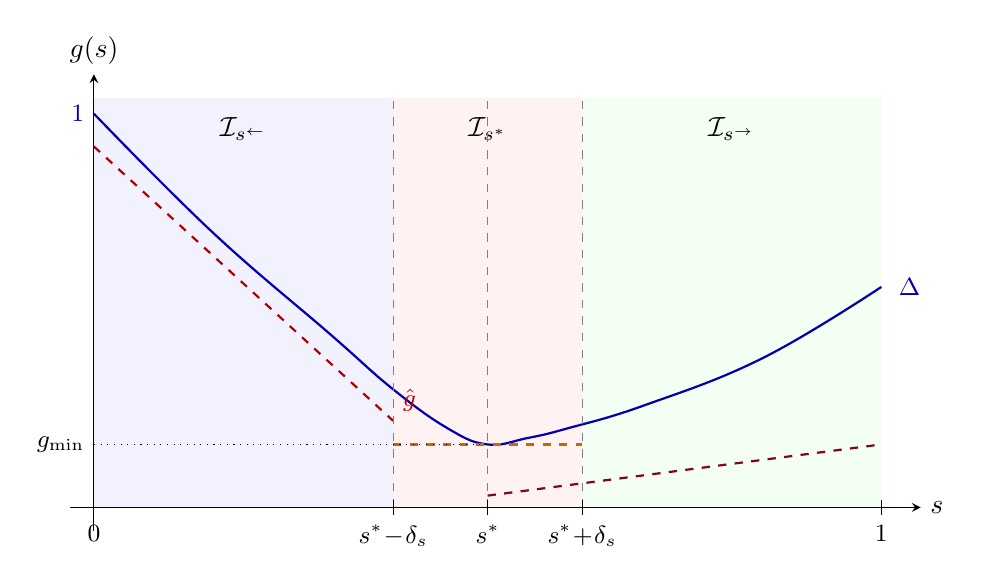
\begin{tikzpicture}[scale=1.0, >=stealth]
  % Axes
  \draw[->] (-0.3,0) -- (10.5,0) node[right] {$s$};
  \draw[->] (0,-0.3) -- (0,5.5) node[above] {$g(s)$};

  % Key positions
  \def\sstar{5.0}
  \def\dsl{1.2}
  \def\dsr{1.2}
  \def\gmin{0.8}
  \def\ghat{1.1}

  % Region shading
  \fill[blue!5] (0,0) rectangle (\sstar-\dsl,5.2);
  \fill[red!5] (\sstar-\dsl,0) rectangle (\sstar+\dsr,5.2);
  \fill[green!5] (\sstar+\dsr,0) rectangle (10,5.2);

  % Region labels
  \node at ({(\sstar-\dsl)/2}, 4.8) {$\mathcal{I}_{s^\leftarrow}$};
  \node at (\sstar, 4.8) {$\mathcal{I}_{s^*}$};
  \node at ({(\sstar+\dsr+10)/2}, 4.8) {$\mathcal{I}_{s^\rightarrow}$};

  % Exact gap (asymmetric: steep left arm, shallow right arm)
  \draw[thick, blue!70!black] plot[smooth, tension=0.7] coordinates {
    (0, 5.0)
    (1.5, 3.5)
    (3.0, 2.2)
    (3.8, 1.5)
    (4.5, 1.0)
    (\sstar, \gmin)
    (5.5, 0.88)
    (6.0, 1.0)
    (7.0, 1.3)
    (8.5, 1.9)
    (10, 2.8)
  };

  % Lower bounds (dashed)
  % Left: g(s) >= A_1(A_1+1)/A_2 * (s*-s), equals g_hat at s*-delta_s
  \draw[dashed, thick, red!70!black] (0, {(\sstar)*\ghat/\dsl}) -- (\sstar-\dsl, \ghat);

  % Window: horizontal at g_min
  \draw[dashed, thick, orange!80!black] (\sstar-\dsl, \gmin) -- (\sstar+\dsr, \gmin);

  % Right: g(s) >= Delta/30 * (s-s_0)/(1-s_0), slope controlled by Delta
  \draw[dashed, thick, purple!70!black] (\sstar, 0.15) -- (10, 0.80);

  % Vertical dashed lines at region boundaries
  \draw[thin, dashed, gray] (\sstar-\dsl, 0) -- (\sstar-\dsl, 5.2);
  \draw[thin, dashed, gray] (\sstar, 0) -- (\sstar, 5.2);
  \draw[thin, dashed, gray] (\sstar+\dsr, 0) -- (\sstar+\dsr, 5.2);

  % Tick marks
  \draw (0, 0.1) -- (0, -0.1) node[below, font=\small] {$0$};
  \draw (\sstar-\dsl, 0.1) -- (\sstar-\dsl, -0.1) node[below, font=\small] {$s^*\!-\!\delta_s$};
  \draw (\sstar, 0.1) -- (\sstar, -0.1) node[below, font=\small] {$s^*$};
  \draw (\sstar+\dsr, 0.1) -- (\sstar+\dsr, -0.1) node[below, font=\small] {$s^*\!+\!\delta_s$};
  \draw (10, 0.1) -- (10, -0.1) node[below, font=\small] {$1$};

  % g_min label
  \draw[thin, dotted] (0, \gmin) -- (\sstar, \gmin);
  \node[left, font=\small] at (0, \gmin) {$g_{\min}$};

  % g_hat label at window boundary
  \node[red!70!black, above right, font=\small] at (\sstar-\dsl, \ghat) {$\hat{g}$};

  % Endpoint values
  \node[blue!70!black, left, font=\small] at (0, 5.0) {$1$};
  \node[blue!70!black, right, font=\small] at (10.1, 2.8) {$\Delta$};
\end{tikzpicture}
\caption{Schematic gap profile for $H(s)$. The solid curve shows the true spectral gap $g(s)$, which equals $1$ at $s=0$, dips to $g_{\min}$ at $s = s^*$, and recovers to $\Delta$ at $s=1$. The left arm is steep (slope $A_1(A_1+1)/A_2$); the right arm is shallower (slope controlled by $\Delta$). Dashed lines show the piecewise lower bounds from \autoref{thm:complete-profile}: linear on the left, constant $g_{\min}$ in the window, and linear on the right (reaching $\Delta/30$ at $s=1$). The right bound is below $g_{\min}$ at $s^*$ but remains $O(g_{\min})$.}
\label{fig:gap-profile}
\end{figure}

Four parameters control the gap: $A_1$, $A_2$, $d_0$, and $\Delta$. For any problem Hamiltonian $H_z$ satisfying the spectral condition, \autoref{thm:complete-profile} bounds $g(s)$ over all of $[0,1]$ up to constants. The minimum is $g_{\min}=\Theta(\sqrt{d_0/(NA_2)})$ at $s^*=A_1/(A_1+1)$, and it is exponentially small in $n$ when $d_0=O(1)$. The crossing location depends only on $A_1$. More solutions (larger $d_0$) widen the gap, while richer near-ground spectral structure (larger $A_2$) narrows it. At $s=1$, the gap returns to $\Delta$, the spectral gap of $H_z$ itself.

For unstructured search, the exact gap $g(s) = \sqrt{(2s-1)^2 + 4s(1-s)/N}$ and the piecewise bound from \autoref{thm:complete-profile} can be compared directly. The left bound has slope $(2N-1)/N \approx 2$, matching the asymptotic slope of the exact gap, which approaches $2(1-1/N) \approx 2$ away from $s^*$. The window bound $g_{\min} = 1/\sqrt{N}$ is exact. The right bound has slope approximately $1/15$ near $s^*$, weaker than the true slope by a factor of $30$, but sufficient for the runtime integral since the window dominates.

The window dominates the runtime integral. $\int_0^1 g(s)^{-2}\,ds$ splits across the three regions. In the left and right regions, $g(s) \sim C|s - s^*|$ for constants $C$, and
\begin{equation}
\int_{\delta_s}^{s^*} \frac{du}{(Cu)^2} = \frac{1}{C^2}\left(\frac{1}{\delta_s} - \frac{1}{s^*}\right) \leq \frac{1}{C^2\delta_s},
\end{equation}
which is $O(1/(C^2\delta_s))$. In the window, $g(s) \geq g_{\min}$ gives $\int_{s^*-\delta_s}^{s^*+\delta_s} g(s)^{-2}\,ds \leq 2\delta_s/g_{\min}^2$. The window contribution $\delta_s/g_{\min}^2 = \Theta(A_2^{3/2}/(A_1(A_1+1)) \cdot \sqrt{N/d_0})$ dominates the outer regions. Once the $\Delta$-dependent right-arm term is included, the full integral yields the runtime
\[
T = O\!\left(\frac{\sqrt{A_2}}{A_1(A_1+1)\Delta^2}\sqrt{\frac{N}{d_0}}\right),
\]
which Chapter 7 derives rigorously.


\chapter{Optimal Schedule}
% Chapter 7: Optimal Schedule
% ASSUMES: Chapter 4 defines AQC, adiabatic theorem, spectral gap as
%   computational resource, avoided crossings, local/adaptive schedules,
%   Roland-Cerf construction.
% ASSUMES: Chapter 5 defines H(s), H_z, H_0, |psi_0>, A_p, A_1, A_2,
%   s^*, delta_s, g_min, hat{g}, the three regions, eigenvalue equation,
%   spectral condition (Definition 5.x), grover-gap.
% ASSUMES: Chapter 6 proves gap-left (Lemma 6.1), gap-right (Lemma 6.2),
%   complete-profile (Theorem 6.x), f(s*) = 4, s_0 formula.

The spectral gap of $H(s)$ is now bounded from below on all of $[0,1]$.
\autoref{thm:complete-profile} shows a piecewise form. The gap reaches
$g_{\min}$ at $s^*$, then reopens with slope $A_1(A_1+1)/A_2$ on the left and
$\Delta/30$ on the right. Chapter 5 already identified the key runtime integral,
$\int_0^1 g(s)^{-2}\,ds$ (Eq.~\eqref{eq:runtime-integral-preview}), and showed
that the crossing window dominates. The remaining issue is the adiabatic
theorem itself. Its error bound determines which power of $g$ controls runtime.

With a constant-rate theorem, runtime is controlled by
$\int_0^1 g(s)^{-3}\,ds$. For the profile of \autoref{thm:complete-profile},
the crossing window contributes $\delta_s/g_{\min}^3$. In the two-level case
$M = 2$ with $g_{\min} = 1/\sqrt{N}$, this gives $T = O(N)$ and no speedup over
classical search. An adaptive schedule with $K'(s)$ scaled to the gap replaces
$\int g^{-3}\,ds$ with $\int g^{-p}\,ds$ for $p \in (1,2)$. The resulting
runtime
\[
T = O\!\left(\frac{\sqrt{A_2}}{A_1(A_1+1)\Delta^2}\sqrt{\frac{N}{d_0}}\frac{1}{\varepsilon}\right)
\]
matches Grover scaling up to explicit spectral prefactors.

\section{How Theorem Choice Sets Runtime}
\label{sec:prior-theorems}

The gap profile alone does not determine runtime. Translating spectral data into evolution time requires an adiabatic theorem, and different theorems permit different schedules. That choice changes the gap dependence and, in the running example, is exactly the difference between $O(N)$ and $O(\sqrt{N})$.

The earliest rigorous bounds, due to Jansen, Ruskai, and
Seiler~\cite{jansen2007bounds}, apply to a constant schedule $K'(s) = T$ and
give a transition probability of order $O(1/T^2)$. Their Theorem~3 states that
for a state $\psi \in P(0)$, the probability of leaving the ground space
satisfies
\begin{equation}
\label{eq:jrs-bound}
(\psi, [1-P(s)]U_\tau(s)\psi) \leq A(s)^2,
\end{equation}
where
$A(s) \leq (1/T)(\lVert H' \rVert/g^2)\vert_{\mathrm{bdry}}
+ (1/T)\int_0^s (7\sqrt{m}\,\lVert H'\rVert^2/g^3 + \lVert H'\rVert/g^2)\,ds'$,
with $m$ the multiplicity of the ground eigenvalue and the boundary term
evaluated at $s = 0$ and $s$. Setting $A(s) = \varepsilon$ and solving for $T$
gives
\begin{equation}
\label{eq:jrs-runtime}
T = O\!\left(\frac{1}{\varepsilon}\int_0^1 \frac{\lVert H'\rVert^2}{g(s)^3}\,ds\right).
\end{equation}
With $M = 2$ and $\lVert H'\rVert = O(1)$, the integral $\int_0^1 g^{-3}\,ds$
is dominated by the $O(1/\sqrt{N})$-wide window where $g \approx 1/\sqrt{N}$.
Its contribution is $(1/\sqrt{N})\cdot N^{3/2} = N$. Therefore the JRS bound
gives $T = O(N/\varepsilon)$, which matches classical search. A constant
schedule allocates the same physical time per unit of $s$ whether the gap is
$O(1)$ or $O(1/\sqrt{N})$. That uniform allocation forces the $g^{-3}$
dependence, so the narrow crossing window dominates and the quantum speedup
disappears.

The resolution is to let the schedule depend on the gap. Roland and Cerf~\cite{roland2002quantum} introduced a \emph{local} adiabatic condition. Instead of enforcing adiabaticity with one global timescale $T$, they enforce it infinitesimally on each segment $[s,s+ds]$. The standard criterion gives
\[
\left|\frac{ds}{dt}\right| \leq \frac{\varepsilon\, g(s)^2}{|\langle e_1(s)|H'(s)|e_0(s)\rangle|},
\]
where $e_0,e_1$ are the ground and first excited states. Inverting this inequality yields
\[
K'(s)=\frac{dt}{ds}\geq \frac{|\langle e_1|H'|e_0\rangle|}{\varepsilon\,g(s)^2}.
\]
For the running example, $|\langle e_1|H'|e_0\rangle|=O(1)$ because $H'(s)=\ket{\psi_0}\bra{\psi_0}+H_z$ is constant. Thus $K'(s)\propto 1/g(s)^2$, and the runtime becomes
\begin{equation}
\label{eq:roland-cerf-runtime}
T = \frac{C}{\varepsilon}\int_0^1 g(s)^{-2}\,ds.
\end{equation}
The integral can be evaluated explicitly. Writing $g(s)^2 = (2s-1)^2 + 4s(1-s)/N$ and substituting $u = 2s - 1$:
\begin{equation}
\label{eq:roland-cerf-integral}
\int_0^1 g(s)^{-2}\,ds = \frac{1}{2}\int_{-1}^{1}\frac{du}{u^2 + (1-u^2)/N} = \frac{1}{2}\int_{-1}^{1}\frac{N\,du}{1 + (N-1)u^2}.
\end{equation}
For large $N$, the substitution $v = \sqrt{N-1}\,u$ gives $\frac{N}{2\sqrt{N-1}}\int_{-\sqrt{N-1}}^{\sqrt{N-1}}\frac{dv}{1+v^2} = \frac{N}{2\sqrt{N-1}}\cdot 2\arctan(\sqrt{N-1}) = O(\sqrt{N})$, since $\arctan(\sqrt{N-1}) \to \pi/2$. Therefore $T = O(\sqrt{N}/\varepsilon)$, recovering the Grover speedup from a smooth, continuous-time evolution.

The Roland-Cerf construction requires exact knowledge of $g(s)$ at every point. For the running example with $M=2$, this is feasible because the gap has the closed form in Eq.~\eqref{eq:grover-gap}. For a general $M$-level problem Hamiltonian, the exact gap is unknown and only the piecewise bounds of \autoref{thm:complete-profile} are available. If one substitutes a lower bound $g_0(s)\le g(s)$, the schedule slows down conservatively because $1/g_0^2 \ge 1/g^2$, so the runtime increases only by constants. The difficulty shifts to error control: derivative terms in the adiabatic bound become sensitive to corners in $g_0$. The adaptive schedule of \autoref{sec:adaptive-schedule} addresses this through the exponent $p\in(1,2)$.

Several later results sharpened this picture. Boixo, Knill, and
Somma~\cite{boixo2009eigenpath} introduced eigenpath traversal, which replaces
continuous evolution with projections onto ground states of intermediate
Hamiltonians $H(s_0),H(s_1),\ldots,H(s_L)$. Their key ingredient is phase
randomization between steps. It suppresses coherent accumulation of diabatic
error, which otherwise recreates the usual $O(1/g_{\min}^2)$ behavior. Under
that phase randomization, coherent errors from successive transitions no longer
add constructively.
Under the condition $\int g^{-p}\,ds = O(g_{\min}^{1-p})$, this gives
$O(1/g_{\min})$ scaling. Cunningham and Roland~\cite{cunningham2024eigenpath}
tightened constants and gave a continuous-time version that underlies
\autoref{sec:error-bound}. Elgart and Hagedorn~\cite{ElgartHagedorn2012}
followed a different route using Gevrey-smooth switching, obtaining
superpolynomial suppression with runtime
$T \geq K\, g^{-2}\lvert\ln g\rvert^{6\alpha}$. The schedule used here has a
different practical advantage: it only needs a certified lower bound
$g_0(s)\le g(s)$, not the exact gap.

\section{The Adiabatic Error Bound}
\label{sec:error-bound}

The Schr\"odinger equation $i\,d\ket{\psi}/dt = H(s(t))\ket{\psi}$ governs the evolution under the time-dependent Hamiltonian $H(s)$, with $s:[0,T]\to[0,1]$ parameterizing the interpolation. The density-matrix form $d\rho/dt=-i[H,\rho]$ is more convenient for the error analysis and also covers mixed states. We reparameterize time by $t=K(s)$, where $K:[0,1]\to\mathbb{R}^+$ is differentiable and monotone increasing. The chain rule then gives
\begin{equation}
\label{eq:reparametrized-evolution}
\frac{d\rho}{ds} = -iK'(s)[H(s), \rho(s)],
\end{equation}
where $K'(s) = dK/ds > 0$ controls the instantaneous evolution rate. The total runtime is $T = K(1) = \int_0^1 K'(s)\,ds$. A large $K'(s)$ means slow evolution (long physical time per unit of $s$), allowing the state to track the ground state through a small-gap region. A small $K'(s)$ means fast evolution, appropriate where the gap is large and diabatic transitions are suppressed.

The error of the adiabatic evolution is the probability that the final state does not lie in the ground space of $H(1)$:
\begin{equation}
\label{eq:error-def}
\varepsilon = 1 - \mathrm{Tr}[P(1)\rho(1)],
\end{equation}
where $P(s)$ denotes the projector onto the ground eigenspace of $H(s)$ and $\rho(0) = P(0)$ (the system starts in the ground state of $H(0)$). The projector $P(s)$ and the ground energy $\lambda_0(s)$ are both functions of $s$, varying as the Hamiltonian interpolates from $H_0$ to $H_z$. The operator
\begin{equation}
\label{eq:pseudoinverse-def}
(H(s) - \lambda_0(s))^+ = \sum_{j \geq 1} \frac{1}{\lambda_j(s) - \lambda_0(s)}\,\ket{\phi_j(s)}\bra{\phi_j(s)}
\end{equation}
is the pseudoinverse of $H(s) - \lambda_0(s)$: it acts as zero on the ground space and as $(\lambda_j - \lambda_0)^{-1}$ on the $j$-th excited eigenspace. Its operator norm is $1/g(s)$, so a small spectral gap amplifies the pseudoinverse.

\begin{lemma}[Adiabatic error bound {\cite{braida2024unstructured, cunningham2024eigenpath}}]
\label{lem:error-bound}
Let $H(s)$ be a twice-differentiable path of Hamiltonians with a continuous ground energy $\lambda_0(s)$ and a spectral gap $g(s) > 0$ for all $s \in [0,1]$. Let $K: [0,1] \to \mathbb{R}^+$ be a schedule with absolutely continuous derivative $K'$. Then the evolution~\eqref{eq:reparametrized-evolution} starting from $\rho(0) = P(0)$ satisfies
\begin{equation}
\label{eq:error-bound}
\varepsilon \leq \frac{1}{K'(1)}\left\lVert\left[P'(1),\, (H(1) - \lambda_0(1))^+\right]\right\rVert + \int_0^1 \frac{1}{K'}\left\lVert\left[P',\, (H - \lambda_0)^+\right]'\right\rVert ds + \int_0^1 \left|\left(\frac{1}{K'}\right)'\right|\left\lVert\left[P',\, (H - \lambda_0)^+\right]\right\rVert ds.
\end{equation}
\end{lemma}

\begin{proof}
Since $\rho(0) = P(0)$, the error is $\varepsilon = \mathrm{Tr}[P(0)\rho(0)] - \mathrm{Tr}[P(1)\rho(1)] = \left|\mathrm{Tr}[P\rho]\right|_0^1$, so it suffices to track $\mathrm{Tr}[P(s)\rho(s)]$. Differentiating:
\begin{equation}
\frac{d}{ds}\mathrm{Tr}[P\rho] = \mathrm{Tr}[P'\rho] + \mathrm{Tr}[P\rho'].
\end{equation}
The second term vanishes. Substituting the evolution equation~\eqref{eq:reparametrized-evolution}: $\mathrm{Tr}[P\rho'] = -iK'\,\mathrm{Tr}[P[H,\rho]]$. Since $HP = \lambda_0 P$, the cyclic property gives $\mathrm{Tr}[P[H,\rho]] = \mathrm{Tr}[PH\rho - P\rho H] = \lambda_0\,\mathrm{Tr}[P\rho] - \mathrm{Tr}[HP\rho] = 0$.

For $\mathrm{Tr}[P'\rho]$, write $Q = I - P$ and use the decomposition $P' = PP'Q + QP'P$, which holds because $PP'P = 0$ and $QP'Q = 0$.\footnote{Differentiating $P^2 = P$ gives $P'P + PP' = P'$. Left-multiplying by $P$: $PP'P + PP' = PP'$, so $PP'P = 0$. Then $QP'Q = P' - PP' - P'P + PP'P = P' - P' = 0$.} Inserting $Q = (H-\lambda_0)^+(H-\lambda_0)$ and using the identities $(H-\lambda_0)\rho P = [H,\rho]P$ and $P\rho(H-\lambda_0) = -P[H,\rho]$ (both consequences of $HP = \lambda_0 P$), a cyclic rearrangement under the trace gives
\begin{equation}
\mathrm{Tr}[P'\rho] = \mathrm{Tr}\!\left[PP'(H-\lambda_0)^+[H,\rho]\right] - \mathrm{Tr}\!\left[(H-\lambda_0)^+P'P[H,\rho]\right].
\end{equation}
Since $(H-\lambda_0)^+P = P(H-\lambda_0)^+ = 0$ (the pseudoinverse annihilates the ground space), $PP'(H-\lambda_0)^+$ reduces to $P'(H-\lambda_0)^+$ and $(H-\lambda_0)^+P'P$ reduces to $(H-\lambda_0)^+P'$, so the two terms combine into a commutator:
\begin{equation}
\mathrm{Tr}[P'\rho] = \mathrm{Tr}\!\left[\left[P',\, (H-\lambda_0)^+\right][H,\rho]\right] = i(K')^{-1}\,\mathrm{Tr}\!\left[\left[P',\, (H-\lambda_0)^+\right]\rho'\right],
\end{equation}
where the last equality substitutes $[H,\rho] = i(K')^{-1}\rho'$ from~\eqref{eq:reparametrized-evolution}.

Integrating from $0$ to $1$ gives $\mathrm{Tr}[P\rho]\big|_0^1 = i\int_0^1 (K')^{-1}\,\mathrm{Tr}\!\left[\left[P',\, (H-\lambda_0)^+\right]\rho'\right]ds$. Integration by parts, with $u = (K')^{-1}[P',\,(H-\lambda_0)^+]$ and $dv = \rho'\,ds$, transfers the derivative from $\rho$ onto $u$:
\begin{multline}
\mathrm{Tr}[P\rho]\big|_0^1 = i(K'(1))^{-1}\,\mathrm{Tr}\!\left[\left[P'(1),\, (H(1)-\lambda_0(1))^+\right]\rho(1)\right] \\
- i\int_0^1 \mathrm{Tr}\!\left[\left((K')^{-1}\left[P',\, (H-\lambda_0)^+\right]' + \left((K')^{-1}\right)'\!\left[P',\, (H-\lambda_0)^+\right]\right)\rho\right]ds.
\end{multline}
The boundary term at $s = 0$ vanishes. Since $\rho(0) = P(0)$, the commutator trace expands as
\[
\mathrm{Tr}\!\left[\left[P',\,(H-\lambda_0)^+\right]P\right] = \mathrm{Tr}[P'(H-\lambda_0)^+P] - \mathrm{Tr}[(H-\lambda_0)^+P'P].
\]
For the first summand, $(H-\lambda_0)^+P = 0$ (the pseudoinverse annihilates the ground-space projector), so $\mathrm{Tr}[P'(H-\lambda_0)^+P] = 0$. For the second, cyclicity of the trace gives $\mathrm{Tr}[(H-\lambda_0)^+P'P] = \mathrm{Tr}[P(H-\lambda_0)^+P'] = 0$ by the same identity. Taking absolute values and bounding $|\mathrm{Tr}[A\rho]| \leq \lVert A\rVert$ for any density matrix $\rho$ yields~\eqref{eq:error-bound}.
\end{proof}

The error bound depends on $H(s)$ only through the commutator $[P', (H-\lambda_0)^+]$ and its derivative. The following bounds express these in terms of the Hamiltonian derivatives $H'$, $H''$ and the spectral gap $g$, using the Riesz integral representation of the spectral projector introduced by Kato~\cite{Kato1950}.

\begin{lemma}[Projector derivative bounds {\cite{braida2024unstructured}}]
\label{lem:derivative-bounds}
Under the conditions of \autoref{lem:error-bound}:
\begin{align}
\label{eq:P-prime-bound}
\lVert P'(s) \rVert &\leq \frac{2\lVert H'(s)\rVert}{g(s)}, \\
\label{eq:commutator-bound}
\left\lVert\left[P'(s),\, (H(s) - \lambda_0(s))^+\right]\right\rVert &\leq \frac{4\lVert H'(s)\rVert}{g(s)^2}, \\
\label{eq:commutator-deriv-bound}
\left\lVert\left[P'(s),\, (H(s) - \lambda_0(s))^+\right]'\right\rVert &\leq \frac{40\lVert H'(s)\rVert^2}{g(s)^3} + \frac{4\lVert H''(s)\rVert}{g(s)^2}.
\end{align}
\end{lemma}

\begin{proof}[Proof of~\eqref{eq:P-prime-bound}]
Let $\Gamma$ be a circle in the complex plane centered at $\lambda_0(s)$ with radius $g(s)/2$. The Riesz integral representation gives
\begin{equation}
P(s) = \frac{1}{2\pi i}\oint_\Gamma R_{H(s)}(z)\,dz,
\end{equation}
where $R_{H(s)}(z) = (zI - H(s))^{-1}$ is the resolvent. Differentiating with respect to $s$:
\begin{equation}
P'(s) = \frac{1}{2\pi i}\oint_\Gamma R_{H(s)}(z)\,H'(s)\,R_{H(s)}(z)\,dz,
\end{equation}
using the resolvent identity $R_H' = R_H H' R_H$. On the contour $\Gamma$, every point $z$ lies at distance exactly $g(s)/2$ from $\lambda_0(s)$ and at distance at least $g(s)/2$ from every other eigenvalue (since the nearest eigenvalue is $\lambda_1(s)$ at distance $g(s)$ from $\lambda_0(s)$). Therefore $\lVert R_{H(s)}(z) \rVert = 1/\mathrm{dist}(z, \sigma(H(s))) \leq 2/g(s)$ on $\Gamma$. Bounding the integral:
\begin{equation}
\lVert P'(s) \rVert \leq \frac{1}{2\pi}\oint_\Gamma \lVert R_H(z)\rVert \cdot \lVert H'(s)\rVert \cdot \lVert R_H(z)\rVert\,|dz| \leq \frac{1}{2\pi}\left(\frac{2}{g}\right)^2\lVert H'\rVert \cdot \pi g = \frac{2\lVert H'\rVert}{g}.
\end{equation}
\end{proof}

Bound~\eqref{eq:commutator-bound} follows from~\eqref{eq:P-prime-bound}: $\lVert[A,B]\rVert \leq 2\lVert A\rVert\cdot\lVert B\rVert$ gives $\lVert[P', (H-\lambda_0)^+]\rVert \leq 2 \cdot 2\lVert H'\rVert/g \cdot 1/g = 4\lVert H'\rVert/g^2$.

Bound~\eqref{eq:commutator-deriv-bound} requires two intermediate results. Write $\widetilde{H} = H - \lambda_0$ for the shifted Hamiltonian. Its pseudoinverse satisfies
\begin{equation}
\label{eq:pseudoinverse-derivative}
(\widetilde{H}^+)' = -\widetilde{H}^+\widetilde{H}'\widetilde{H}^+ + P'\widetilde{H}^+ + \widetilde{H}^+P',
\end{equation}
where $\widetilde{H}' = H' - \lambda_0'$. To see this, split the difference quotient $(\widetilde{H}^+(s+h) - \widetilde{H}^+(s))/h$ using $Q = \widetilde{H}^+\widetilde{H}$ and $P = I - Q$. The $Q$-part gives $\lim_{h\to 0}\widetilde{H}^+(s)(\widetilde{H}(s) - \widetilde{H}(s+h))\widetilde{H}^+(s+h)/h = -\widetilde{H}^+\widetilde{H}'\widetilde{H}^+$, while the $P$-part, after adding and subtracting $P(s+h)\widetilde{H}^+(s+h)$ and $\widetilde{H}^+(s)P(s)$, yields $P'\widetilde{H}^+ + \widetilde{H}^+P'$. Bounding the norm and using $|\lambda_0'| = |\langle\phi_0|H'|\phi_0\rangle| \leq \lVert H'\rVert$ (Hellmann-Feynman):
\begin{equation}
\label{eq:pseudoinverse-deriv-bound}
\lVert(\widetilde{H}^+)'\rVert \leq \frac{\lVert H'\rVert + |\lambda_0'|}{g^2} + \frac{4\lVert H'\rVert}{g^2} \leq \frac{6\lVert H'\rVert}{g^2}.
\end{equation}

The second intermediate result bounds $P''$. Differentiating $P' = (2\pi i)^{-1}\oint_\Gamma R_H H' R_H\,dz$ gives
\begin{equation}
P'' = \frac{1}{2\pi i}\oint_\Gamma \left(2R_H H' R_H H' R_H + R_H H'' R_H\right)dz,
\end{equation}
where the two $R_H H' R_H H' R_H$ terms arise from differentiating each resolvent factor. Bounding by $\lVert R_H(z)\rVert \leq 2/g$ on $\Gamma$ and integrating over the contour of length $\pi g$:
\begin{equation}
\label{eq:P-double-prime-bound}
\lVert P''\rVert \leq \frac{1}{2\pi}\left(\frac{2}{g}\right)^{\!3}\!2\lVert H'\rVert^2 \cdot \pi g + \frac{1}{2\pi}\left(\frac{2}{g}\right)^{\!2}\!\lVert H''\rVert \cdot \pi g = \frac{8\lVert H'\rVert^2}{g^2} + \frac{2\lVert H''\rVert}{g}.
\end{equation}

Now expand $[P', (H-\lambda_0)^+]' = [P'', (H-\lambda_0)^+] + [P', ((H-\lambda_0)^+)']$ and bound each commutator:
\begin{equation}
\lVert[P'', (H-\lambda_0)^+]\rVert \leq \frac{2\lVert P''\rVert}{g} \leq \frac{16\lVert H'\rVert^2}{g^3} + \frac{4\lVert H''\rVert}{g^2},
\end{equation}
and, using~\eqref{eq:P-prime-bound} and~\eqref{eq:pseudoinverse-deriv-bound}:
\begin{equation}
\lVert[P', ((H-\lambda_0)^+)']\rVert \leq 2\lVert P'\rVert\cdot\lVert(\widetilde{H}^+)'\rVert \leq 2\cdot\frac{2\lVert H'\rVert}{g}\cdot\frac{6\lVert H'\rVert}{g^2} = \frac{24\lVert H'\rVert^2}{g^3}.
\end{equation}
Summing gives $40\lVert H'\rVert^2/g^3 + 4\lVert H''\rVert/g^2$. A block-matrix decomposition of the commutator with respect to $P$ and $Q = I - P$, tracking cross terms exactly rather than using submultiplicativity, replaces the coefficient $40$ by $\approx 4.77$ \cite{braida2024unstructured}; the asymptotic scaling is unchanged.

The simplest schedule is constant. It sets $K'(s) = T$, so evolution proceeds at a uniform rate regardless of the gap. Substituting the derivative bounds into the error bound~\eqref{eq:error-bound} with $(1/K')' = 0$ gives the constant-rate result.

\begin{theorem}[Constant-rate runtime]
\label{thm:constant-rate}
Under the conditions of \autoref{lem:error-bound}, a constant schedule $K'(s) = T$ achieves error at most $\varepsilon$ provided
\begin{equation}
\label{eq:constant-rate-formula}
T \geq \frac{1}{\varepsilon}\left(\frac{4\lVert H'(1)\rVert}{g(1)^2} + \int_0^1 \frac{40\lVert H'(s)\rVert^2}{g(s)^3}\,ds + \int_0^1\frac{4\lVert H''(s)\rVert}{g(s)^2}\,ds\right).
\end{equation}
\end{theorem}

\begin{proof}
With constant $K'$, the third term in~\eqref{eq:error-bound} vanishes. Substituting bounds~\eqref{eq:commutator-bound} and~\eqref{eq:commutator-deriv-bound} into the remaining two terms:
\begin{equation}
\varepsilon \leq \frac{1}{T}\left(\frac{4\lVert H'(1)\rVert}{g(1)^2} + \int_0^1 \frac{40\lVert H'(s)\rVert^2}{g(s)^3}\,ds + \int_0^1\frac{4\lVert H''(s)\rVert}{g(s)^2}\,ds\right).
\end{equation}
Setting the right side equal to $\varepsilon$ and solving for $T$ gives~\eqref{eq:constant-rate-formula}.
\end{proof}

Since $H'' = 0$ for the linear interpolation $H(s) = -(1-s)\ket{\psi_0}\bra{\psi_0} + sH_z$, and $H'(s) = \ket{\psi_0}\bra{\psi_0} + H_z$ is constant with $\lVert H'\rVert = O(1)$, the dominant term in~\eqref{eq:constant-rate-formula} is $\int_0^1 g(s)^{-3}\,ds$. From the gap profile of \autoref{thm:complete-profile}, the crossing window contributes
\begin{equation}
\label{eq:constant-rate-window}
\int_{s^*-\delta_s}^{s^*} g(s)^{-3}\,ds \leq \frac{\delta_s}{g_{\min}^3} = \frac{A_2}{A_1(A_1+1)}\cdot g_{\min}^{-2},
\end{equation}
using $\delta_s = A_2 g_{\min}/(A_1(A_1+1))$ from Eq.~\eqref{eq:gmin-deltas-relation}. This gives $T_{\mathrm{constant}} = O(\delta_s/(\varepsilon\, g_{\min}^3))$.

Specializing to $M=2$ with $g_{\min}=1/\sqrt{N}$, the exact gap $g(s)=\sqrt{(2s-1)^2+4s(1-s)/N}$ from Eq.~\eqref{eq:grover-gap} gives $\int_0^1 g(s)^{-3}\,ds = O(N)$. The dominant contribution comes from the $O(1/\sqrt{N})$ window where $g\approx 1/\sqrt{N}$. Hence $T_{\mathrm{constant}}=O(N/\varepsilon)$, matching classical search. A constant-rate schedule therefore gives no quantum speedup. It wastes time where the gap is large and still moves too quickly near $s^*$.

\section{The Adaptive Schedule}
\label{sec:adaptive-schedule}

The constant schedule fails because it treats every value of $s$ the same. The
error bound~\eqref{eq:error-bound} suggests the opposite strategy. Choose large
$K'(s)$ where the gap is small and small $K'(s)$ where the gap is large. Since
$K'(s)=dt/ds$, this means spending physical time where diabatic transitions are
dangerous. The natural ansatz is $K'(s)\propto 1/g(s)^p$ for some $p\ge 1$.
Then runtime scales as $T\propto\int_0^1 g(s)^{-p}\,ds$, while the error terms
involve integrals of the form $\int g^{q-3}\,ds$.

The exponent $p$ controls the runtime-error tradeoff. The family
$K'(s)\propto 1/g_0(s)^p$ extends Roland-Cerf ($p=2$) to a continuum of
schedules. At $p=1$, $\int g_0^{-1}\,ds$ is mild but the companion error
integral $\int g_0^{-2}\,ds$ diverges for piecewise linear profiles. At $p=2$,
the scaling is favorable, but the schedule-variation term requires exact gap
information. The useful regime is therefore $p\in(1,2)$. There,
$\int g_0^{-p}\,ds = O(g_{\min}^{1-p})$ and
$\int g_0^{p-3}\,ds = O(g_{\min}^{p-2})$, whose product is always
$O(g_{\min}^{-1})$. This is exactly the range where a certified lower bound
$g_0\le g$ suffices.

The adaptive rate theorem, extending the eigenpath traversal framework of \cite{cunningham2024eigenpath} to the continuous-time setting, formalizes this trade-off.

\begin{theorem}[Adaptive rate {\cite{braida2024unstructured}}]
\label{thm:adaptive-rate}
Let $H(s)$ satisfy the conditions of \autoref{lem:error-bound}, and let $g_0: [0,1] \to \mathbb{R}^+$ be an absolutely continuous function satisfying $g_0(s) \leq g(s)$ for all $s$. Suppose there exist $1 < p < 2$ (the endpoints are excluded: at $p = 1$ the $B_1$ integral diverges logarithmically, and at $p = 2$ the schedule variation term requires the exact gap) and constants $B_1, B_2 \geq 1$ such that
\begin{equation}
\label{eq:B1-condition}
\int_0^1 \frac{ds}{g_0(s)^p} \leq B_1\, g_{\min}^{1-p} \qquad \text{and} \qquad \int_0^1 \frac{ds}{g_0(s)^{3-p}} \leq B_2\, g_{\min}^{p-2}.
\end{equation}
Assume additionally that $g_0(1) \geq g_{\min}$, that there exists $b \in (0,1]$ with $g_0(s) \geq b\, g_{\min}$ for all $s \in [0,1]$, and that $\sup_{s \in [0,1]} |g_0'(s)| < \infty$.
Define
\begin{equation}
\label{eq:c-constant}
c = \sup_{s \in [0,1]}\left(4\lVert H'(s)\rVert + 40\lVert H'(s)\rVert^2 B_2 + 4\lVert H''(s)\rVert + 6p\,|g_0'(s)|\,\lVert H'(s)\rVert\, B_2\right).
\end{equation}
The last term uses $|g_0'(s)|$ rather than $|g'(s)|$: since the schedule is defined in terms of $g_0$, the derivative $(K'^{-1})' \propto (g_0^p)'$ involves $g_0'$. Then the schedule
\begin{equation}
\label{eq:adaptive-schedule}
K'(s) = \frac{1}{\varepsilon}\cdot\frac{c}{g_0(s)^p \cdot g_{\min}^{2-p}}
\end{equation}
achieves error at most $\varepsilon$, with total runtime
\begin{equation}
\label{eq:adaptive-runtime}
T = \int_0^1 K'(s)\,ds \leq \frac{c\, B_1}{\varepsilon\, g_{\min}}.
\end{equation}
\end{theorem}

\begin{proof}
Let $\varepsilon_0$ denote the actual error. Substituting~\eqref{eq:adaptive-schedule} into the error bound~\eqref{eq:error-bound}: $(K')^{-1} = \varepsilon\, g_0^p\, g_{\min}^{2-p}/c$, and $|((K')^{-1})'| = (\varepsilon\, g_{\min}^{2-p}/c)\cdot p\, g_0^{p-1}\,|g_0'|$. The three terms become
\begin{multline}
\label{eq:adaptive-error-expanded}
\varepsilon_0 \leq \frac{\varepsilon}{c}\, g_{\min}^{2-p}\biggl(g_0(1)^p\left\lVert\left[P'(1), (H(1)-\lambda_0(1))^+\right]\right\rVert \\
+ \int_0^1 g_0^p\left\lVert\left[P', (H-\lambda_0)^+\right]'\right\rVert ds + \int_0^1 p\, g_0^{p-1}|g_0'|\left\lVert\left[P', (H-\lambda_0)^+\right]\right\rVert ds\biggr).
\end{multline}

\textbf{Boundary term.} Using bound~\eqref{eq:commutator-bound} with $g_0 \leq g$:
\begin{equation}
g_{\min}^{2-p}\, g_0(1)^p \cdot \frac{4\lVert H'(1)\rVert}{g(1)^2} \leq 4\lVert H'(1)\rVert\, g_{\min}^{2-p}\, g_0(1)^{p-2} \leq 4\lVert H'\rVert,
\end{equation}
since $g_0(1) \geq g_{\min}$ and $p - 2 < 0$ imply $g_0(1)^{p-2} \leq g_{\min}^{p-2}$.

\textbf{Commutator derivative integral.} Using bound~\eqref{eq:commutator-deriv-bound} and splitting:
\begin{align}
g_{\min}^{2-p}\int_0^1 g_0^p \cdot \frac{40\lVert H'\rVert^2}{g^3}\,ds &\leq 40\lVert H'\rVert^2\, g_{\min}^{2-p}\int_0^1 \frac{ds}{g_0^{3-p}} \leq 40\lVert H'\rVert^2 B_2, \label{eq:proof-term-H-prime}
\end{align}
where $g_0^p/g^3 \leq g_0^p/g_0^3 = 1/g_0^{3-p}$ since $g_0 \leq g$, and the $B_2$ condition~\eqref{eq:B1-condition} absorbs $g_{\min}^{2-p}\cdot g_{\min}^{p-2} = 1$. Similarly, the $H''$ sub-term contributes
\begin{equation}
g_{\min}^{2-p}\int_0^1 g_0^p \cdot \frac{4\lVert H''\rVert}{g^2}\,ds \leq 4\lVert H''\rVert\, g_{\min}^{2-p}\int_0^1 \frac{ds}{g_0^{2-p}} \leq 4\lVert H''\rVert, \label{eq:proof-term-H-double-prime}
\end{equation}
since $g_0 \geq b\, g_{\min}$ and $p - 2 < 0$ imply $g_0^{p-2} \leq b^{p-2} g_{\min}^{p-2}$, giving $\int g_0^{p-2}\,ds = O(g_{\min}^{p-2})$ with the constant $b^{p-2}$ absorbed into the $O$-notation.

\textbf{Schedule variation integral.} Using bound~\eqref{eq:commutator-bound}:
\begin{align}
g_{\min}^{2-p}\int_0^1 p\, g_0^{p-1}|g_0'| \cdot \frac{4\lVert H'\rVert}{g^2}\,ds &\leq 4p\,\lVert H'\rVert\, g_{\min}^{2-p}\int_0^1 \frac{g_0^{p-1}\,|g_0'|}{g_0^2}\,ds \nonumber \\
&= 4p\,\lVert H'\rVert\, g_{\min}^{2-p}\int_0^1 g_0^{p-3}\,|g_0'|\,ds. \label{eq:proof-schedule-variation}
\end{align}
Using $\sup|g_0'| < \infty$, we have $\int g_0^{p-3}|g_0'|\,ds \leq \sup|g_0'|\cdot \int g_0^{p-3}\,ds \leq \sup|g_0'|\cdot B_2\, g_{\min}^{p-2}$. The resulting bound is $4p\,\sup|g_0'|\,\lVert H'\rVert\, B_2$. The constant $c$ in~\eqref{eq:c-constant} uses the factor $6p$ rather than $4p$; this is a valid overestimate that simplifies the expression without affecting the asymptotic result.

\textbf{Collecting.} Summing all contributions:
\begin{equation}
\varepsilon_0 \leq \frac{\varepsilon}{c}\left(4\lVert H'\rVert + 40\lVert H'\rVert^2 B_2 + 4\lVert H''\rVert + 6p\,\sup|g_0'|\,\lVert H'\rVert\, B_2\right) \leq \frac{\varepsilon}{c}\cdot c = \varepsilon.
\end{equation}

\textbf{Runtime.} The total evolution time is
\begin{equation}
T = \int_0^1 K'\,ds = \frac{c}{\varepsilon}\, g_{\min}^{p-2}\int_0^1 \frac{ds}{g_0^p} \leq \frac{c}{\varepsilon}\, g_{\min}^{p-2}\cdot B_1\, g_{\min}^{1-p} = \frac{c\, B_1}{\varepsilon\, g_{\min}}. \qedhere
\end{equation}
\end{proof}

Three terms compose the error. The first is a boundary term that depends on $g_0(1)$ and is $O(1)$. The second is an integral that pairs $g_0^p$ from the schedule with $g^{-3}$ from the derivative bounds, producing $\int g_0^{p-3}\,ds$. The third is a schedule-variation term from the non-constant $K'$. The parameter $p$ balances the two integrals. $B_1$ bounds $\int g_0^{-p}\,ds$ (the runtime cost), while $B_2$ bounds $\int g_0^{p-3}\,ds$ (the error cost). Their product with $g_{\min}^{-1}$ gives the final runtime.

\begin{corollary}
\label{cor:ideal-case}
If $\int_0^1 g(s)^{-p}\,ds = O(g_{\min}^{1-p})$ for all $p > 1$, and $\lVert H'\rVert$, $\lVert H''\rVert$, $|\lambda_0'|$, $|g'|$ are all $O(1)$, then $T = O(1/(\varepsilon\, g_{\min}))$.
\end{corollary}

The runtime scales inversely with the minimum gap, which is optimal for quantum search \cite{farhi2008fail}. The running example satisfies these conditions.

The integral $\int_0^1 g(s)^{-p}\,ds$ is dominated by the $O(1/\sqrt{N})$-wide window where $g \approx 1/\sqrt{N}$: the window's contribution is $(1/\sqrt{N})\cdot N^{p/2} = N^{(p-1)/2}$, while outside the window $g = \Omega(|s - 1/2|)$ and the integral converges. For any $p > 1$, this gives $O(g_{\min}^{1-p})$.

\begin{lemma}[Grover gap integral]
\label{lem:grover-integral}
For the exact gap $g(s) = \sqrt{(2s-1)^2 + 4s(1-s)/N}$ of the running example ($M = 2$, $d_0 = 1$, $d_1 = N-1$),
\begin{equation}
\label{eq:grover-integral-bound}
\int_0^1 g(s)^{-p}\,ds = O\left(N^{(p-1)/2}\right) = O\left(g_{\min}^{1-p}\right) \qquad \text{for all } p > 1.
\end{equation}
\end{lemma}

\begin{proof}
The gap is symmetric about $s = 1/2$ and achieves its minimum $g_{\min} = 1/\sqrt{N}$ there. Split the integral at $1/2 - 1/\sqrt{N}$. In the window $[1/2 - 1/\sqrt{N},\, 1/2]$, bound $g \geq g_{\min}$:
\begin{equation}
\int_{1/2-1/\sqrt{N}}^{1/2} g^{-p}\,ds \leq \frac{1}{\sqrt{N}}\cdot N^{p/2} = N^{(p-1)/2}.
\end{equation}
Outside the window, $g(s) \geq c|s - 1/2|$ for a constant $c > 0$ (the gap grows linearly away from the minimum). The change of variable $u = g(s)$, with $|ds/du| = O(1)$ since $|g'(s)| \leq 2$, gives
\begin{equation}
\int_0^{1/2-1/\sqrt{N}} g^{-p}\,ds \leq C\int_{1/\sqrt{N}}^{O(1)} u^{-p}\,du = O\left(N^{(p-1)/2}\right).
\end{equation}
Combining and using the symmetry about $1/2$ gives the result.
\end{proof}

The other conditions of \autoref{cor:ideal-case} are immediate: $\lVert H'\rVert = \lVert\ket{\psi_0}\bra{\psi_0} + H_z\rVert \leq 2$, $H'' = 0$, $|\lambda_0'| \leq \lVert H'\rVert \leq 2$ by the Hellmann-Feynman theorem, and $|g'(s)| \leq 2$ (from $|g'| = |4(1-1/N)(1/2 - s)/g| \leq 2$, since the numerator is at most $2g$). Therefore $T = O(\sqrt{N}/\varepsilon)$ for the running example with an adaptive schedule, compared to $T = O(N/\varepsilon)$ with a constant schedule. The adaptive schedule recovers the full Grover speedup.

The schedule $K'(s) \propto 1/g(s)^p$ concentrates the evolution time near the crossing: at $s = 1/2$, where $g \approx 1/\sqrt{N}$, the schedule rate is $K' \propto N^{p/2}$, while far from $1/2$, where $g = O(1)$, it is $K' = O(1)$. The algorithm spends $O(\sqrt{N})$ physical time traversing the window and $O(1)$ time traversing the rest of $[0,1]$.

\section{Runtime of Adiabatic Quantum Optimization}
\label{sec:aqo-runtime}

Applying \autoref{thm:adaptive-rate} to $H(s)=-(1-s)\ket{\psi_0}\bra{\psi_0}+sH_z$ with the gap profile of \autoref{thm:complete-profile} requires three concrete steps. We construct a continuous lower bound $g_0(s)$ from the piecewise bounds, compute $B_1$ and $B_2$, and then evaluate the constant $c$.

The bounds from \autoref{thm:complete-profile} are valid on their regions but do not meet continuously at $s^*-\delta_s$ and $s^*$. The left bound is too high at $s^*-\delta_s$, and the right bound is too low at $s^*$. Since \autoref{thm:adaptive-rate} requires $g_0$ to be absolutely continuous on $[0,1]$, we shrink the left and window pieces by a constant factor $b$ so the three branches join continuously.

Define
\begin{equation}
\label{eq:g0-def}
g_0(s) = \begin{cases}
b\,\dfrac{A_1(A_1+1)}{A_2}\left(s^* - s\right), & s \in [0,\, s^* - \delta_s), \quad \text{(i.e., } b\,\tfrac{A_1}{A_2}\cdot\tfrac{s^*-s}{1-s^*}\text{)} \\[8pt]
b\, g_{\min}, & s \in [s^* - \delta_s,\, s^*), \\[8pt]
\dfrac{\Delta}{30}\cdot\dfrac{s - s_0}{1 - s_0}, & s \in [s^*,\, 1],
\end{cases}
\end{equation}
where $s_0$ is given by Eq.~\eqref{eq:s0-definition} and the shrinking factor is
\begin{equation}
\label{eq:b-def}
b = k\cdot\frac{2}{1 + f(s^*)} = \frac{1}{4}\cdot\frac{2}{1 + 4} = \frac{1}{10},
\end{equation}
using $k = 1/4$ and $f(s^*) = 4$ from Eq.~\eqref{eq:f-at-sstar}.

Each piece of $g_0$ lies below its corresponding bound from \autoref{thm:complete-profile}. The left and window pieces are scaled by $b=1/10$, while the right piece is unchanged. It remains to check continuity at both junctions. At $s=s^*-\delta_s$, the left branch gives $b\cdot A_1(A_1+1)\delta_s/A_2$. Using $\delta_s=A_2g_{\min}/(A_1(A_1+1))$ from Eq.~\eqref{eq:gmin-deltas-relation}, this equals $b\,g_{\min}=g_{\min}/10$, exactly the window value. At $s=s^*$, the window value is again $b\,g_{\min}=g_{\min}/10$, while the right branch gives $(\Delta/30)(s^*-s_0)/(1-s_0)$. Using $s^*-s_0 = k\, g_{\min}(1-s^*)/(a - k\, g_{\min})$ and $1-s_0 = (1-s^*)a/(a-k\, g_{\min})$ from Eq.~\eqref{eq:s0-definition},
\begin{equation}
\frac{\Delta}{30}\cdot\frac{s^*-s_0}{1-s_0} = \frac{\Delta}{30}\cdot\frac{k\, g_{\min}}{a} = \frac{\Delta}{30}\cdot\frac{g_{\min}/4}{\Delta/12} = \frac{g_{\min}}{10},
\end{equation}
which again matches the window value. The constants $b$, $k$, and $a$ are therefore coupled exactly to enforce continuity. In particular, $b=1/10$ absorbs both the $k=1/4$ factor from the right-side resolvent bound and the value $f(s^*)=4$ from the Chapter 6 monotonicity analysis.

The integral $\int_0^1 g_0^{-p}\,ds$ splits across the three regions. In the left region, $g_0(s) = b\, A_1(A_1+1)(s^*-s)/A_2$, so
\begin{align}
\int_0^{s^*-\delta_s} g_0^{-p}\,ds &= \left(\frac{A_2}{b\, A_1(A_1+1)}\right)^{\!p}\int_{\delta_s}^{s^*}\frac{du}{u^p} = \frac{1}{b^p}\left(\frac{A_2}{A_1(A_1+1)}\right)^{\!p}\cdot\frac{1}{(p-1)\,\delta_s^{p-1}} \nonumber \\
&= \frac{1}{b^p(p-1)}\cdot\frac{A_2}{A_1(A_1+1)}\cdot g_{\min}^{1-p}, \label{eq:B1-left}
\end{align}
where the last step uses $\delta_s^{p-1} = (A_2 g_{\min}/(A_1(A_1+1)))^{p-1}$. In the window, $g_0 = b\, g_{\min}$ is constant:
\begin{equation}
\label{eq:B1-window}
\int_{s^*-\delta_s}^{s^*} g_0^{-p}\,ds = \frac{\delta_s}{b^p\, g_{\min}^p} = \frac{1}{b^p}\cdot\frac{A_2}{A_1(A_1+1)}\cdot g_{\min}^{1-p}.
\end{equation}
Combining the left and window contributions with $b^{-p}=10^p$ gives
\[
\frac{1/(p-1)+1}{b^p}=\frac{p\,10^p}{p-1},
\]
so the combined term is $(p/(p-1))\cdot 10^p \cdot A_2/(A_1(A_1+1))\cdot g_{\min}^{1-p}$.

In the right region, $g_0(s) = (\Delta/30)(s-s_0)/(1-s_0)$, so
\begin{align}
\int_{s^*}^1 g_0^{-p}\,ds &= \left(\frac{30(1-s_0)}{\Delta}\right)^{\!p}\int_{s^*-s_0}^{1-s_0}\frac{du}{u^p} = \left(\frac{30(1-s_0)}{\Delta}\right)^{\!p}\cdot\frac{1}{(p-1)(s^*-s_0)^{p-1}} \nonumber \\
&= \frac{1}{p-1}\left(\frac{30}{\Delta}\right)^{\!p}\left(\frac{a}{k}\right)^{\!p-1}(1-s_0)\cdot g_{\min}^{1-p}, \label{eq:B1-right}
\end{align}
using $s^*-s_0 = k\, g_{\min}(1-s^*)/(a-k\, g_{\min})$ and $1-s_0 = a(1-s^*)/(a-k\, g_{\min})$. Now set $a=(4/3)k^2\Delta$ and $k=1/4$, so $a/k=\Delta/3$. This yields $(30/\Delta)^p(\Delta/3)^{p-1}=30^p/(3\Delta)$, together with $(1-s_0)\le 1/(1+A_1)$. Hence the right contribution is $3\cdot 10^p/((p-1)\Delta(1+A_1))\cdot g_{\min}^{1-p}$.

Since $\Delta A_2 \leq A_1$ (equivalently $A_2 \leq A_1/\Delta$), the left-plus-window term satisfies $A_2/(A_1(1+A_1)) \leq 1/(\Delta(1+A_1))$. Combining all three contributions gives
\begin{equation}
\label{eq:B1-result}
\int_0^1 g_0^{-p}\,ds \leq \frac{(p+3)\cdot 10^p}{(p-1)(1+A_1)\Delta}\cdot g_{\min}^{1-p}, \qquad \text{so} \quad B_1 = O\!\left(\frac{1}{\Delta(1+A_1)}\right).
\end{equation}

The integral $\int_0^1 g_0^{p-3}\,ds$ has the same three-region decomposition, now with exponent $3-p$. Because $p\in(1,2)$ implies $3-p\in(1,2)$, each region converges by the same change of variables used for $B_1$. For example, the window contribution is
\[
\int_{s^*-\delta_s}^{s^*}(b\,g_{\min})^{p-3}\,ds
=\delta_s\,b^{p-3}g_{\min}^{p-3}
=b^{p-3}\frac{A_2}{A_1(A_1+1)}g_{\min}^{p-2}
=O(g_{\min}^{p-2}),
\]
with $b^{p-3}=10^{3-p}$ absorbed into constants. The left and right pieces have the same order, so
\begin{equation}
\label{eq:B2-result}
B_2 = O\!\left(\frac{1}{\Delta(1+A_1)}\right).
\end{equation}

For the adiabatic Hamiltonian $H(s)=-(1-s)\ket{\psi_0}\bra{\psi_0}+sH_z$, we have
\begin{equation}
\lVert H'(s)\rVert = O(1), \qquad \lVert H''(s)\rVert = 0, \qquad |\lambda_0'(s)| = O(1),
\end{equation}
because $H'(s)=\ket{\psi_0}\bra{\psi_0}+H_z$ is constant and $\lambda_0'(s)=\bra{\phi_0(s)}H'(s)\ket{\phi_0(s)}$ is bounded by $\lVert H'\rVert$ through Hellmann-Feynman. The derivative $|g_0'(s)|$ is piecewise bounded: $b\,A_1(A_1+1)/A_2$ on the left, $0$ in the window, and $\Delta/(30(1-s_0))$ on the right. For piecewise linear $g_0$, this keeps $|g_0'|B_2$ bounded. The window contributes nothing because $g_0'=0$ there. On each linear branch, $|g_0'|$ factors out and the substitution $u=g_0(s)$ gives
\[
\int g_0^{p-3}|g_0'|\,ds=\int_{g_{\min}/10}^{O(1)}u^{p-3}\,du=O(g_{\min}^{p-2}),
\]
independently of the slopes. Since $\lVert H''\rVert=0$, the dominant term in \eqref{eq:c-constant} is $40\lVert H'\rVert^2B_2$. Therefore
\begin{equation}
\label{eq:c-result}
c = O(B_2).
\end{equation}

\begin{theorem}[Runtime of AQO: Main Result 1 {\cite{braida2024unstructured}}]
\label{thm:aqo-runtime}
Let $H_z$ satisfy the spectral condition (Definition~\ref{def:spectral-condition}) and assume $A_1 \geq 1/2$ (equivalently $s^* \geq 1/3$). For any $\varepsilon > 0$, the adaptive schedule~\eqref{eq:adaptive-schedule} with the gap lower bound~\eqref{eq:g0-def} prepares the ground state of $H_z$ with fidelity at least $1 - \varepsilon$ in time
\begin{equation}
\label{eq:main-runtime}
T = O\!\left(\frac{1}{\varepsilon}\cdot\frac{\sqrt{A_2}}{\Delta^2\, A_1(A_1+1)}\cdot\sqrt{\frac{N}{d_0}}\right).\footnote{The published paper~\cite{braida2024unstructured} states $A_1^2$ in Theorem~1. The expression $A_1(A_1+1)$ follows from the proof derivation in Appendix~A-IV of the same paper. For Ising Hamiltonians with $A_1 = O(\mathrm{poly}(n))$, the distinction is absorbed by the $O(\cdot)$ notation, since $A_1(A_1+1) = A_1^2 + A_1 = \Theta(A_1^2)$.}
\end{equation}
\end{theorem}

\begin{proof}
By \autoref{thm:adaptive-rate}, $T \leq c\, B_1/(\varepsilon\, g_{\min})$. Substituting $c = O(B_2)$, $B_1 = O(1/(\Delta(1+A_1)))$, $B_2 = O(1/(\Delta(1+A_1)))$, and $g_{\min} = (2A_1/(A_1+1))\sqrt{d_0/(NA_2)}$ from Eq.~\eqref{eq:gmin-formula}:
\begin{equation}
T = O\!\left(\frac{1}{\varepsilon}\cdot\frac{B_1 B_2}{g_{\min}}\right) = O\!\left(\frac{1}{\varepsilon}\cdot\frac{1}{\Delta^2(1+A_1)^2}\cdot\frac{A_1+1}{2A_1}\sqrt{\frac{NA_2}{d_0}}\right) = O\!\left(\frac{1}{\varepsilon}\cdot\frac{\sqrt{A_2}}{\Delta^2\, A_1(A_1+1)}\cdot\sqrt{\frac{N}{d_0}}\right). \qedhere
\end{equation}
\end{proof}

The runtime in \eqref{eq:main-runtime} has five interpretable factors. The $1/\varepsilon$ term is linear in target error. The factor $\sqrt{A_2}$ measures spectral crowding near $E_0$, where larger $A_2=(1/N)\sum d_k/(E_k-E_0)^2$ sharpens the minimum and narrows the crossing window. The denominator $A_1(A_1+1)$ encodes crossing location, since larger $A_1$ pushes $s^*$ toward $1$ and steepens the left arm. The term $1/\Delta^2$ is the cost of right-side control, with one $1/\Delta$ from $B_1$ and one from $B_2$. Finally, $\sqrt{N/d_0}$ is the Grover factor. In short, the speedup is quantum. The remaining terms are explicit spectral overheads of generality.
Compared with the constant-rate theorem, the key gain is exactly here. Time
still scales linearly in the target error $1/\varepsilon$, and the minimum-gap
scaling improves from $T=O(g_{\min}^{-2})$ to $T=O(g_{\min}^{-1})$. At the
proof level, the improvement comes from replacing the $g^{-3}$ corridor with
power-law control centered on $g^{-2}$.

For Ising Hamiltonians $H_\sigma$ (Eq.~\eqref{eq:Ising-Ham}) with $A_1,A_2=O(\mathrm{poly}(n))$ and $\Delta\ge 1/\mathrm{poly}(n)$, this becomes $T=\widetilde{O}(\sqrt{N/d_0})$. That matches the lower bound of \cite{farhi2008fail} up to polylogarithmic factors. When $d_0=O(1)$, the adiabatic algorithm recovers the Grover $\sqrt{N}$ scaling.

For the canonical two-level case $M=2$ with $A_1\approx 1$, $A_2\approx 1$, $\Delta=1$, and $d_0=1$, we obtain
\begin{equation}
T = O\!\left(\frac{1}{\varepsilon}\cdot\frac{1}{1 \cdot 2}\cdot\sqrt{N}\right) = O\!\left(\frac{\sqrt{N}}{\varepsilon}\right),
\end{equation}
matching the circuit-based Grover algorithm. The adaptive adiabatic approach achieves the same quadratic speedup through a smooth interpolation between two Hamiltonians, without relying on the discrete iterate structure of amplitude amplification.

Runtime is controlled by how much spectral information the schedule receives.
The constant-rate schedule (\autoref{thm:constant-rate}) gives
$T=O(N/\varepsilon)$ because the crossing window dominates. The Roland-Cerf
schedule (\autoref{sec:prior-theorems}) sets $K'(s)\propto 1/g(s)^2$ and
improves this to $T=O(\sqrt{N}/\varepsilon)$, but it needs the exact gap at
every point. The adaptive schedule in \autoref{thm:adaptive-rate} keeps the same
$\sqrt{N}$ scaling while using only a certified lower bound
$g_0(s)\le g(s)$, namely the Chapter 6 profile bounds. That change, from exact
gap to lower bound, is what makes the method usable for general
spectral-condition instances.
The discrete-time eigenpath route of Boixo et al.~\cite{boixo2009eigenpath}
reaches the same $O(1/g_{\min})$ scaling through a different mechanism, so this
scaling is not tied to one proof template.

Guo and An~\cite{GuoAn2025} place this in a broader framework. They study
interpolations $H(u(s))=(1-u(s))H_0+u(s)H_1$ under a measure condition. The set
$\{s:\Delta(u(s))\le x\}$ has Lebesgue measure $O(x)$ as $x\to 0$. Under that
condition, the power-law schedule with exponent $p=3/2$ achieves
$O(1/\Delta_*)$, a quadratic improvement over $O(1/\Delta_*^2)$. They also show
that $p=3/2$ is optimal for linear gap profiles. The profile in
\autoref{thm:complete-profile} satisfies their condition because it has one
minimum at $s^*$ and linear reopening on both sides. Equivalently, for small
$x$, the set $\{s : g(s)\le x\}$ is an interval around $s^*$ of width
$\Theta(x)$. Their theorem provides the
existence-and-scaling layer; Chapters 5 and 6 add explicit constants, which is
what turns \eqref{eq:main-runtime} into a concrete runtime bound.
This condition is also the geometric dividing line between narrow, sharp minima
and broad, flat ones: sharp minima satisfy it with a bounded constant, while
broad flat minima force larger overhead.

Running the adaptive schedule still requires knowledge of $g_0(s)$, hence of
$s^*$, $\delta_s$, and $g_{\min}$. These all depend on $A_1$. Inside the window
$[s^*-\delta_s,s^*)$, the schedule is constant,
$K'=c/(\varepsilon\,b^p\,g_{\min}^2)$, so the main issue is not local slope but
window placement. Because $s^*=A_1/(A_1+1)$, we must know $A_1$ to accuracy
$O(\delta_s)=O(2^{-n/2})$ to center the slow segment correctly. Outside the
window, placement errors change only constants. Inside this exponentially narrow
window, the same error causes a real loss of fidelity.

Imprecision in $A_2$ and $d_0$ causes only polynomial slowdown. Replacing $A_2$ by the lower bound $1-d_0/N$ (Eq.~\eqref{eq:A2-lower-bound}) and taking $d_0=1$ changes runtime only by $\mathrm{poly}(n)$ factors, because these parameters appear through $\sqrt{A_2/d_0}$ and $B_1$. The critical quantity is $A_1$. It must be estimated to additive accuracy $O(\delta_s)=O(2^{-n/2})$ before evolution begins. That requirement is severe: the needed precision is exponential in $n$ even though $H_z$ itself has a $\mathrm{poly}(n)$-bit description. Chapter 8 shows that even approximating $A_1$ to much coarser precision $1/\mathrm{poly}(n)$ is NP-hard, while exact computation is $\#$P-hard.


\chapter{Hardness of Optimality}
% Chapter 8: Hardness of Optimality

The runtime of \autoref{thm:aqo-runtime},
\[
T = O\!\left(\frac{1}{\varepsilon}\cdot\frac{\sqrt{A_2}}{\Delta^2\, A_1(A_1+1)}\cdot\sqrt{\frac{N}{d_0}}\right),
\]
is achieved by an adaptive schedule that concentrates evolution time near the avoided crossing and accelerates elsewhere. The schedule places a slow phase in the window $[s^* - \delta_s,\, s^*)$ centered at the crossing position $s^* = A_1/(A_1+1)$, where the spectral gap reaches its minimum. The parameters $A_2$ and $d_0$ enter only through the ratio $\sqrt{A_2/d_0}$ and can be replaced by conservative bounds ($A_2 \geq 1$, $d_0 = 1$) at the cost of polynomial slowdown. The critical parameter is $A_1$: it determines where the crossing occurs, and the window width $\delta_s = O(\sqrt{d_0/(NA_2)}) = O(2^{-n/2})$ sets the required precision. An error larger than $\delta_s$ in the crossing position causes the algorithm to evolve rapidly through the gap minimum, destroying the ground-state fidelity.

Computing $A_1$ from the problem Hamiltonian $H_z$ is a classical pre-computation. Given the $N = 2^n$ diagonal entries of $H_z$, the task is to evaluate $A_1 = (1/N)\sum_{k=1}^{M-1} d_k/(E_k - E_0)$ to additive accuracy $O(2^{-n/2})$. The brute-force approach --- enumerating all eigenvalues, sorting, and summing --- takes $O(N)$ time, precisely the cost of classical unstructured search. If the pre-computation is as expensive as the problem itself, the quadratic speedup becomes conditional: the adiabatic algorithm is fast, provided someone has already done the slow part. Throughout this chapter, we write $A_1(H)$ to make the dependence on the Hamiltonian explicit when multiple Hamiltonians are under consideration.

Estimating $A_1$ to the much coarser precision $1/\text{poly}(n)$ is already NP-hard: two queries to an $A_1$-oracle suffice to solve 3-SAT (\autoref{sec:np-hard-A1}). Computing $A_1$ exactly, or to exponentially small precision $O(2^{-\text{poly}(n)})$, is $\#$P-hard: polynomial interpolation extracts all degeneracies $d_k$ from polynomially many queries (\autoref{sec:sharp-P-hard-A1}). At the algorithmically relevant precision $2^{-n/2}$, the interpolation technique breaks down, but a quantum algorithm achieves $O(2^{n/2})$ queries while any classical algorithm requires $\Omega(2^n)$, yielding a Grover-type quadratic separation (\autoref{sec:intermediate-A1}).


\section{NP-Hardness of Estimating $A_1$}
\label{sec:np-hard-A1}

The Hamiltonian $H_z$ encodes an optimization problem whose ground energy $E_0$ determines whether a solution exists. For a 3-SAT instance, $E_0 = 0$ when a satisfying assignment exists and $E_0 \geq 1/\text{poly}(n)$ otherwise. Distinguishing these two cases is the local Hamiltonian promise problem, known to be NP-hard \cite{kempe2006complexity}. The spectral parameter $A_1$ is not obviously related to this decision problem --- it aggregates information about all energy levels, not just the ground energy. A modified Hamiltonian $H'$ creates a bridge: comparing $A_1(H')$ with $A_1(H)$ reveals whether $E_0$ vanishes.

Define the $(n+1)$-qubit Hamiltonian
\begin{equation}
\label{eq:modified-ham}
H' = H \otimes \frac{I + \sigma_z}{2}.
\end{equation}
The operator $(I+\sigma_z)/2$ is the projector onto $\ket{0}$ for the ancilla qubit: it has eigenvalue $1$ on $\ket{0}$ and eigenvalue $0$ on $\ket{1}$. On the $\ket{0}$ branch, $H'$ has the same spectrum as $H$: eigenvalues $E_k$ with degeneracies $d_k$. On the $\ket{1}$ branch, $H'$ annihilates every state, contributing $2^n$ eigenvalues at energy $0$. The ground energy of $H'$ is therefore always zero, regardless of $E_0(H)$. This invariance is the mechanism: $A_1(H')$ measures the spectrum from a fixed reference point $E_0' = 0$, while $A_1(H)$ measures from the variable reference $E_0(H)$. When $E_0(H) > 0$, the two measurements diverge, and the divergence is detectable.

\begin{lemma}[Disambiguation {\cite{braida2024unstructured}}]
\label{lem:disambiguation}
Let $\varepsilon, \mu_1, \mu_2 \in (0,1)$. Suppose $\mathcal{C}_\varepsilon$ is a procedure that accepts the description of a Hamiltonian $H$ and outputs $\widetilde{A}_1(H)$ with $|\widetilde{A}_1(H) - A_1(H)| \leq \varepsilon$. Let $H$ be an $n$-qubit diagonal Hamiltonian with eigenvalues $0 \leq E_0 < E_1 < \cdots < E_{M-1} \leq 1$ and $M \in \text{poly}(n)$, such that either \textnormal{(i)} $E_0 = 0$ or \textnormal{(ii)} $\mu_1 \leq E_0 \leq 1 - \mu_2$. Then two calls to $\mathcal{C}_\varepsilon$ suffice to decide between \textnormal{(i)} and \textnormal{(ii)}, provided
\begin{equation}
\label{eq:disambiguation-bound}
\varepsilon < \frac{\mu_1}{6(1-\mu_1)} - \frac{d_0}{6N} \cdot \frac{1}{\mu_1 \mu_2}.
\end{equation}
\end{lemma}

\begin{proof}
Call $\mathcal{C}_\varepsilon$ on $H$ and on $H'$ defined by Eq.~\eqref{eq:modified-ham}, obtaining estimates $\widetilde{A}_1(H)$ and $\widetilde{A}_1(H')$. The test statistic is $\widetilde{A}_1(H) - 2\widetilde{A}_1(H')$, where the factor $2$ compensates for the doubling of the Hilbert space ($H'$ acts on $2^{n+1}$ states, so $A_1(H')$ carries a normalization factor $1/2^{n+1}$ instead of $1/2^n$).

\textbf{Case (i): $E_0 = 0$.} The ground energy of $H'$ is $0$ with degeneracy $d_0 + 2^n$, and the excited levels of $H'$ are $E_1, \ldots, E_{M-1}$ with degeneracies $d_1, \ldots, d_{M-1}$. Since $E_0 = 0$, both $A_1(H)$ and $A_1(H')$ sum over the same gaps $E_k - 0 = E_k$:
\[
A_1(H) = \frac{1}{2^n}\sum_{k=1}^{M-1}\frac{d_k}{E_k}, \qquad A_1(H') = \frac{1}{2^{n+1}}\sum_{k=1}^{M-1}\frac{d_k}{E_k}.
\]
Therefore $A_1(H) - 2A_1(H') = 0$, and the test statistic satisfies $|\widetilde{A}_1(H) - 2\widetilde{A}_1(H')| \leq 3\varepsilon$.

\textbf{Case (ii): $\mu_1 \leq E_0 \leq 1 - \mu_2$.} The ground energy of $H'$ is still $0$ (from the $\ket{1}$ branch), but now $E_0, E_1, \ldots, E_{M-1}$ are all excited levels. Thus
\[
A_1(H') = \frac{1}{2^{n+1}}\sum_{k=0}^{M-1}\frac{d_k}{E_k}.
\]
Decompose $A_1(H)$ using the partial fraction identity $d_k/(E_k - E_0) = d_k/E_k + d_k E_0/(E_k(E_k - E_0))$:
\begin{align}
A_1(H) &= \frac{1}{2^n}\sum_{k=1}^{M-1}\frac{d_k}{E_k - E_0} = \frac{1}{2^n}\sum_{k=1}^{M-1}\frac{d_k}{E_k} + \frac{E_0}{2^n}\sum_{k=1}^{M-1}\frac{d_k}{E_k(E_k - E_0)} \nonumber \\
&= \frac{1}{2^n}\sum_{k=0}^{M-1}\frac{d_k}{E_k} - \frac{d_0}{2^n E_0} + \frac{E_0}{2^n}\sum_{k=1}^{M-1}\frac{d_k}{E_k(E_k - E_0)}.
\label{eq:A1-decomposition}
\end{align}
The first sum equals $2A_1(H')$. For the remainder sum, bound each denominator from above: $E_k(E_k - E_0) \leq 1 \cdot (1 - E_0)$ since $E_k \leq E_{M-1} \leq 1$ by normalization and $E_k - E_0 \leq 1 - E_0$ follows. This gives
\[
\frac{E_0}{2^n}\sum_{k=1}^{M-1}\frac{d_k}{E_k(E_k - E_0)} \geq \frac{E_0}{1 - E_0}\cdot\frac{1}{2^n}\sum_{k=1}^{M-1}d_k = \frac{E_0}{1 - E_0}\left(1 - \frac{d_0}{N}\right).
\]
Combining with Eq.~\eqref{eq:A1-decomposition}:
\begin{align}
A_1(H) - 2A_1(H') &\geq \frac{E_0}{1-E_0}\left(1 - \frac{d_0}{N}\right) - \frac{d_0}{NE_0} \nonumber \\
&= \frac{E_0}{1-E_0} - \frac{d_0}{N}\cdot\frac{1 - E_0 + E_0^2}{E_0(1-E_0)}.
\label{eq:disambiguation-gap}
\end{align}
Since $1 - E_0 + E_0^2 \leq 1$ and $E_0(1-E_0) \geq \mu_1\mu_2$ on the given range, the fraction $(1 - E_0 + E_0^2)/(E_0(1-E_0))$ is at most $1/(\mu_1\mu_2)$. The first term $E_0/(1-E_0)$ is increasing in $E_0$, so it is at least $\mu_1/(1-\mu_1)$. Therefore
\[
A_1(H) - 2A_1(H') \geq \frac{\mu_1}{1-\mu_1} - \frac{d_0}{N}\cdot\frac{1}{\mu_1\mu_2},
\]
and the test statistic satisfies
\[
\widetilde{A}_1(H) - 2\widetilde{A}_1(H') \geq \frac{\mu_1}{1-\mu_1} - \frac{d_0}{N\mu_1\mu_2} - 3\varepsilon.
\]
The two cases are distinguished when $3\varepsilon$ from case (i) is separated from the lower bound in case (ii), requiring $6\varepsilon < \mu_1/(1-\mu_1) - d_0/(N\mu_1\mu_2)$.
\end{proof}

The disambiguation succeeds whenever the positive correction $E_0/(1-E_0)$ from the partial fraction identity dominates the negative term $-d_0/(NE_0)$, which happens as long as $d_0/N$ is small relative to $\mu_1^2\mu_2$. For the Ising Hamiltonians of interest, $d_0/N$ is exponentially small in $n$, so the condition is easily satisfied.

\begin{theorem}[NP-hardness of $A_1$ estimation {\cite{braida2024unstructured}}]
\label{thm:np-hard-A1}
Computing $A_1(H)$ to additive accuracy
\[
\varepsilon < \frac{1}{72(n-1)}
\]
for a $3$-local Hamiltonian $H$ on $n$ qubits is NP-hard.
\end{theorem}

\begin{proof}
We reduce 3-SAT to ground-energy disambiguation, following the construction of \cite{garey1976simplified, braida2024unstructured}. Let $\varphi$ be a 3-SAT formula on $n_\text{var}$ Boolean variables $x_0, \ldots, x_{n_\text{var}-1}$ with $m$ clauses, each of the form $a_k \lor b_k \lor c_k$ where each literal is some $x_l$ or $\bar{x}_l$. If $n_\text{var} + m < 15$, solve by brute force. Otherwise, define the single-qubit projectors
\[
P_{x_l} = \frac{I - \sigma_z^{(l)}}{2}, \qquad P_{\bar{x}_l} = \frac{I + \sigma_z^{(l)}}{2},
\]
which project onto the $\ket{1}$ and $\ket{0}$ states of qubit $l$, respectively. For each clause $k$ ($0 \leq k < m$), introduce an auxiliary qubit at index $n_\text{var} + k$ and define
\begin{align}
H_k &= P_{\bar{a}_k} + P_{\bar{b}_k} + P_{\bar{c}_k} + P_{\bar{x}_{n_\text{var}+k}} \nonumber \\
&\quad + P_{a_k}P_{b_k} + P_{a_k}P_{c_k} + P_{b_k}P_{c_k} \nonumber \\
&\quad + P_{\bar{a}_k}P_{x_{n_\text{var}+k}} + P_{\bar{b}_k}P_{x_{n_\text{var}+k}} + P_{\bar{c}_k}P_{x_{n_\text{var}+k}}.
\label{eq:clause-ham}
\end{align}
Direct computation on the computational basis shows that the minimum eigenvalue of $H_k$ is $3$ when clause $k$ is satisfied and $4$ when it is not; the maximum eigenvalue is $6$. The combined Hamiltonian on $2n_\text{var} + 2m$ qubits is
\begin{equation}
\label{eq:3sat-ham}
H = \frac{1}{6m}\sum_{k=0}^{m-1}H_k + \frac{1}{2n_\text{var}+2m}\sum_{j=n_\text{var}+m}^{2n_\text{var}+2m-1}P_{x_j} - \frac{1}{2}I.
\end{equation}
The first sum normalizes the clause energies to $[1/2, 1]$; the second sum adds $n_\text{var} + m$ free qubits whose projectors prefer $\ket{0}$; the identity shift places the eigenvalues in $[0, 1]$. When all clauses are satisfied, there exists an assignment making every $H_k$ achieve its minimum, giving $E_0 = 0$. When some clause is unsatisfied, the minimum of $\sum H_k/(6m)$ increases by at least $1/(6m)$, giving $E_0 \geq 1/(6m)$.

Apply \autoref{lem:disambiguation} with $\mu_1 = 1/(6m)$ and $\mu_2 = 1/2$. The number of eigenvalues is $N = 2^{2n_\text{var}+2m}$ and the ground-state degeneracy satisfies $d_0 \leq 2^{n_\text{var}+m}$, so $d_0/N \leq 2^{-(n_\text{var}+m)}$. The precision requirement in Eq.~\eqref{eq:disambiguation-bound} becomes
\begin{align}
\varepsilon &< \frac{1}{6}\cdot\frac{1}{6m-1} - \frac{12m}{6}\cdot\frac{d_0}{N} \nonumber \\
&\leq \frac{1}{36(n_\text{var}+m-1)} - \frac{2m}{2^{n_\text{var}+m}}.
\label{eq:precision-arithmetic}
\end{align}
For $n_\text{var}+m \geq 15$, the second term satisfies $2m/2^{n_\text{var}+m} \leq 1/(72(n_\text{var}+m-1))$, so
\[
\varepsilon < \frac{1}{72(n_\text{var}+m-1)}.
\]
The Hamiltonian $H'$ from Eq.~\eqref{eq:modified-ham} acts on $n = 2n_\text{var}+2m+1$ qubits and is $3$-local (since $H$ is $2$-local and the tensor product with $(I+\sigma_z)/2$ adds one ancilla). Since $n_\text{var}+m \leq n$, the precision bound $\varepsilon < 1/(72(n-1))$ follows.
\end{proof}

For the running example ($M = 2$, Grover search), the spectral parameter $A_1 = (N-1)/N$ is trivially known from the problem description: there are only two energy levels, and the degeneracies are determined by the number of marked items. The NP-hardness arises from Hamiltonians encoding combinatorial problems with polynomially many energy levels and exponentially small ground-energy gaps, where $A_1$ depends on the full degeneracy structure in a non-trivial way.

\textbf{Remark.} The disambiguation technique extends beyond 3-SAT. The MaxCut decision problem --- given a graph $G = (V,E)$ and integer $k$, does $G$ have a cut of size at least $k$? --- also reduces to $A_1$ estimation. The construction adds a weighted edge to $G$, creating an auxiliary Hamiltonian $H'$ whose $A_1$ value differs from a reference by at least $1/(|E|(|E|-1))$ between the two cases. This yields NP-hardness at precision $2/(5n^4)$ with a $2$-local Hamiltonian, sharpening the locality requirement from $3$-local to $2$-local at the cost of a slightly tighter precision bound.


\section{$\#$P-Hardness of Computing $A_1$ Exactly}
\label{sec:sharp-P-hard-A1}

NP-hardness captures the decision problem: is $E_0 = 0$? But $A_1$ encodes more than a single bit. The spectral parameter is a weighted sum over all energy levels, and its exact value determines every degeneracy $d_k$. Extracting these degeneracies solves counting problems --- $d_0$ for an NP-complete Hamiltonian counts the number of satisfying assignments --- and counting is harder than deciding: it is $\#$P-complete \cite{valiant1979complexity}.

The extraction uses a parametrized family of Hamiltonians that shifts the spectrum continuously, turning $A_1$ into a rational function whose poles carry the degeneracies as residues. For a parameter $x > 0$, define the $(n+1)$-qubit Hamiltonian
\begin{equation}
\label{eq:param-ham}
H'(x) = H \otimes I - \frac{x}{2}\, I \otimes \frac{I + \sigma_z^{(n+1)}}{2}.
\end{equation}
On the $\ket{0}$ branch of the ancilla, the eigenvalues are $E_k - x/2$ with degeneracies $d_k$. On the $\ket{1}$ branch, the eigenvalues are $E_k$ with degeneracies $d_k$. The ground energy is $E_0 - x/2$ (from the $\ket{0}$ branch, for $x > 0$). The gaps relative to this ground energy are $\Delta_k = E_k - E_0$ for the $\ket{0}$ branch and $\Delta_k + x/2$ for the $\ket{1}$ branch.

Computing $A_1(H'(x))$ from these gaps and defining $f(x) = 2A_1(H'(x)) - A_1(H)$ isolates the $\ket{1}$-branch contribution \cite{braida2024unstructured}:
\begin{equation}
\label{eq:f-function}
f(x) = \frac{1}{N}\sum_{k=0}^{M-1}\frac{d_k}{\Delta_k + x/2}.
\end{equation}
This function is a sum of $M$ simple poles at $x = -2\Delta_k$. Each pole has residue $2d_k/N$, encoding the degeneracy of the corresponding energy level. The function $f$ is a partial-fraction decomposition of the entire degeneracy spectrum. The extraction problem reduces to recovering these residues from evaluations of $f$.

\begin{lemma}[Exact degeneracy extraction {\cite{braida2024unstructured}}]
\label{lem:exact-degeneracy}
Suppose $\mathcal{C}$ is a procedure that computes $A_1(H)$ exactly for any $n$-qubit diagonal Hamiltonian $H$. Let $H_\sigma$ be an Ising Hamiltonian (\autoref{eq:Ising-Ham}) with integer eigenvalues and known spectral gaps $\Delta_k = E_k - E_0$. Then $O(\text{poly}(n))$ calls to $\mathcal{C}$ suffice to compute all degeneracies $d_0, d_1, \ldots, d_{M-1}$.
\end{lemma}

\begin{proof}
Each evaluation of $f(x_i)$ requires two calls to $\mathcal{C}$: one for $A_1(H)$ and one for $A_1(H'(x_i))$. Evaluate $f$ at $M$ distinct positive odd integers $x_i \in \{1, 3, \ldots, 2M-1\}$. These values avoid the poles: for each $k$, $\Delta_k + x_i/2 \geq 0 + 1/2 > 0$ since $\Delta_k \geq 0$ and $x_i \geq 1$. The total cost is $2M = O(\text{poly}(n))$ oracle calls.

Define the reconstruction polynomial
\begin{equation}
\label{eq:recon-poly}
P(x) = \prod_{k=0}^{M-1}\left(\Delta_k + \frac{x}{2}\right) f(x) = \frac{1}{N}\sum_{k=0}^{M-1} d_k \prod_{\ell \neq k}\left(\Delta_\ell + \frac{x}{2}\right).
\end{equation}
Multiplying $f(x)$ by the product of all denominators clears the poles, yielding a polynomial of degree at most $M - 1$ in $x$. Since the gaps $\Delta_k$ are known integers, the values $P(x_i) = \prod_k(\Delta_k + x_i/2) \cdot f(x_i)$ are computable from the oracle outputs. The $M$ values $P(x_1), \ldots, P(x_M)$ determine $P$ uniquely by Lagrange interpolation \cite{phillips2003interpolation}: a polynomial of degree at most $M - 1$ is determined by $M$ distinct evaluations.

The degeneracies are recovered by evaluating $P$ at the poles. Setting $x = -2\Delta_k$ kills every factor $(\Delta_\ell + x/2)$ except the $k$-th, giving
\begin{equation}
\label{eq:degeneracy-extraction}
d_k = \frac{N \cdot P(-2\Delta_k)}{\displaystyle\prod_{\ell \neq k}(\Delta_\ell - \Delta_k)}, \qquad k \in \{0, \ldots, M-1\}.
\end{equation}
The denominator is nonzero because the eigenvalues are distinct. The entire computation (oracle calls, Lagrange interpolation, pole evaluation) runs in $O(\text{poly}(n))$ time.
\end{proof}

Extracting $d_0$ from an Ising Hamiltonian encoding a 3-SAT formula counts the number of satisfying assignments, solving $\#$3-SAT. Since $\#$3-SAT is $\#$P-complete \cite{valiant1979complexity}, an exact $A_1$ oracle would solve every problem in $\#$P in polynomial time. The degeneracies also determine the output probability of an IQP circuit \cite{movassagh2023hardness}: from the $d_k$ and $\Delta_k$, one computes $|\langle 0^n | C_\text{IQP} | 0^n \rangle|^2 = |N^{-1}\sum_k d_k\, e^{i\Delta_k}|^2$, which is itself $\#$P-hard. The NP-hardness of \autoref{sec:np-hard-A1} uses a $3$-local Hamiltonian (the ancilla qubit raises the locality by one). The $\#$P-hardness holds for $2$-local Ising Hamiltonians, since the parametrized construction in Eq.~\eqref{eq:param-ham} preserves $2$-locality when $H$ is $2$-local.

The exact oracle is unrealistic. A robust version of \autoref{lem:exact-degeneracy} must tolerate additive noise $\varepsilon$ in the oracle outputs. Paturi's amplification lemma controls how pointwise bounds on a polynomial propagate across an interval.

\begin{lemma}[Paturi {\cite{paturi1992}}]
\label{lem:paturi}
Let $P(x)$ be a polynomial of degree at most $M$ satisfying $|P(i)| \leq c$ for all integers $i \in \{0, 1, \ldots, M\}$. Then $|P(x)| \leq c \cdot 2^M$ for all $x \in [0, M]$.
\end{lemma}

Paturi's lemma bounds the growth of a polynomial between its sample points: a polynomial bounded by $c$ at $M+1$ integer points can exceed $c$ by at most a factor $2^M$ on the interval. When applied to the difference between the exact and approximate reconstruction polynomials, it yields a controlled error on the interpolation interval. The oracle noise $\varepsilon$ propagates to $f$ as $|\tilde{f}(x_i) - f(x_i)| \leq 3\varepsilon$ (three oracle calls contribute), then to the polynomial samples as $|\tilde{P}(x_i) - P(x_i)| \leq 3\varepsilon \prod_k(\Delta_k + x_i/2)$. The product is at most $B^M$ where $B = \Delta_{\max} + M = \text{poly}(n)$, so each sample has error at most $3\varepsilon B^M$.

\begin{lemma}[Approximate degeneracy extraction {\cite{braida2024unstructured}}]
\label{lem:approx-degeneracy}
Under the same hypotheses as \autoref{lem:exact-degeneracy}, but with an oracle $\mathcal{C}_\varepsilon$ satisfying $|\widetilde{A}_1(H) - A_1(H)| \leq \varepsilon$: for sufficiently small $\varepsilon \in O(2^{-\text{poly}(n)})$, all degeneracies $d_k$ can be computed exactly by $O(\text{poly}(n))$ calls to $\mathcal{C}_\varepsilon$.
\end{lemma}

\begin{proof}[Proof sketch]
The approximate polynomial $\tilde{P}$ is the Lagrange interpolant through the noisy values $(\tilde{P}(x_1), \ldots, \tilde{P}(x_M))$. Its difference $D = \tilde{P} - P$ is a polynomial of degree at most $M - 1$ bounded by $3\varepsilon B^M$ at the sample points. By Paturi's lemma (\autoref{lem:paturi}), $|D(x)| \leq 3\varepsilon B^M \cdot 2^{M-1}$ on the interpolation interval. At the pole evaluation points $x^* = -2\Delta_k$, which lie outside the interval $[1, 2M-1]$, the error is bounded by the Lagrange basis amplification:
\[
|D(x^*)| \leq 3\varepsilon B^M \cdot \Lambda_M(x^*),
\]
where $\Lambda_M(x^*) = \sum_{j} \prod_{i \neq j} |x^* - x_i|/|x_j - x_i|$ is the Lebesgue function. For extrapolation outside the interval, $\Lambda_M(x^*)$ grows exponentially in $M$, but since $M = \text{poly}(n)$, the total amplification is $2^{\text{poly}(n)}$. Dividing by $\prod_{\ell \neq k}|\Delta_\ell - \Delta_k|$ (also at most $2^{\text{poly}(n)}$ for integer gaps) and multiplying by $N = 2^n$, the degeneracy error satisfies
\[
|d_k - \tilde{d}_k| \leq 3\varepsilon \cdot 2^{\text{poly}(n)}.
\]
For $\varepsilon = O(2^{-\text{poly}(n)})$ with a sufficiently large polynomial, this is less than $1/2$. Since degeneracies are positive integers, rounding $\tilde{d}_k$ to the nearest integer recovers $d_k$ exactly.
\end{proof}

The proof extends to probabilistic oracles. If $\mathcal{C}_\varepsilon$ succeeds with probability at least $3/4$, then $O(\text{poly}(n))$ queries produce enough correct sample points to reconstruct $P$ despite corrupted evaluations. The Berlekamp-Welch algorithm recovers a polynomial of degree $d$ from $k$ partially corrupted evaluations, provided at least $\max\{d+1, (k+d)/2\}$ evaluations are correct \cite{movassagh2023hardness}. By the Chernoff bound, querying $k = O(\text{poly}(n))$ times ensures that at least $(k + M - 2)/2$ evaluations are correct with high probability. Combining this with \autoref{lem:approx-degeneracy}:

\begin{theorem}[$\#$P-hardness of $A_1$ estimation {\cite{braida2024unstructured}}]
\label{thm:sharp-P-hard-A1}
Estimating $A_1(H)$ to additive accuracy $\varepsilon = O(2^{-\text{poly}(n)})$ is $\#$P-hard, even for $2$-local Ising Hamiltonians. The result holds for both deterministic and probabilistic estimation algorithms.
\end{theorem}

For the running example ($M = 2$), the reconstruction polynomial $P(x) = (d_0/N)(1 + x/2) + (d_1/N)(x/2)$ is linear. Two evaluations determine $d_0$ and $d_1$ exactly, and the Lagrange interpolation is trivial: a line through two points. The $\#$P-hardness arises from Hamiltonians with $M = O(n^2)$ levels, where the reconstruction polynomial has high degree and small errors amplify through the exponential Paturi factor. The error amplification from oracle noise to degeneracy error grows as $2^{O(M \log n)}$, a factor that the next section analyzes precisely.


\section{The Intermediate Regime}
\label{sec:intermediate-A1}

The adiabatic algorithm requires $A_1$ to precision $O(2^{-n/2})$. NP-hardness holds at $1/\text{poly}(n)$ (\autoref{thm:np-hard-A1}), and $\#$P-hardness holds at $2^{-\text{poly}(n)}$ (\autoref{thm:sharp-P-hard-A1}). The algorithmically relevant precision $2^{-n/2}$ sits strictly between these regimes. The paper identifies this gap explicitly: ``these proof techniques based on polynomial interpolation do not allow us to conclude anything about the hardness of the approximation of $A_1(H)$ up to the additive error tolerated by the adiabatic algorithm'' \cite{braida2024unstructured}.

The results of this section are contributions of this thesis, addressing this open problem.

NP-hardness extends to $2^{-n/2}$ by monotonicity: an oracle at precision $2^{-n/2}$ is strictly more powerful than one at $1/\text{poly}(n)$ (since $2^{-n/2} < 1/\text{poly}(n)$ for large $n$), so it also solves 3-SAT. But $\#$P-hardness does not extend upward: an oracle at precision $2^{-n/2}$ is \emph{less} powerful than one at $2^{-\text{poly}(n)}$, and the interpolation technique that established the latter breaks down at the former. The following theorem makes this breakdown precise.

\begin{theorem}[Interpolation barrier]
\label{thm:interpolation-barrier}
The polynomial interpolation technique of \autoref{sec:sharp-P-hard-A1} requires oracle precision $\varepsilon = 2^{-n - O(M\log n)}$ to extract exact degeneracies, where $M = \text{poly}(n)$ is the number of distinct energy levels. At $\varepsilon = 2^{-n/2}$, the amplified error exceeds $1/2$ and rounding fails. The $\#$P-hardness argument does not extend to precision $2^{-n/2}$.
\end{theorem}

\begin{proof}
We trace the error propagation from oracle noise to degeneracy error through the construction of \autoref{lem:exact-degeneracy}. Let $\varepsilon$ denote the oracle accuracy, and let $B = \Delta_{\max} + M = \text{poly}(n)$ bound the denominator factors, where $\Delta_{\max}$ is the largest spectral gap.

\textbf{Sample-point error.} The approximate function values satisfy $|\tilde{f}(x_i) - f(x_i)| \leq 3\varepsilon$. The approximate polynomial samples are $\tilde{P}(x_i) = \prod_k(\Delta_k + x_i/2)\, \tilde{f}(x_i)$, with error
\begin{equation}
\label{eq:sample-error}
|\tilde{P}(x_i) - P(x_i)| \leq 3\varepsilon\prod_{k=0}^{M-1}\left(\Delta_k + \frac{x_i}{2}\right) \leq 3\varepsilon\, B^M.
\end{equation}

\textbf{Degeneracy error.} The approximate degeneracies are computed from Eq.~\eqref{eq:degeneracy-extraction} with $\tilde{P}$ in place of $P$. Since $\tilde{P}$ is the Lagrange interpolant through the noisy samples, its value at any point $x^*$ is $\tilde{P}(x^*) = \sum_j \tilde{P}(x_j) \prod_{i \neq j}(x^* - x_i)/(x_j - x_i)$. The error at $x^* = -2\Delta_k$ satisfies
\begin{equation}
\label{eq:interp-error}
|\tilde{P}(x^*) - P(x^*)| \leq 3\varepsilon\, B^M \sum_{j=0}^{M-1}\prod_{i \neq j}\frac{|x^* - x_i|}{|x_j - x_i|} = 3\varepsilon\, B^M \cdot \Lambda_M(x^*),
\end{equation}
where $\Lambda_M(x^*)$ is the Lebesgue function at $x^*$. For the odd-integer nodes $x_j = 2j+1$ and evaluation point $x^* = -2\Delta_k \leq 0$ (outside the interval $[1, 2M-1]$): each numerator factor $|x^* - x_i| = 2\Delta_k + 2i + 1 \leq 2B + 1$, and each denominator factor $|x_j - x_i| = 2|j - i|$. The sum over $j$ evaluates to
\begin{equation}
\label{eq:lebesgue-bound}
\Lambda_M(x^*) \leq \sum_{j=0}^{M-1}\frac{(2B+1)^{M-1}}{2^{M-1}\, j!\, (M-1-j)!} = \frac{(2B+1)^{M-1}}{(M-1)!},
\end{equation}
using the identity $\sum_j \binom{M-1}{j} = 2^{M-1}$. The denominator in Eq.~\eqref{eq:degeneracy-extraction} satisfies $\prod_{\ell \neq k}|\Delta_\ell - \Delta_k| \geq k!(M-1-k)!$ for integer gaps (since $|\Delta_\ell - \Delta_k| \geq |\ell - k|$), with minimum over $k$ at least $((M-1)/(2e))^{M-1}$ by Stirling's approximation. The total degeneracy error is therefore
\begin{equation}
\label{eq:total-error}
|d_k - \tilde{d}_k| \leq \frac{3\varepsilon\, N\, B^M\, (2B+1)^{M-1}}{(M-1)!\, ((M-1)/(2e))^{M-1}}.
\end{equation}
Since $B = \text{poly}(n)$ and $M = \text{poly}(n)$, the amplification factor is $2^{O(M\log n)}$.

\textbf{Rounding condition.} To extract exact degeneracies by rounding, we need $|d_k - \tilde{d}_k| < 1/2$. This requires
\begin{equation}
\label{eq:rounding-condition}
\varepsilon < \frac{1}{6N \cdot 2^{O(M\log n)}} = 2^{-n - O(M\log n)}.
\end{equation}

\textbf{Evaluation at $\varepsilon = 2^{-n/2}$.} Set $\varepsilon = 2^{-n/2}$ and $M = n^c$ for some constant $c \geq 1$. The degeneracy error is at least
\[
|d_k - \tilde{d}_k| \geq 3 \cdot 2^{-n/2} \cdot 2^n \cdot 2^{O(n^c \log n)} = 3 \cdot 2^{n/2 + O(n^c\log n)} \gg 1.
\]
Even for $c = 1$ (the most favorable case $M = n$), the exponent $n/2 + \Omega(n\log n)$ diverges, and rounding fails.
\end{proof}

The barrier is not an artifact of the paper's specific construction. Any scheme that extracts integer degeneracies by evaluating a polynomial outside its interpolation interval faces exponential amplification. The Lebesgue function $\Lambda_d(x^*)$ satisfies $\Lambda_d(x^*) \geq 2^{d-1}$ whenever $x^*$ lies at distance at least $|b - a|$ from the interpolation interval $[a,b]$, regardless of how the $d$ nodes are placed within $[a,b]$. No rearrangement of interpolation nodes, no alternative polynomial basis, and no change of variables can circumvent this. The same structural obstacle appears in quantum computational advantage proposals: the polynomial interpolation techniques used to prove hardness of boson sampling \cite{aaronson2011bosonsampling} and random circuit sampling \cite{bouland2019complexity} face analogous amplification barriers when extending hardness from exponentially small to moderate error regimes.

The interpolation barrier does not rule out $\#$P-hardness at $2^{-n/2}$ by other means. A proof that avoids polynomial extrapolation entirely --- using direct algebraic reductions or information-theoretic arguments --- might succeed. The barrier identifies where new proof techniques are needed: the challenge is to establish counting hardness without extracting exact integers from approximate real evaluations.

What can be computed at precision $2^{-n/2}$? We analyze the problem in the query model, where each query to a diagonal oracle $O_H\colon \ket{x}\ket{0} \mapsto \ket{x}\ket{E_x}$ reveals one diagonal entry of $H_z$. This framework cleanly separates quantum and classical capabilities.

\begin{theorem}[Quantum algorithm for $A_1$]
\label{thm:quantum-A1}
There exists a quantum algorithm that estimates $A_1(H_z)$ to additive precision $\varepsilon$ using
\begin{equation}
\label{eq:quantum-complexity}
O\!\left(\sqrt{N} + \frac{1}{\varepsilon\, \Delta_1}\right)
\end{equation}
quantum queries to the diagonal oracle $O_H$, where $\Delta_1 = E_1 - E_0$ is the spectral gap of $H_z$.
\end{theorem}

\begin{proof}
The algorithm has two stages.

\textbf{Stage 1: Finding $E_0$.} The Hamiltonian $H_z$ is diagonal in the computational basis, so computing $E_x$ for a given $\ket{x}$ requires one query to $O_H$. Finding the minimum of $E_x$ over all $x \in \{0,1\}^n$ is an instance of quantum minimum finding \cite{durr1996quantum}, which succeeds with high probability in $O(\sqrt{N})$ queries.

\textbf{Stage 2: Amplitude estimation of $A_1$.} Define the function
\[
g(x) = \begin{cases} \displaystyle\frac{1}{E_x - E_0} & \text{if } E_x \neq E_0, \\ 0 & \text{if } E_x = E_0. \end{cases}
\]
The spectral parameter is the mean $A_1 = (1/N)\sum_x g(x)$. Since the eigenvalues lie in $[0,1]$, the values of $g$ on non-ground states are in $[1, 1/\Delta_1]$. Rescaling to $h(x) = \Delta_1 \cdot g(x)$ yields $h(x) \in [0,1]$, and $A_1 = \mu_h/\Delta_1$ where $\mu_h = (1/N)\sum_x h(x)$.

Construct a quantum oracle $U_h$ acting as $U_h\colon \ket{x}\ket{0} \mapsto \ket{x}(\sqrt{1-h(x)}\ket{0} + \sqrt{h(x)}\ket{1})$. The implementation queries $O_H$ once to obtain $E_x$, performs classical arithmetic on an ancilla to compute $h(x) = \Delta_1/(E_x - E_0)$ (or $0$ for ground states), executes a controlled rotation $R_y(2\arcsin\sqrt{h(x)})$ on a flag qubit, and uncomputes the ancilla. Each application uses $O(1)$ queries to $O_H$ and $O(\text{poly}(n))$ auxiliary gates.

Preparing the uniform superposition $\ket{+}^{\otimes n}$ and applying $U_h$, the probability of measuring the flag qubit in $\ket{1}$ is
\[
p = \frac{1}{N}\sum_x h(x) = \mu_h.
\]
Amplitude estimation \cite{BrassardHoyerMoscaEtAl2002} estimates $p$ to additive precision $\delta$ using $O(1/\delta)$ applications of $U_h$ and its inverse. Setting $\delta = \varepsilon\, \Delta_1$ ensures $|A_1 - \tilde{A}_1| = |\mu_h - \tilde{\mu}_h|/\Delta_1 \leq \varepsilon$. The number of $U_h$ applications is $O(1/(\varepsilon\, \Delta_1))$.

Combining both stages: $O(\sqrt{N})$ queries for Stage~1 and $O(1/(\varepsilon\, \Delta_1))$ queries for Stage~2, giving the total in Eq.~\eqref{eq:quantum-complexity}. For $\varepsilon = 2^{-n/2}$ and $\Delta_1 = 1/\text{poly}(n)$: $O(2^{n/2} + 2^{n/2}\, \text{poly}(n)) = O(2^{n/2}\, \text{poly}(n))$.
\end{proof}

\begin{theorem}[Classical lower bound for $A_1$ estimation]
\label{thm:classical-lower-A1}
Any classical randomized algorithm estimating $A_1(H_z)$ to additive precision $\varepsilon$ in the query model requires $\Omega(1/\varepsilon^2)$ queries in the worst case.
\end{theorem}

\begin{proof}
We construct an adversarial pair of instances that are indistinguishable without sufficiently many queries.

\textbf{Instance construction.} Fix $t = \lceil\varepsilon N\rceil$. Instance~$H_0$ has a hidden set $S \subseteq \{0,1\}^n$ with $|S| = N/2$, and eigenvalues $E_x = 0$ for $x \in S$, $E_x = 1$ otherwise. Instance~$H_1$ has $|S'| = N/2 + t$ ground states. The spectral parameters are $A_1(H_0) = 1/2$ and $A_1(H_1) = (N/2 - t)/N = 1/2 - t/N$, differing by $t/N \geq \varepsilon$. An algorithm estimating $A_1$ to precision $\varepsilon/2$ must distinguish the two instances.

\textbf{Information-theoretic bound.} A classical query at string $x$ reveals $E_x \in \{0,1\}$, equivalent to learning whether $x \in S$. Under a uniform prior on $S$ (or $S'$), successive queries follow a hypergeometric sampling model. For the $j$-th query ($j \leq q \ll N$), the conditional per-query KL divergence between the two hypotheses is
\[
D_j = O\!\left(\frac{t^2}{(N-j)^2}\right) = O\!\left(\frac{t^2}{N^2}\right)
\]
when $q \leq N/2$. By the chain rule for KL divergence, the total information from $q$ adaptive queries is
\[
D_\text{KL}^{(q)} \leq \sum_{j=1}^{q} D_j \leq q \cdot O\!\left(\frac{t^2}{N^2}\right).
\]
By Le Cam's two-point method \cite{lecam1973convergence}, reliable hypothesis testing requires $D_\text{KL}^{(q)} \geq \Omega(1)$ (via Pinsker's inequality: total variation distance $\leq \sqrt{D_\text{KL}/2}$, and distinguishing requires total variation $\Omega(1)$). Therefore
\[
q \geq \Omega\!\left(\frac{N^2}{t^2}\right) = \Omega\!\left(\frac{1}{\varepsilon^2}\right).
\]
At $\varepsilon = 2^{-n/2}$: $q \geq \Omega(2^n)$.
\end{proof}

\begin{corollary}[Quadratic quantum-classical separation]
\label{cor:quadratic-separation}
In the query model, estimating $A_1(H_z)$ to precision $\varepsilon = 2^{-n/2}$ exhibits a quadratic quantum-classical separation: quantum complexity $O(2^{n/2}\, \text{poly}(n))$ versus classical complexity $\Omega(2^n)$.
\end{corollary}

\begin{proof}
The upper bound is \autoref{thm:quantum-A1} with $\Delta_1 = 1$ for the adversarial instance (or $\Delta_1 = 1/\text{poly}(n)$ in general). The lower bound is \autoref{thm:classical-lower-A1}. The separation ratio is $\Omega(2^{n/2}/\text{poly}(n))$, matching Grover's quadratic speedup for unstructured search.
\end{proof}

For Grover search with $N = 4$ ($n = 2$), the quantum algorithm uses $O(\sqrt{4} + 2) = O(4)$ queries at precision $\varepsilon = 1/2$, while the classical lower bound gives $\Omega(4)$. The separation is trivial at this scale but grows as $\Omega(2^{n/2}/\text{poly}(n))$ with $n$.

Two complementary frameworks apply: computational complexity for the problem of estimating $A_1$ given an explicit Hamiltonian description, and query complexity for the problem given oracle access to the diagonal entries.

\medskip
\noindent\textbf{Computational complexity} (explicit Hamiltonian):

\medskip
\begin{center}
\begin{tabular}{lll}
\hline
Precision $\varepsilon$ & Hardness & Source \\
\hline
$1/\text{poly}(n)$ & NP-hard & \autoref{thm:np-hard-A1} \\
$2^{-n/2}$ & NP-hard & monotonicity \\
$2^{-\text{poly}(n)}$ & $\#$P-hard & \autoref{thm:sharp-P-hard-A1} \\
\hline
\end{tabular}
\end{center}

\medskip
\noindent\textbf{Query complexity} (diagonal oracle, $\varepsilon = 2^{-n/2}$):

\medskip
\begin{center}
\begin{tabular}{lll}
\hline
Model & Complexity & Source \\
\hline
Quantum & $O(2^{n/2} \cdot \text{poly}(n))$ & \autoref{thm:quantum-A1} \\
Classical & $\Omega(2^n)$ & \autoref{thm:classical-lower-A1} \\
\hline
\end{tabular}
\end{center}

\medskip
The precision $2^{-n/2}$ is structurally significant for three reasons. It is the algorithmic requirement: the adiabatic schedule needs $A_1$ to precision $O(\sqrt{d_0/N})$, which is $O(2^{-n/2})$ in the worst case $d_0 = O(1)$. It is the interpolation barrier: the proof technique that establishes $\#$P-hardness breaks exactly at this threshold (\autoref{thm:interpolation-barrier}), while NP-hardness extends by monotonicity. And it is the query complexity transition: at $2^{-n/2}$, the quantum algorithm achieves $O(2^{n/2})$ queries while classical sampling requires $\Omega(2^n)$, a Grover-type quadratic gap.

Independent of the query-complexity analysis, classical sampling provides direct evidence for the hardness of $A_1$ estimation at the algorithmic precision. Given a procedure that samples eigenvalues $E_x$ according to the distribution $\{d_k/N\}$, estimating the mean $A_1 = \mathbb{E}[1/(E_x - E_0)]$ to precision $\delta_s$ requires $O(1/\delta_s^2) = \widetilde{O}(2^n/d_0)$ samples by Chebyshev's inequality \cite{gurvitz2005mixed}. This matches the formal $\Omega(2^n)$ lower bound of \autoref{thm:classical-lower-A1} up to logarithmic factors, providing a consistency check between the query-complexity result and concrete sampling algorithms.

The results of this chapter create a tension. The adiabatic algorithm of \autoref{thm:aqo-runtime} achieves the Grover speedup $\widetilde{O}(\sqrt{N/d_0})$, matching the lower bound for unstructured search. But the algorithm's schedule requires a spectral parameter whose computation is NP-hard, even at a precision far coarser than what the algorithm needs. In the circuit model, Grover's algorithm achieves the same speedup without pre-computing any spectral parameter: oracle queries gather information adaptively during execution. The adiabatic framework demands the schedule be fixed before evolution begins.

This asymmetry raises a precise question. Does the information cost of the adiabatic approach represent a fundamental limitation, or can it be circumvented? What runtime is achievable by an adiabatic algorithm that knows nothing about the problem Hamiltonian beyond its dimension? The next chapter formalizes this as an information-runtime tradeoff, proving a separation theorem for uninformed schedules and exploring whether adaptive measurements can bypass the classical pre-computation barrier.


\chapter{Information Gap}
% Chapter 9: Information Gap


\chapter{Formalization}
% Chapter 10: Formalization

Formalization entered this thesis as a way to learn the subject. The UAQO argument is long---spectral statistics feed gap geometry, gap geometry feeds runtime, runtime pairs with hardness reductions---and I did not trust my own understanding of how the pieces fit together. Reading the paper convinced me that each step was correct. It did not convince me that I could reproduce the argument, modify it, or find its weak points. I wanted a setting where I could take the argument apart and put it back together, and where mistakes would surface immediately instead of hiding in the comfort of informal prose.

Lean 4 \cite{moura2021lean4} with Mathlib \cite{mathlib2020} gave me that setting. I encoded the main UAQO paper \cite{braida2024unstructured} as a Lean development, not to certify the results but to see what happens when every dependency is typed, every hypothesis is named, and the difference between ``proved'' and ``assumed'' is decided by a kernel rather than by authorial emphasis. That process changed how I understood the argument. Statements that looked like single claims split into independent results with different hypotheses. Definitions that seemed equivalent turned out to carry different side conditions. Proof decompositions that seemed natural on paper failed in Lean because they required transporting conditions across interfaces that did not match. Other decompositions that looked awkward on paper turned out to be the clean ones, because they aligned with how the mathematics actually factors.

The formal artifact lives in \texttt{src/lean/UAQO}. Restricting to the main-paper scope (excluding \texttt{Experiments} and \texttt{Test}), it contains 32 Lean files, 11,596 lines, zero active \texttt{sorry} terms, 15 explicit axioms, and 330 theorem and lemma declarations. It builds with \texttt{lake build}. The rest of this chapter describes what I learned from writing it.


\section{What Formalization Taught Me}
\label{sec:what-formalization-taught}

UAQO has the structure of a relay. The spectral parameters $A_1$ and $A_2$ determine where the avoided crossing sits and how sharp it is. The gap profile $g(s)$ along the adiabatic path is built from those parameters. The runtime comes from $\int g(s)^{-2}\,ds$. And the hardness results connect $A_1$ to NP and $\#$P through reductions that use the spectral structure. Each handoff between these layers carries hypotheses, and in prose those hypotheses can drift. A condition established in one section gets applied three sections later with a slightly different scope, and nobody notices because the prose never forced the connection to be explicit.

Lean makes the connection explicit. Every hypothesis a theorem uses appears in its type. If a gap bound requires the eigenvalues to be strictly ordered, that requirement is a function argument. If a runtime statement needs a spectral condition, any theorem that calls it must supply evidence for that condition. I found this useful in a specific way: it showed me where I had been mentally bundling independent claims. Results that I read as a single argument on paper turned out to have components with genuinely different hypotheses. Lean would not let me state the combined version, so I had to find the correct factoring. That factoring improved the mathematics.

A concrete example: the spectral analysis in the paper treats the eigenvalue characterization and the gap bounds as parts of one argument. In Lean, they separate cleanly. The theorem \texttt{eigenvalue\_condition} (in \texttt{Spectral/GapBounds.lean}) is fully proved from the spectral structure: it characterizes when $\lambda$ is an eigenvalue of $H(s)$ via the secular equation, and needs only that $M > 0$ and $s \in (0,1)$. The regional gap bounds---\texttt{gap\_bound\_left}, \texttt{gap\_at\_avoided\_crossing}, \texttt{gap\_bound\_right} in the same file---additionally require \texttt{FullSpectralHypothesis}, which packages a spectral regularity condition ($A_1 > 1$ and $\sqrt{d_0 A_2 / N} < (A_1 + 1)/2$) that the eigenvalue condition does not need. The paper uses both the eigenvalue condition and the gap bounds together without separating their hypotheses. In Lean, a result that uses only the secular equation cannot accidentally import the spectral hypothesis, and a change to the gap analysis cannot break the eigenvalue characterization. This is the kind of structural insight that I could not have found by reading alone.

The bigger payoff was that Lean let me experiment. I could try a candidate theorem shape, see whether it type-checked, and learn from the failure when it did not. On paper, discovering the right decomposition of a proof takes many failed attempts that leave no trace. In Lean, the failures are immediate and specific. A statement that looked elegant failed because a side condition could not be transported across a module boundary. A formulation that looked unnecessarily verbose turned out to be the right one because it matched a Mathlib interface I could reuse. I tested alternate decompositions of the secular equation analysis, tried different ways to package the spectral data, and ended up with interfaces that I would not have found without the type checker pushing back.

Some of that experimentation lives in dedicated experiment modules outside the main scope. The experiment files explore directions beyond the paper: coupled schedules, structured tractability, circumventing the interpolation barrier. This chapter stays focused on the main-paper formalization, but the experiments were part of the same learning process.

The idea that mathematical proofs should be fully explicit is old. Hilbert wanted it \cite{hilbert1902problems}. Homotopy type theory gave it computational content \cite{hottbook2013}. Lean 4 is a modern instance: a dependently typed language with a small trusted kernel and a growing mathematical library \cite{moura2021lean4,mathlib2020}. Large formalizations have already been carried through in other proof assistants---the odd-order theorem in Coq \cite{gonthier2013oddorder}, the Kepler conjecture in HOL Light and Isabelle \cite{hales2017kepler}. Those projects showed that the method scales to substantial mathematics.

For UAQO, the formalization helps most at the interface between spectral analysis and complexity reductions. That interface is where the dependency chain is longest and where assumptions are hardest to track by hand. The spectral parameters feed into gap bounds, gap bounds feed into runtime, and runtime feeds into the hardness reductions. Each handoff carries conditions that must match, and in a typed system, mismatches surface as type errors rather than as silent bugs in a published proof.


\section{Lean in Brief}
\label{sec:lean-brief}

In Lean, a proposition is a type and a proof is a term inhabiting that type. The trusted kernel checks that terms are well-typed. Everything else---tactics, automation, elaboration---must produce a kernel-accepted term before it counts as proved. Four pieces are enough to read the formal artifacts in this chapter. The \emph{kernel} is the final checker. The \emph{elaborator} fills in implicit arguments and typeclass instances. \emph{Tactic mode} builds proof terms incrementally: each tactic transforms a goal into simpler subgoals. And \emph{definitional equality} lets some identities reduce by computation, so that proofs of equalities between unfolded definitions can collapse to \texttt{rfl}.

What makes this useful for mathematics is that every theorem carries its dependencies in its type. If a result needs an eigenvalue ordering, that ordering is a function argument. If a downstream theorem consumes a gap bound, it must supply the hypotheses that the gap bound requires. A change to the spectral data model breaks every theorem that depends on it, and the break shows up immediately. In UAQO, the same spectral interfaces get reused in gap bounds, runtime wrappers, and hardness reductions, so a single well-chosen interface saves a lot of repeated work.

What makes Lean painful is the overhead. Typeclass search can fail far from the source of the problem. Elaboration errors are often nonlocal. Coercing between \texttt{Nat}, \texttt{Int}, and \texttt{Real} is tedious in analysis-heavy files. I kept an abstraction only when it reduced total proof effort across the development. When it did not, I removed it.

A reader who wants to check any claim in this chapter can do so independently.

\begin{lstlisting}[style=leanstyle,caption={Rebuilding the development and inspecting axiom dependencies.},label={lst:minimal-loop}]
-- From the repository root:
cd src/lean
lake update
lake build

#print axioms UAQO.Complexity.mainResult2
#print axioms UAQO.Complexity.mainResult3
#print axioms UAQO.Adiabatic.adiabaticTheorem
\end{lstlisting}

The \texttt{\#print axioms} command lists every axiom a theorem depends on, transitively. A theorem with no domain axioms is fully kernel-checked. A theorem that lists domain axioms depends on exactly those assumptions and no others.


\section{How the Encoding Is Organized}
\label{sec:encoding}

The first design I tried was wrong. I modeled Hamiltonians at the matrix level, carrying full operator data through every theorem. This was faithful to the linear-algebraic picture but useless for the proofs I actually needed. Gap bounds, crossing positions, and runtime integrals depend on spectral data---eigenvalues and degeneracies---not on matrix entries. Carrying matrix-level detail through spectral arguments added clutter without content and made it hard to reuse lemmas across modules.

The design that worked models instances through spectral structure. The central record is \texttt{EigenStructure}. It packages ordered eigenvalues, degeneracies, an assignment map from basis states to energy levels, and consistency invariants.

\begin{lstlisting}[style=leanstyle,caption={Core spectral data model reused across UAQO modules.},label={lst:eigenstructure-core}]
structure EigenStructure (n : Nat) (M : Nat) where
  eigenvalues : Fin M -> Real
  degeneracies : Fin M -> Nat
  assignment : Fin (qubitDim n) -> Fin M
  eigenval_bounds : forall k, 0 <= eigenvalues k /\ eigenvalues k <= 1
  eigenval_ordered : forall i j, i < j -> eigenvalues i < eigenvalues j
  ground_energy_zero : (hM : M > 0) -> eigenvalues (Fin.mk 0 hM) = 0
  deg_positive : forall k, degeneracies k > 0
  deg_sum : Finset.sum Finset.univ degeneracies = qubitDim n
  deg_count : forall k, degeneracies k =
    (Finset.filter (fun z => assignment z = k) Finset.univ).card
\end{lstlisting}

Eigenvalues are bounded in $[0,1]$ and strictly ordered. Ground energy is zero. Degeneracies are positive and sum to $N = 2^n$. The assignment map and count field enforce that every basis state belongs to exactly one level. These invariants are checked once at construction time. Every downstream theorem inherits them for free, which eliminates a class of errors where a proof silently assumes an ordering that was never verified.

This interface turned out to be a genuine improvement over what I started with. Theorem statements got shorter. Hypotheses transported cleanly across modules. Complexity lemmas could reuse spectral facts without re-establishing them. The spectral parameters $A_1$, $A_2$, and the gap quantities are defined directly on \texttt{EigenStructure}, and bridge theorems connect them to alternative representations.

\begin{lstlisting}[style=leanstyle,caption={Direct encoding of $A_1$ with bridge theorem to partial representation.},label={lst:spectralparam-bridge}]
noncomputable def spectralParam {n M : Nat} (es : EigenStructure n M)
    (hM : M > 0) (p : Nat) : Real :=
  let E0 := es.eigenvalues (Fin.mk 0 hM)
  let N := qubitDim n
  (1 / N) * Finset.sum (Finset.filter (fun k => k.val > 0) Finset.univ)
    (fun k => (es.degeneracies k : Real) / (es.eigenvalues k - E0)^p)

noncomputable def A1 {n M : Nat} (es : EigenStructure n M) (hM : M > 0) : Real :=
  spectralParam es hM 1

theorem A1_partial_eq_A1 {n M : Nat} (es : EigenStructure n M) (hM : M > 0) :
    A1_partial es.toPartial hM = A1 es hM := by
  simp only [A1_partial, A1, spectralParam, EigenStructure.toPartial, pow_one]
\end{lstlisting}

The bridge theorem \texttt{A1\_partial\_eq\_A1} is typical. Two representations of $A_1$---the full spectral definition and a partial-information variant---are defined independently and proved equal. The proof is a single-line simplification, meaning the equality holds by unfolding definitions. Downstream code uses whichever representation is more convenient, and the bridge guarantees that results transfer.

\autoref{tab:formalization-scope-deep} gives the size of the main-paper development.

\begin{table}[H]
\centering
\caption{Main-paper scope in \texttt{src/lean/UAQO} (excluding \texttt{Experiments} and \texttt{Test}).}
\label{tab:formalization-scope-deep}
\begin{tabular}{|l|c|c|p{6.8cm}|}
\hline
Component & Files & Approx. LOC & Role in proof architecture \\
\hline
Foundations & 5 & 1,067 & Hilbert-space and operator preliminaries consumed by later layers \\
Spectral & 4 & 1,348 & $A_p$ definitions, crossing quantities, and gap-facing interfaces \\
Adiabatic & 4 & 1,254 & Schedule and runtime interfaces for adiabatic statements \\
Complexity & 5 & 2,428 & SAT and counting encodings, hardness interfaces, extraction contracts \\
Proofs & 14 & 5,499 & Lemma layer for secular analysis, interpolation, combinatorics, and verification support \\
\hline
Total & 32 & 11,596 & Zero active \texttt{sorry} terms and 15 explicit \texttt{axiom} declarations \\
\hline
\end{tabular}
\end{table}

Within this scope, the development contains 330 theorem and lemma declarations. The five components mirror the dependency structure of the UAQO argument itself: foundations feeds spectral, spectral feeds adiabatic and complexity, and proofs supports all four.

\autoref{tab:formalization-claim-map} pairs each headline claim of the chapter with the Lean artifacts that back it and their epistemic status.

\begin{table}[H]
\centering
\caption{Claim-to-artifact map for the Chapter 10 argument.}
\label{tab:formalization-claim-map}
\begin{tabular}{|p{4.1cm}|p{4.7cm}|p{3.8cm}|}
\hline
Chapter claim & Primary Lean artifact & Epistemic status \\
\hline
Paper formulas for $A_p$, $s^*$, $\delta_s$, $g_{\min}$ are represented faithfully & \texttt{Spectral/SpectralParameters}, \texttt{Test/Verify} & Definitional equality checks (\texttt{rfl}) \\
\hline
Two-query NP-hardness core is formally encoded & \texttt{Complexity/Hardness} (\texttt{mainResult2}) & Proved modulo \texttt{gareyJohnsonEncoding} axiom \\
\hline
Counting extraction bridge to \#P statement is formalized & \texttt{Complexity/Hardness} (\texttt{mainResult3}) & Machine-checked theorem core \\
\hline
Global gap-profile runtime claims require additional spectral interface & \texttt{Proofs/Spectral/GapBoundsProofs} & Conditional via \texttt{FullSpectralHypothesis} \\
\hline
Adiabatic transfer theorems are wrappers over explicit physics interfaces & \texttt{Adiabatic/Theorem} & Axiom-mediated \\
\hline
\end{tabular}
\end{table}

Rows mentioning \texttt{Test/Verify} refer to audit wrappers, not to the proofs themselves. The definitions and proofs live in the main-scope modules listed in the same row.


\section{Two Proof Paths}
\label{sec:proof-paths}

Tables describe what is proved. To see how a proof moves through the formal system, it helps to trace two concrete paths: the NP reduction from Chapter 8, and the counting bridge behind the $\#$P extraction.

The theorem \texttt{mainResult2} formalizes the two-query reduction. Given a 3-CNF formula $f$, it constructs a Garey-Johnson encoding, computes the two-query difference $D$, and proves $D = 0$ if and only if $f$ is satisfiable.

\begin{lstlisting}[style=leanstyle,caption={Proof skeleton of \texttt{mainResult2}.},label={lst:mainresult2-full}]
theorem mainResult2 (f : CNFFormula) (hf : is_kCNF 3 f) :
    let enc := gareyJohnsonEncoding f hf
    let D := twoQueryDifference enc.es enc.hLevels
    (D = 0) <-> isSatisfiable f := by
  intro enc D
  constructor
  intro hD
  by_contra hunsat
  have hE0_pos := enc.unsat_ground_pos hunsat
  have hexcited := enc.unsat_excited_pop hunsat
  have hD_pos := twoQuery_unsat enc.es enc.hLevels hE0_pos enc.excited_pos hexcited
  linarith
  intro hsat
  have hE0_zero := enc.sat_ground_zero hsat
  exact twoQuery_sat enc.es enc.hLevels hE0_zero
\end{lstlisting}

The script is short because the work lives in helper lemmas. The satisfiable branch: \texttt{sat\_ground\_zero} shows a satisfying assignment forces $E_0 = 0$, then \texttt{twoQuery\_sat} shows $D = 0$. The unsatisfiable branch: \texttt{unsat\_ground\_pos} gives $E_0 > 0$, \texttt{unsat\_excited\_pop} gives populated excited levels, \texttt{twoQuery\_unsat} gives $D > 0$, and \texttt{linarith} closes the contradiction. The only axiom in the chain is the Garey-Johnson encoding interface, which packages a classical graph-coloring reduction that Mathlib does not yet cover. Once that interface is fixed, everything else is checked.

The second path is the counting bridge behind $\#$P extraction. Informal proofs compress the step from satisfying assignments to a counting identity into a sentence. I made it a separate theorem.

\begin{lstlisting}[style=leanstyle,caption={Bridge theorem from semantic satisfiability to counting identity.},label={lst:countzero-bridge}]
private theorem countZeroUnsatisfied_eq_numSatisfying (f : CNFFormula) :
    countAssignmentsWithKUnsatisfied f 0 = numSatisfyingAssignments f := by
  simp only [countAssignmentsWithKUnsatisfied, numSatisfyingAssignments]
  congr 1
  ext z
  simp only [Finset.mem_filter, Finset.mem_univ, true_and]
  rw [<- satisfies_iff_countUnsatisfied_zero]
  rfl
\end{lstlisting}

The statement looks trivial: assignments with zero unsatisfied clauses are satisfying assignments. But formally, the two filtering predicates must be shown extensionally equal, which requires unfolding both definitions and using a separately proved equivalence. Once this bridge exists, every downstream theorem imports it mechanically instead of re-arguing the point. The extraction chain from satisfiability to counting polynomial to $\#$P is stabilized because each link is a named, proved artifact.

Both paths have the same shape. High-level scripts are five to fifteen lines. The real work is in interface lemmas with explicit hypotheses. The type checker enforces that hypotheses match at every call site. If they do not match, the proof fails to compile. This is the main reason formalization was worth the effort: not that it makes proofs more clever, but that it catches mismatches I would have missed.

The type checker enforces what is proved. The next question is what is not proved, and how the development marks that boundary.


\section{Assumptions and Boundaries}
\label{sec:assumptions}

The formalization does not prove the full UAQO argument from first principles. It proves the NP-hardness and $\#$P-hardness reductions in full (modulo one classical encoding axiom), and it proves the spectral parameter identities by definitional equality. But the spectral gap analysis that connects these parameters to an actual runtime bound---the resolvent-based argument of the paper's Sections 2--3---is not formalized. Instead, it enters the development through \texttt{FullSpectralHypothesis}, which is carried as an explicit hypothesis rather than buried as an axiom.

\begin{lstlisting}[style=leanstyle,caption={Explicit hypothesis for full spectral-gap profile claims.},label={lst:full-spectral-hypothesis}]
structure FullSpectralHypothesis {n M : Nat} (es : EigenStructure n M) (hM : M >= 2) : Prop where
  cond : spectralConditionForBounds es hM
  gap : forall (s : Real) (hs : 0 <= s /\ s <= 1) (E0 E1 : Real),
    IsEigenvalue (adiabaticHam es s hs) E0 ->
    IsEigenvalue (adiabaticHam es s hs) E1 ->
    E0 < E1 -> E1 - E0 >= minimumGap es hM
\end{lstlisting}

It packages a spectral regularity condition and a uniform gap lower bound. Any theorem that needs the full gap profile must supply this hypothesis. Any reader can check whether a given theorem actually supplies it or only assumes it.

The development declares 15 explicit axioms, grouped in \autoref{tab:axiom-ledger-deep}.

\begin{table}[H]
\centering
\caption{Axiom groups in the UAQO main-paper formalization.}
\label{tab:axiom-ledger-deep}
\begin{tabular}{|l|c|p{7.8cm}|}
\hline
Group & Count & Representative content \\
\hline
Primitive interfaces & 3 & Polynomial-time predicate, Schrodinger-evolution predicate, degeneracy-count interface \\
Standard complexity interfaces & 3 & Membership and hardness interfaces for 3-SAT and \#3-SAT classes \\
Quantum dynamics interfaces & 6 & Adiabatic transfer bounds, local-schedule transfer, phase-randomization transfer, unstructured-search lower-bound interface \\
Paper-specific interfaces & 3 & Garey-Johnson encoding and reduction bridges used in UAQO hardness statements \\
\hline
Total & 15 & Every assumption is declared by \texttt{axiom} and inspectable via \texttt{\#print axioms} \\
\hline
\end{tabular}
\end{table}

The primitive interfaces axiomatize concepts that current Lean libraries cannot define natively: polynomial-time computation, Schrodinger evolution, degeneracy counting. The complexity interfaces encode standard results---Cook-Levin for 3-SAT \cite{cook1971complexity}, Valiant for $\#$3-SAT \cite{valiant1979complexity}. The quantum dynamics interfaces package results like the Jansen-Ruskai-Seiler adiabatic bound \cite{jansen2007bounds}. As Lean libraries grow, individual axioms can be discharged and replaced by proofs. The development is structured so that discharging an axiom narrows the trust boundary without requiring any downstream theorem to be rewritten.

AI helped with the exploratory phase. I used it to propose theorem shapes, suggest decompositions, and draft bridge lemmas. But AI suggestions needed checking, because they often solved a local goal by importing stronger assumptions than necessary. A tactic script that closes the current goal is not the same as a tactic script that closes it under the right hypotheses. The discipline was simple: temporary \texttt{sorry} during design, no \texttt{sorry} in the delivered code, and \texttt{\#print axioms} on every result before accepting it. Anything that could not be proved became a named axiom with a citation.

Formal methods for quantum computing have mostly focused on circuit-level verification: QWIRE \cite{rand2018qwire} and SQIR \cite{hietala2021sqir} verify gate-level programs, CoqQ \cite{zhou2023coqq} reasons about quantum program semantics, and Isabelle-based work \cite{boender2015coqquantum} targets quantum protocols. None of these tools handle spectral analysis or complexity reductions---they operate at the circuit abstraction, where the relevant objects are gates and registers rather than eigenvalues and spectral gaps. This development works at a different layer. It carries spectral structure through to hardness reductions in a single typed system. The cost is that the quantum dynamics (the adiabatic theorem, the transfer bounds) enter as axioms rather than as proved results, because formalizing the resolvent calculus underlying those bounds is a separate project. The approach follows the pattern of earlier large formalizations \cite{gonthier2013oddorder,hales2017kepler}: quantitative scope, reproducible build, explicit assumption ledger, honest boundary between proved and assumed.

The mathematics in the source paper belongs to its authors \cite{braida2024unstructured}. The Lean code, the experiments, and the workflow described here are my path through their argument. A reader who finishes this chapter can rebuild the artifact, inspect any theorem's dependencies, and start extending the formal interfaces for new problems in adiabatic quantum optimization.


\chapter{Conclusion}
% Chapter 10: Conclusion (~10 pages)
% Summary, Lean formalization status, open questions, reflections



\appendix

\bibliographystyle{unsrtnat}
\begingroup
\raggedright
\bibliography{references.bib}
\endgroup

\end{document}
